\chapter{Diskussion}
\label{chapter:discussion}

In diesem Kapitel sollen die Ergebnisse der vorherigen \todo{besser oder nich?}(besser: der durchgeführten und beschriebenen Angriffe) eingeordnet und sich daraus ergebende Fragestellungen diskutiert werden.

%\section{Geschwindigkeit von Eviction-Set Suche}
%Wie in Abschnitt %\ref{} 
%beschrieben, unterliegen die Laufzeiten der Eviction sind

\section{Anzahl der benötigten Kerne}

Ein Cache-Angriff im Browser ist wie in den letzten Kapiteln gezeigt möglich, sofern präzise Timer vorhanden sind. Da präzise Timer zurzeit mittels eines Shared-Array-Buffer erzeugt werden müssen, benötigt die Angreiferin mindestens drei virtuelle Kerne, um einen Angriff auszuführen. Einen Kern für die Iteration der Timer-Variable, einen für den Prime-and-Probe- Angriffscode und einen, auf dem das Opferprogramm läuft.

Theoretisch reichen deshalb bereits Prozessoren mit zwei physischen und vier virtuellen Kernen, wie sie noch vielfach von Intel im Umlauf sind. Bei zwei physischen Kernen wird der Timer-Thread jedoch zeitweise exklusiv auf einem physischen Kern rechnen und sich zeitweise einen Kern mit einem der anderen Threads teilen.
Wenn ein anderer Thread auf dem gleichen Kern rechnet, halbiert sich in etwa die Iterationsgeschwindigkeit der Timer-Variable.
Da das Scheduling von Linux die Threads nicht auf Kerne fixiert, unterliegen Zugriffswerte aufgrund der unterschiedlichen Iterationsgeschwindigkeit des Timers starken Schwankungen.
Problematisch ist dies beispielsweise in der Expand-Phase, da dann wegen der falschen Interpretation der Timer-Werte nicht erkannt wird, dass ein Candidate-Set bereits ein Eviction-Set für die Zeugenadresse ist.

Somit ist es essenziell zu erkennen, wann der Timer-Thread einen Kern für sich alleine beansprucht.
Es könnte zusätzlich zur Laufzeit wiederholt - nach einer festen Zeitspanne - die Timergenauigkeit überprüft werden.
Den Wert der Funktion \textit{performance.now} als konstanten Zeitgeber heranzuziehen, wie im Kapitel 2 geschehen, wäre aufgrund der geringen Auflösung (Chrome etwa 0,1ms) sehr zeitaufwendig.
%TODO auf nuc testen.
Als Alternative bietet sich etwa das Messen der Laufzeit einer Prime-and-Probe Operation auf einem wenig aktiven Cache-Set als Referenzwert an.
Hierbei ist zu beachten, dass die Prüfung im Thread des Angriffscodes läuft und dieser sich eventuell ebenfalls einen physischen Kern teilen muss.

Ein weiteres Problem ist die Wahl der Zeitspanne, da eine kleine viel Overhead erzeugen und eine große zu langsam reagieren würde, sodass in der Zwischenzeit bereits Timer-Werte falsch interpretiert würden.

Wie erwähnt steht der Thread des Angriffscodes vor dem gleichen Problem, sodass sich die Dauer einer Prime-and-Probe Iteration im schlimmsten Fall verdoppeln könnte.
Folglich sollte ein Angriff auch mit halber Geschwindigkeit der Prime-and-Probe Operation erfolgreich sein, da ansonsten Cache-Aktivitäten in bestimmten Zeitabschnitten nicht regestriert werden.

Andersherum wird es im Laufe des Angriffs passieren, dass sich Opferprogramm und Timer einen physischen Kern teilen.
Sofern das Problem der halbierten Timerauflösung bewältigt wird, kann sich die Auflösung des Prime-and-Probe-Angriffs effektiv verdoppeln, da auch das Opferprogramm mit halber Geschwindigkeit läuft.
Die Zuordnung der Prozesse zu den virtuellen Kernen im Browser kann nicht beeinflusst werden und erfolgt somit aus Sicht der Angreiferin willkürlich. 
Deshalb werden nur zufällige Zeitabschnitte besser aufgelöst.
Allerdings sollten auch die Kosten gegen gerechnet werden, die für die Erkennung der veränderten Timerauflösung entstehen.

Aufgrund der beschrieben Probleme und der Auswirkungen der Abmilderungen ebendieser ist es besser, auf mindestens drei physische Kerne zurückzugreifen.
Sobald die Browserhersteller die Auflösung von \textit{performance.now} wieder in den Nanosekundenbereich erhöhen, wären auch zwei physische Kerne ausreichend. 

Wenn das angegriffene Endgerät $n$ virtuelle Kerne besitzt, können also $n-3$ für die Verlangsamung des Opferprogramms eingesetzt werden.

\section{Multithread Prime-Spam}
\label{MoreIsBetter}

Nach den Überlegungen des vorherigen Kapitels sind $n-1-k$ Kerne für die Bremsung nutzbar, wobei $k \geq 1$ die Anzahl der Kerne für die eigentliche Überwachung ist. 
Abschnitt \ref{PracticalLeakageAnalysis} hat gezeigt, dass ein Thread die Shift- beziehungsweise Subtraktions-Operation nicht ausreichend abbremst.
Daher soll im Folgenden analysiert werden, ob das Vorhandensein mehrerer Threads Vorteile beim Bremsen bringen.
Der Testrechner hat 4 physische und 8 virtuelle Kerne, und zur besseren Einschätzung des Effekts wird ausschließlich gebremst und nicht gemessen, das heißt es können bis zu 6 Bremsthreads auf die virtuellen Kerne verteilt werden.
Zu beachten ist das Problem der Threadaufteilung, wenn mindestens 3 und höchstens 5 Bremsthreads verwendet werden.
In diesem Fall werden Threads zeitweise exklusiv auf einem physischen Kern laufen und etwa doppelt so performant sein wie Threads, die sich ihren Kern mit einem anderem Thread teilen müssen.
Da die Zuordnung der Threads zu den Kernen im Browser nicht verändert werden kann, ist unklar, welche Threads zu welchem Zeitpunkt alleine laufen.

Daher werden die Laufzeitmessungen über mehrere Sekunden durchgeführt und anschließend gemittelt, damit der Effekt die Ergebnisse nicht verfälscht.
%Der Bremseffekt sollte somit ab 3 Bremsthreads nachlassen, da sich die Bremsthreads dann zeitweise die Kerne mit einem anderen Thread teilen müssen.

%Somit tritt ab 3 Bremsthreads eine zusätzliche Verlangsamung durch die mangelnde Anzahl an physischen Kernen ein.
Um den Effekt, der allein durch die Last der zusätzlichen Threads entsteht, einschätzen zu können, wird ein Test mit Bremsthreads durchgeführt, die beliebige Codezeilen bremsen, welche nicht Teil der Shift- oder Subtraktions-Operation sind.
Tabelle \ref{tbl:PrimeSpamMultithreadRef} zeigt, dass ab 4 Bremsthreads ein signifikanter Performancerückgang messbar ist, welcher bei den folgenden Ergebnissen mit einberechnet werden muss.

\begin{table}[h]
\caption{Zeigt die Ausführungsgeschwindigkeit bei unterschiedlichen Anzahlen an Bremsthreads, welche nicht die Shift- oder Subtraktions-Funktion bremsen. Spalten „Shift“, „Sub“ und „$mp\_gcd$“: Mittlere Dauer der Shift-, Subtraktions-, beziehungsweise $mp\_gcd$-Operation in Taktzyklen.}
\label{tbl:PrimeSpamMultithreadRef}
\begin{tabular}{cccc}
\toprule
\begin{tabular}[c]{@{}l@{}}Anzahl der \\ Bremsthreads\end{tabular} & Shift & Sub & mp\_gcd \\
\midrule
0                      & 340   & 475 & 430k    \\
1                      & 347   & 477 & 443k    \\
2                      & 361   & 516 & 467k    \\
3                      & 373   & 505 & 467k    \\
4                      & 435   & 558 & 546k    \\
5                      & 448   & 574 & 556k    \\
6                      & 474   & 601 & 598k    \\
\bottomrule
\end{tabular}
\end{table}

In den folgenden Tests findet aufgrund der Vielzahl von Möglichkeiten, die Cache-Lines auf die Threads zu verteilen, eine Beschränkung auf die Shift-Operation statt, welche für das Rekonstruieren der Primzahlen wesentlich ist.
Für die Tests wurden die Cache-Lines verwendet, welche in Abschnitt \ref{PracticalLeakageAnalysis} (siehe Tabelle \ref{tbl:PerformanceDegShift} und \ref{tbl:PerformanceDegMultiple}) am besten bremsten.
Weiterhin werden nur ausgewählte Ergebnisse gezeigt, die die mit dem besten gemessenen Bremsverhalten einschließen.
Tabelle \ref{tbl:PerformanceDegShiftMultithreadTwo} zeigt die Ergenisse mit zwei Prime-Spam-Threads.

\begin{table}[h]
\caption{Zeigt das Bremsverhalten mit zwei Prime-Spam-Threads. Die \& in der 1. Spalte trennen die Threads, so werden etwa zwei Threads, bei denen der 1. Thread die Cache-Lines $V1_1$ sowie $V2_4$ und der 2.Thread die Cache-Lines $V1_1$ sowie $V4_3$ bremsen, als $V1_1$,$V2_4$ \& $V1_1$,$V4_3$ beschrieben. Spalten „Shift“, „Sub“ und „$mp\_gcd$“: Mittlere Dauer der Shift-, Subtraktions-, beziehungsweise $mp\_gcd$-Operation in Taktzyklen. Für eine Beschreibung der Cache-Line IDs siehe Tabelle \ref{tbl:PerformanceDegShift}}
\label{tbl:PerformanceDegShiftMultithreadTwo}
\begin{tabular}{lccc}
\toprule
Aufteilung der Cache-Lines auf die Threads & Shift & Sub & mp\_gcd \\
\midrule
$V1_1$,$V1_2$,$V2_4$ \& $V1_1$,$V1_2$,$V2_4$                       & 730   & 532 & 610k    \\
$V1_1$,$V1_2$,$V2_4$ \& $V2_5 3_1$,$V4_3$                         & 795   & 559 & 602k    \\
$V1_1$,$V2_4$,$V4_3$ \& $V1_2$,$V2_3$,$V4_4$                     & 563   & 561 & 530k    \\
$V1_1$ \& $V2_4$,$V4_3$                               & 880   & 673 & 716k    \\
$V1_1$ \& $V1_1$                                   & 623   & 722 & 665k    \\
$V1_1$,$V2_4$ \& $V1_1$,$V4_3$                            & 764   & 574 & 600k    \\
$V1_1$,$V2_4$ \& $V1_2$,$V4_3$                            & 745   & 584 & 590k    \\
$V1_1$ \& $V1_2$                                   & 569   & 496 & 611k    \\
$V4_3$ \& $V4_4$                                 & 529   & 519 & 630k    \\
$V1_1$ \& $V4_3$                                  & 942   & 510 & 797k    \\
$V1_2$ \& $V4_3$                                  & 928   & 548 & 788k    \\
$V1_1$ \& $V4_4$                                  & 672   & 521 & 731k    \\
$V1_1$ \& $V2_4$                                   & 959   & 619 & 807k    \\
$V1_1$ \& $V2_5 3_1$                                   & 752   & 533 & 667k    \\
\bottomrule
\end{tabular}
\end{table}

Bei einem Bremsthread wurde im Abschnitt \ref{PerformanceDegSingleThread} festgestellt, dass es besser ist, verschiedene Cache-Lines zu bremsen.
Dieser Vorteil tritt bei mehreren Bremsthreads nicht mehr auf, sodass es besser ist, pro Thread nur eine Cache-Line zu bremsen.

Tabelle \ref{tbl:PerformanceDegShiftMultithreadTwo} zeigt die Ergenisse mit mehr als zwei Prime-Spam-Threads, wobei hier die in Tabelle \ref{tbl:PrimeSpamMultithreadRef} beschriebenen Effekte auftreten.

\begin{table}[h]
\caption{Zeigt das Bremsverhalten mit mehr als (hier fehlt eine Zahl!) Prime-Spam-Threads. Beschreibung analog zu Tabelle \ref{tbl:PerformanceDegShiftMultithreadTwo}. Zu beachten ist hier, dass die hohe Anzahl der Threads an sich zu der Verlangsamung der Ausführung beiträgt (siehe Tabelle \ref{tbl:PrimeSpamMultithreadRef}).}
\label{tbl:PerformanceDegShiftMultithreadThreePlus}
\begin{tabular}{lccc}
\toprule
Aufteilung der Cache-Lines auf die Threads & Shift & Sub & mp\_gcd \\
\midrule
$V1_1$ \& $V2_4$ \& $V4_1$                             & 1017  & 652 & 903k    \\
$V1_1$ \& $V2_4$ \& $V4_3$                            & 900   & 618 & 927k    \\
$V1_1$ \& $V1_2$ \& $V2_4$                             & 717   & 553 & 709k    \\
$V1_1$ \& $V1_2$ \& $V2_4$ \& $V4_3$                      & 913   & 755 & 944k    \\
$V1_1$ \& $V1_2$ \& $V2_4$ \& $V4_3$ \& $V4_4$               & 1026  & 809 & 1106k   \\
$V1_1$ \& $V1_2$ \& $V2_4$ \& $V4_1$ \& $V4_3$ \& $V4_4$         & 1109  & 915 & 1354k  \\
\bottomrule
\end{tabular}
\end{table}

Wenn diese Effekte miteinbezogen werden, sind mehr als zwei Bremsthreads nicht nennenswert besser als lediglich zwei.
Zudem werden zusätzliche Bremsthreads auch die Messung der Zugriffszeiten verlangsamen, da physische Kerne nicht in ausreichender Zahl vorhanden sind.

Im Ergebnis können zwei Bremsthreads gegenüber einem die Shift-Operation auf 959 statt 677 Taktzyklen bremsen, welches einer Verbesserung von 42\% entspricht.
Insgesamt kann die Shift-Operation um 182\% respektive 619 Taktzyklen gebremst werden.
Auf dem Testrechner konnte keine weitere Verlangsamung durch drei Bremsthreads festgestellt werden, wobei auf einem Prozessor mit mehr physischen Kernen damit gerechnet werden kann, dass mehr als zwei Threads signifikante Verbesserungen bringen.


%Warum ist das eigentlich so?
%Bei 3 Bremsthreads, einem so genannten Counter-Thread, sowie beim aktiven Opferprogramm werden insgesamt 5 Threads bei (andere Präposition nehmen) nur 4 physischen Kernen genutzt. 
%Dennoch tritt gegenüber 2 Bremsthreads reproduzierbar (???) keine messbare Verlangsamung ein.
%




%TODO Benchmarkergebnisse ausformulieren. Betonen, dass nicht mehrere Cache-Line pro Thread genutzt werden sollten (Überraschend, da beim Bremsthread mehrere Cache-Lines besser). 

%$V1_1$: 1: 's_mp_clamp_0', //s_mp_clamp>: 541,608,549k
%$V1_2$: 2:  33: 's_mp_clamp_1', //538,605,553k
%$V4_3$:4:  58: 's_mp_div_2d_2', //539,557,551k
%$V4_4$: 5:  59: 's_mp_div_2d_3', //537,547,552k 536,551,557k
%$V2_4$: 3:  48: 's_mp_rshd_3', //520,571,597k  500,536,548k, 509,543,562k
%$V4_1$: 6:  56: 's_mp_div_2d_0', //s_mp_div_2d>: 511,560, 544k  526,564,542k



%Tabelle \ref{} zeigt den Effekt, wenn mehrere Threads für den Bremsvorgang verwendet werden.

%multithread
%2*$V1_1$,$V1_2$,$V2_4$ =730,532,610k (kein toller effekt)
%$V1_1$,$V1_2$,$V2_4$ und $V2_5 3_1$,$V4_3$ = 795,559,602k
%$V1_1$,$V2_4$,$V4_3$ und $V1_2$,$V2_3$,$V4_4$ = 563,561,530k
%$V1_1$ und $V4_3$ : 970,798, 856
%$V1_1$ und $V2_4$,$V4_3$: 880,673,716k
%$V1_1$ und $V1_1$: 623, 722, 665 (gleich cache-line bremsen sinnlos [etwas laxe Formulierung])
%$V1_1$,$V2_4$ und $V1_1$,$V4_3$: 764,574,600k
%$V1_1$,$V2_4$ und $V1_2$,$V4_3$: 745,584,590k
%einzelne bei multi-thread am besten siehe ergebnisse


%opferprozess läuft die ganze zeit in eigenem prozess
%chrome dafür alle bremsthreads auch in einem prozess

%ref: 340,475,430k
%1t:347,477,443k
%2t:361,516,467k
%3t:373,505,467k
%4t:435,558,546k
%5t:448,574,556k
%6t:474,601,598k

%c ref threads:
%ref:341,486,436k
%3:359,494,454k
%4:366,504,461k
%5:410,531,511k
%6:438,585,544k
%7:486,583,594k

%-O0:
%3:358,489,450k
%4:362,494,454k
%5:454,582,567k

%TODO multithread bench

%\section{Unterschiede in OpenPGP.js}

%Montgomery Implementation von gcd beschreiben

%OpenPGPjs gcd(p-1,e) im Gegensatz zu Mozilla NSS schon bei Primzahlgenerierung

%https://github.com/openpgpjs/openpgpjs/blob/master/src/crypto/public_key/rsa.js

%pow (Zeile 3332) scheinbar fixed window implementation:\\
%https://github.com/indutny/bn.js/blob/e69c617b3297b99aca429f30842e27979ef9beb5/lib/bn.js

\section{Memory-Locking}
\label{MemoryLocking}

Als Memory-Locking soll im Folgenden ein Ansatz bezeichnet werden, welcher die Ausführungsgeschwindigkeit von Prozessen verlangsamt, in dem der Zugriff auf den Hauptspeicher wiederholt kurzzeitig blockiert wird.
Beschrieben und verwendet wurde diese Technik in \cite{MemoryLockingWu, MemoryLockingRisenpart, MemoryLockingJavaAndroid}.
Die grundlegende Idee besteht darin, dass die Blockierung des Speicher-Busses erzwungen wird, indem man atomar auf eine Variable schreibt, die in zwei Cache-Lines liegt.

Atomare Operationen verursachen systemweite Blockierungen in den Speicherregionen, auf denen sie arbeiten, wobei diese Blockierungen nicht immer lokal begrenzt sind.
Die ersten Generationen von x86-Prozessoren blockierten bei einer atomaren Operation noch den gesamten Speicherbus.
Dies sorgt jedoch für Performanceeinbußen, da ein Befehl alle Speicherzugriffe, die etwa aufgrund von Out-of-Order-Execution parallel ausgeführt werden könnten, blockiert.
Des Weiteren skaliert dieser Ansatz schlecht mit Mehrkernprozessoren, da andere Kerne während der atomaren Operation auf Speicherzugriffe verzichten müssten.

Häufig arbeiten atomare Operationen auf Speicherbereichen, die in eine Cache-Line passen. Diese Eigenschaft nutzen x86-Prozessoren ab dem Pentium Pro aus, indem sie nur die zugehörige Cache-Line und nicht mehr den gesamten Speicherbus sperren.
Auf diesen Systemen kann es dennoch zur vorübergehenden Sperrung des gesamten Speicherbusses kommen, etwa wenn der Speicher für die atomare Operation nicht 
aligned %(???) Beschreibt, dass die Speicheradressen ausgrichtet sind. Etwa jede Adresse ist ein Vielfaches von 64.
ist und sich über zwei Cache-Lines spannt.

x86-Prozessoren ab dem Intel Nehalem und AMD K8/K10 verwenden im Gegensatz zu den vorherigen Generationen keinen gemeinsamen Speicherbus mehr. Stattdessen ist der Speicher aufgeteilt und jedem Kern ein Bereich als lokaler Speicher zugeordnet, auch Non-Uniform Memory Access (NUMA) genannt. 
Die Kerne besitzen direkten Zugriff auf ihren Speicherbereich, wobei auf die Bereiche der anderen Kerne über einen gemeinsamen Adressraum zugegriffen werden kann.
Wenn die Daten einer atomaren Operation innerhalb einer Cache-Line liegen, wird hier analog zu den vorherigen Generationen nur diese Cache-Line gesperrt.
Bei einer atomaren Operation, deren Daten sich über zwei Cache-Lines spannen, stimmen sich aufgrund des fehlenden gemeinsamen Speicherbusses alle Prozessoren ab, um ihre aktuell in Ausführung befindlichen Speichertransaktionen zu flushen \cite{MemoryLockingWu}.
Dies entspricht einer Simulation für das Sperren des kompletten Speicherbusses.

Ein solches Verhalten kann nun bewusst provoziert werden, indem atomare Operationen auf Daten, die zwischen zwei Cache-Lines liegen, ausgeführt werden. Pseudocode \ref{alg:FindSlowAtomicOperations} zeigt exemplarisch die Umsetzung, wobei die dort verwendete atomare Operation einen Pointer auf einem 4-Byte Datentyp erwartet. 
Der Pseudo-Code zeigt, wie eine Adresse gefunden wird, etwa wenn die Adresse am Ende einer Cache-Line liegt und so die 4 Bytes, auf denen die atomare Operation arbeitet, in zwei Cache-Lines liegen. 
Wenn eine solche Adresse gefunden wurde, wird die atomare Operation auf dieser Cache-Line endlos wiederholt.

\begin{algorithm}[h]
\DontPrintSemicolon
\caption{Pseudocode für ein Memory-Locking Angriff}
\label{alg:FindSlowAtomicOperations}

\Fn{$Find\_Slow\_Addresses(size)$}{
    byte_arr <- malloc(size)\;
    \For{i = 0; i < size - 4; i++}{
		start <- timeStamp()\;
    	atomicOperation(get_ptr(byte_arr[i]))\;
		\If{timeStamp() - start > threshold}{
		    print("Found slow Operation at" + i)\;
		    \While{true}{
		        atomicOperation(get_ptr(byte_arr[i]))\;
		    }
		}
	}
}
\end{algorithm}

Dadurch werden die Speicherzugriffe aller Programme gebremst, und zwar in der Hoffnung, dass sich das Opferprogramm stärker als das Angriffsprogramm verlangsamt.

Der Angriff wird zuerst in C getestet, da hier leicht eine atomare Operation mit x-86 Instruktionen wie $xchg$ oder $fadd$ erzeugt werden kann.
Ein erster Test mit ausschließlich einem oder zwei laufenden Memory-Locking-Threads offenbart, dass die Ausführung der Shift-Operation und Subtraktions-Funktion nicht nennenswert verlangsamt wird (siehe Tabelle \ref{tbl:MemoryLockingResults}).

\begin{table}[h]
\caption{Performance-degradation-attack mittels Prime-Spam und Memory-Locking. 1. Spalte: Anzahl der Threads, die für das Memory-Locking eingesetzt wurden, 2. Spalte: Cache-Lines in der Shift-Operation, die mittels Prime-Spam gebremst wurden (siehe \ref{tbl:PerformanceDegShift} für Id-Zuordnung), Spalte „Shift“, „Sub“ und „$mp\_gcd$“: Mittlere Dauer der Shift-, Subtraktions-, beziehungsweise $mp\_gcd$-Operation in Taktzyklen.}
\label{tbl:MemoryLockingResults}
\begin{tabular}{ccccc}
\toprule
ML-Threads & Cache-Line IDs     & Shift & Sub & mp\_gcd \\
\midrule
0                   & -               & 341   & 480 & 432k    \\
1                   & -               & 370   & 510 & 469k    \\
2                   & -               & 361   & 506 & 455k    \\
0                   & $V1_1$              & 539   & 600 & 566k    \\
1                   & $V1_1$              & 894   & 527 & 594k    \\
2                   & $V1_1$              & 628   & 527 & 526k    \\
0                   & $V1_1$ \& $V2_4$        & 964   & 587 & 865k    \\
1                   & $V1_1$ \& $V2_4$        & 1337  & 596 & 743k    \\
2                   & $V1_1$ \& $V2_4$        & 1262  & 575 & 701k    \\
1                   & $V1_1$ \& $V2_4$ \& $V4_3$ & 1312  & 680 & 803k   \\
\bottomrule
\end{tabular}
\end{table}

Das durch die Memory-Locking-Threads alleine keine Verlangsamung eintritt, kann damit erklärt werden, dass der Code für die Shift- und Subtraktions-Operationen komplett in den Cache passt und so Speicherzugriffe vermieden werden können.

Interessanter ist daher die Kombination mit einem Prime-Spam-Angriff (siehe Abschnitt \ref{PracticalLeakageAnalysis} und \ref{MoreIsBetter}), welcher Codeteile der Shift- und Subtraktions-Operation aus dem L3-Cache verdrängt, sodass diese bei der Ausführung wiederholt aus dem Hauptspeicher geladen werden müssen.
So verlangsamt die Kombination eines Memory-Locking-Threads mit einem Prime-Spam-Thread auf die Cache-Line $V1_1$ die Shift-Operation auf 894 Taktzyklen (siehe Tabelle \ref{tbl:MemoryLockingResults}).
Wenn der Memory-Locking-Thread zusammen mit zwei Prime-Spam-Threads auf die Cache-Lines $V1_1$ und $V2_4$ (eine der besten Kombinationen nach Abschnitt \ref{MoreIsBetter}) genutzt wird, verlangsamt sich die Shift-Operation im Mittel auf 1337 Taktzyklen.
Dies ist besser als alle Ergebnisse, die mit einem Memory-Locking-Thread und drei Prime-Spam-Threads sowie mit ausschließlich drei Prime-Spam-Threads (siehe Abschnitt \ref{MoreIsBetter}) erzielt werden konnten.
Zusätzlich ist zu bemerken, dass durch den Memory-Locking-Angriff die Ausführungszeit der Shift-Operation sehr stark schwankt.
So sind bei im Mittel 1337 Taktzyklen einige Operationen mit $\sim$3000 Taktzyklen zu beobachten.
Diese entstehen, wenn Codeteile der Shift-Operation gerade durch den Prime-Spam-Thread aus dem Cache verdrängt wurden und der Ladevorgang des Codes aus dem Hauptspeicher mit der atomaren Operation zusammenfällt.

Somit kann festgehalten werden, dass eine Kombination von Prime-Spam und Memory-Locking im Mittel besser bremst als eine der beiden Techniken allein.
Jedoch hat diese Technik negative Auswirkungen auf die Prime-and-Probe-Operation, welche in der Grafik \ref{fig:MemoryLockingIssues} visualisiert wird.
Unten sind die Zugriffszeiten eines nicht aktiven Cache-Sets ohne Memory-Locking-Angriff und oben mit aktivem Memory-Locking-Angriff zu sehen.
Mit aktivem Memory-Locking-Angriff zeigen sich in regelmäßigen Abständen hohe Zugriffszeiten, die durch die notwendigen Speicherzugriffe während der Prime-and-Probe-Operation entstehen.

\label{fig:MemoryLockingIssues}
\begin{figure}[h]
\centering
\begin{scaletikzpicturetowidth}{\textwidth}
% Created by tikzDevice version 0.12 on 2018-10-01 02:38:20
% !TEX encoding = UTF-8 Unicode
\begin{tikzpicture}[x=1pt,y=1pt]
\definecolor{fillColor}{RGB}{255,255,255}
\path[use as bounding box,fill=fillColor,fill opacity=0.00] (0,0) rectangle (433.62,238.49);
\begin{scope}
\path[clip] (  0.00,  0.00) rectangle (433.62,238.49);
\definecolor{drawColor}{RGB}{255,255,255}
\definecolor{fillColor}{RGB}{255,255,255}

\path[draw=drawColor,line width= 0.6pt,line join=round,line cap=round,fill=fillColor] (  0.00,  0.00) rectangle (433.62,238.49);
\end{scope}
\begin{scope}
\path[clip] ( 29.59, 31.53) rectangle (351.81,232.99);
\definecolor{fillColor}{gray}{0.92}

\path[fill=fillColor] ( 29.59, 31.53) rectangle (351.81,232.99);
\definecolor{drawColor}{RGB}{255,255,255}

\path[draw=drawColor,line width= 0.3pt,line join=round] ( 70.60, 31.53) --
	( 70.60,232.99);

\path[draw=drawColor,line width= 0.3pt,line join=round] (129.18, 31.53) --
	(129.18,232.99);

\path[draw=drawColor,line width= 0.3pt,line join=round] (187.77, 31.53) --
	(187.77,232.99);

\path[draw=drawColor,line width= 0.3pt,line join=round] (246.35, 31.53) --
	(246.35,232.99);

\path[draw=drawColor,line width= 0.3pt,line join=round] (304.94, 31.53) --
	(304.94,232.99);

\path[draw=drawColor,line width= 0.6pt,line join=round] ( 29.59, 86.47) --
	(351.81, 86.47);

\path[draw=drawColor,line width= 0.6pt,line join=round] ( 29.59,178.05) --
	(351.81,178.05);

\path[draw=drawColor,line width= 0.6pt,line join=round] ( 41.30, 31.53) --
	( 41.30,232.99);

\path[draw=drawColor,line width= 0.6pt,line join=round] ( 99.89, 31.53) --
	( 99.89,232.99);

\path[draw=drawColor,line width= 0.6pt,line join=round] (158.47, 31.53) --
	(158.47,232.99);

\path[draw=drawColor,line width= 0.6pt,line join=round] (217.06, 31.53) --
	(217.06,232.99);

\path[draw=drawColor,line width= 0.6pt,line join=round] (275.65, 31.53) --
	(275.65,232.99);

\path[draw=drawColor,line width= 0.6pt,line join=round] (334.23, 31.53) --
	(334.23,232.99);
\definecolor{fillColor}{RGB}{255,255,255}

\path[fill=fillColor] ( 44.23, 40.69) rectangle ( 50.09,132.26);

\path[fill=fillColor] ( 50.09, 40.69) rectangle ( 55.95,132.26);

\path[fill=fillColor] ( 55.95, 40.69) rectangle ( 61.81,132.26);

\path[fill=fillColor] ( 61.81, 40.69) rectangle ( 67.67,132.26);

\path[fill=fillColor] ( 67.67, 40.69) rectangle ( 73.53,132.26);

\path[fill=fillColor] ( 73.53, 40.69) rectangle ( 79.38,132.26);

\path[fill=fillColor] ( 79.38, 40.69) rectangle ( 85.24,132.26);

\path[fill=fillColor] ( 85.24, 40.69) rectangle ( 91.10,132.26);

\path[fill=fillColor] ( 91.10, 40.69) rectangle ( 96.96,132.26);

\path[fill=fillColor] ( 96.96, 40.69) rectangle (102.82,132.26);

\path[fill=fillColor] (102.82, 40.69) rectangle (108.68,132.26);

\path[fill=fillColor] (108.68, 40.69) rectangle (114.54,132.26);

\path[fill=fillColor] (114.54, 40.69) rectangle (120.39,132.26);

\path[fill=fillColor] (120.39, 40.69) rectangle (126.25,132.26);

\path[fill=fillColor] (126.25, 40.69) rectangle (132.11,132.26);

\path[fill=fillColor] (132.11, 40.69) rectangle (137.97,132.26);

\path[fill=fillColor] (137.97, 40.69) rectangle (143.83,132.26);

\path[fill=fillColor] (143.83, 40.69) rectangle (149.69,132.26);

\path[fill=fillColor] (149.69, 40.69) rectangle (155.55,132.26);

\path[fill=fillColor] (155.55, 40.69) rectangle (161.40,132.26);

\path[fill=fillColor] (161.40, 40.69) rectangle (167.26,132.26);

\path[fill=fillColor] (167.26, 40.69) rectangle (173.12,132.26);

\path[fill=fillColor] (173.12, 40.69) rectangle (178.98,132.26);

\path[fill=fillColor] (178.98, 40.69) rectangle (184.84,132.26);

\path[fill=fillColor] (184.84, 40.69) rectangle (190.70,132.26);

\path[fill=fillColor] (190.70, 40.69) rectangle (196.56,132.26);

\path[fill=fillColor] (196.56, 40.69) rectangle (202.41,132.26);

\path[fill=fillColor] (202.41, 40.69) rectangle (208.27,132.26);

\path[fill=fillColor] (208.27, 40.69) rectangle (214.13,132.26);
\definecolor{fillColor}{RGB}{230,230,230}

\path[fill=fillColor] (214.13, 40.69) rectangle (219.99,132.26);
\definecolor{fillColor}{RGB}{255,255,255}

\path[fill=fillColor] (219.99, 40.69) rectangle (225.85,132.26);

\path[fill=fillColor] (225.85, 40.69) rectangle (231.71,132.26);

\path[fill=fillColor] (231.71, 40.69) rectangle (237.57,132.26);

\path[fill=fillColor] (237.57, 40.69) rectangle (243.42,132.26);

\path[fill=fillColor] (243.42, 40.69) rectangle (249.28,132.26);

\path[fill=fillColor] (249.28, 40.69) rectangle (255.14,132.26);

\path[fill=fillColor] (255.14, 40.69) rectangle (261.00,132.26);

\path[fill=fillColor] (261.00, 40.69) rectangle (266.86,132.26);

\path[fill=fillColor] (266.86, 40.69) rectangle (272.72,132.26);

\path[fill=fillColor] (272.72, 40.69) rectangle (278.57,132.26);

\path[fill=fillColor] (278.57, 40.69) rectangle (284.43,132.26);

\path[fill=fillColor] (284.43, 40.69) rectangle (290.29,132.26);

\path[fill=fillColor] (290.29, 40.69) rectangle (296.15,132.26);

\path[fill=fillColor] (296.15, 40.69) rectangle (302.01,132.26);

\path[fill=fillColor] (302.01, 40.69) rectangle (307.87,132.26);

\path[fill=fillColor] (307.87, 40.69) rectangle (313.73,132.26);

\path[fill=fillColor] (313.73, 40.69) rectangle (319.58,132.26);

\path[fill=fillColor] (319.58, 40.69) rectangle (325.44,132.26);

\path[fill=fillColor] (325.44, 40.69) rectangle (331.30,132.26);

\path[fill=fillColor] (331.30, 40.69) rectangle (337.16,132.26);
\definecolor{fillColor}{RGB}{37,37,37}

\path[fill=fillColor] ( 44.23,132.26) rectangle ( 50.09,223.83);
\definecolor{fillColor}{RGB}{246,246,246}

\path[fill=fillColor] ( 50.09,132.26) rectangle ( 55.95,223.83);
\definecolor{fillColor}{RGB}{255,255,255}

\path[fill=fillColor] ( 55.95,132.26) rectangle ( 61.81,223.83);
\definecolor{fillColor}{gray}{0.95}

\path[fill=fillColor] ( 61.81,132.26) rectangle ( 67.67,223.83);
\definecolor{fillColor}{RGB}{255,255,255}

\path[fill=fillColor] ( 67.67,132.26) rectangle ( 73.53,223.83);

\path[fill=fillColor] ( 73.53,132.26) rectangle ( 79.38,223.83);
\definecolor{fillColor}{RGB}{129,129,129}

\path[fill=fillColor] ( 79.38,132.26) rectangle ( 85.24,223.83);
\definecolor{fillColor}{RGB}{255,255,255}

\path[fill=fillColor] ( 85.24,132.26) rectangle ( 91.10,223.83);

\path[fill=fillColor] ( 91.10,132.26) rectangle ( 96.96,223.83);
\definecolor{fillColor}{RGB}{85,85,85}

\path[fill=fillColor] ( 96.96,132.26) rectangle (102.82,223.83);
\definecolor{fillColor}{RGB}{88,88,88}

\path[fill=fillColor] (102.82,132.26) rectangle (108.68,223.83);
\definecolor{fillColor}{RGB}{255,255,255}

\path[fill=fillColor] (108.68,132.26) rectangle (114.54,223.83);
\definecolor{fillColor}{RGB}{60,60,60}

\path[fill=fillColor] (114.54,132.26) rectangle (120.39,223.83);
\definecolor{fillColor}{RGB}{70,70,70}

\path[fill=fillColor] (120.39,132.26) rectangle (126.25,223.83);

\path[fill=fillColor] (126.25,132.26) rectangle (132.11,223.83);
\definecolor{fillColor}{RGB}{255,255,255}

\path[fill=fillColor] (132.11,132.26) rectangle (137.97,223.83);

\path[fill=fillColor] (137.97,132.26) rectangle (143.83,223.83);
\definecolor{fillColor}{RGB}{83,83,83}

\path[fill=fillColor] (143.83,132.26) rectangle (149.69,223.83);
\definecolor{fillColor}{RGB}{72,72,72}

\path[fill=fillColor] (149.69,132.26) rectangle (155.55,223.83);
\definecolor{fillColor}{RGB}{255,255,255}

\path[fill=fillColor] (155.55,132.26) rectangle (161.40,223.83);

\path[fill=fillColor] (161.40,132.26) rectangle (167.26,223.83);
\definecolor{fillColor}{gray}{0.27}

\path[fill=fillColor] (167.26,132.26) rectangle (173.12,223.83);
\definecolor{fillColor}{RGB}{72,72,72}

\path[fill=fillColor] (173.12,132.26) rectangle (178.98,223.83);
\definecolor{fillColor}{RGB}{255,255,255}

\path[fill=fillColor] (178.98,132.26) rectangle (184.84,223.83);

\path[fill=fillColor] (184.84,132.26) rectangle (190.70,223.83);

\path[fill=fillColor] (190.70,132.26) rectangle (196.56,223.83);

\path[fill=fillColor] (196.56,132.26) rectangle (202.41,223.83);
\definecolor{fillColor}{gray}{0.49}

\path[fill=fillColor] (202.41,132.26) rectangle (208.27,223.83);
\definecolor{fillColor}{RGB}{81,81,81}

\path[fill=fillColor] (208.27,132.26) rectangle (214.13,223.83);
\definecolor{fillColor}{RGB}{255,255,255}

\path[fill=fillColor] (214.13,132.26) rectangle (219.99,223.83);

\path[fill=fillColor] (219.99,132.26) rectangle (225.85,223.83);
\definecolor{fillColor}{gray}{0.32}

\path[fill=fillColor] (225.85,132.26) rectangle (231.71,223.83);
\definecolor{fillColor}{RGB}{70,70,70}

\path[fill=fillColor] (231.71,132.26) rectangle (237.57,223.83);
\definecolor{fillColor}{RGB}{255,255,255}

\path[fill=fillColor] (237.57,132.26) rectangle (243.42,223.83);

\path[fill=fillColor] (243.42,132.26) rectangle (249.28,223.83);
\definecolor{fillColor}{RGB}{78,78,78}

\path[fill=fillColor] (249.28,132.26) rectangle (255.14,223.83);
\definecolor{fillColor}{RGB}{255,255,255}

\path[fill=fillColor] (255.14,132.26) rectangle (261.00,223.83);

\path[fill=fillColor] (261.00,132.26) rectangle (266.86,223.83);
\definecolor{fillColor}{gray}{0.36}

\path[fill=fillColor] (266.86,132.26) rectangle (272.72,223.83);
\definecolor{fillColor}{RGB}{255,255,255}

\path[fill=fillColor] (272.72,132.26) rectangle (278.57,223.83);

\path[fill=fillColor] (278.57,132.26) rectangle (284.43,223.83);
\definecolor{fillColor}{RGB}{83,83,83}

\path[fill=fillColor] (284.43,132.26) rectangle (290.29,223.83);
\definecolor{fillColor}{RGB}{60,60,60}

\path[fill=fillColor] (290.29,132.26) rectangle (296.15,223.83);
\definecolor{fillColor}{RGB}{255,255,255}

\path[fill=fillColor] (296.15,132.26) rectangle (302.01,223.83);

\path[fill=fillColor] (302.01,132.26) rectangle (307.87,223.83);
\definecolor{fillColor}{gray}{0.32}

\path[fill=fillColor] (307.87,132.26) rectangle (313.73,223.83);
\definecolor{fillColor}{gray}{0.23}

\path[fill=fillColor] (313.73,132.26) rectangle (319.58,223.83);
\definecolor{fillColor}{RGB}{255,255,255}

\path[fill=fillColor] (319.58,132.26) rectangle (325.44,223.83);

\path[fill=fillColor] (325.44,132.26) rectangle (331.30,223.83);
\definecolor{fillColor}{gray}{0.34}

\path[fill=fillColor] (331.30,132.26) rectangle (337.16,223.83);
\end{scope}
\begin{scope}
\path[clip] (  0.00,  0.00) rectangle (433.62,238.49);
\definecolor{drawColor}{gray}{0.30}

\node[text=drawColor,rotate= 90.00,anchor=base,inner sep=0pt, outer sep=0pt, scale=  0.88] at ( 24.64, 86.47) {kein Memory-Locking};

\node[text=drawColor,rotate= 90.00,anchor=base,inner sep=0pt, outer sep=0pt, scale=  0.88] at ( 24.64,178.05) {Memory-Locking};
\end{scope}
\begin{scope}
\path[clip] (  0.00,  0.00) rectangle (433.62,238.49);
\definecolor{drawColor}{gray}{0.20}

\path[draw=drawColor,line width= 0.6pt,line join=round] ( 26.84, 86.47) --
	( 29.59, 86.47);

\path[draw=drawColor,line width= 0.6pt,line join=round] ( 26.84,178.05) --
	( 29.59,178.05);
\end{scope}
\begin{scope}
\path[clip] (  0.00,  0.00) rectangle (433.62,238.49);
\definecolor{drawColor}{gray}{0.20}

\path[draw=drawColor,line width= 0.6pt,line join=round] ( 41.30, 28.78) --
	( 41.30, 31.53);

\path[draw=drawColor,line width= 0.6pt,line join=round] ( 99.89, 28.78) --
	( 99.89, 31.53);

\path[draw=drawColor,line width= 0.6pt,line join=round] (158.47, 28.78) --
	(158.47, 31.53);

\path[draw=drawColor,line width= 0.6pt,line join=round] (217.06, 28.78) --
	(217.06, 31.53);

\path[draw=drawColor,line width= 0.6pt,line join=round] (275.65, 28.78) --
	(275.65, 31.53);

\path[draw=drawColor,line width= 0.6pt,line join=round] (334.23, 28.78) --
	(334.23, 31.53);
\end{scope}
\begin{scope}
\path[clip] (  0.00,  0.00) rectangle (433.62,238.49);
\definecolor{drawColor}{gray}{0.30}

\node[text=drawColor,anchor=base,inner sep=0pt, outer sep=0pt, scale=  0.88] at ( 41.30, 20.52) {0};

\node[text=drawColor,anchor=base,inner sep=0pt, outer sep=0pt, scale=  0.88] at ( 99.89, 20.52) {10};

\node[text=drawColor,anchor=base,inner sep=0pt, outer sep=0pt, scale=  0.88] at (158.47, 20.52) {20};

\node[text=drawColor,anchor=base,inner sep=0pt, outer sep=0pt, scale=  0.88] at (217.06, 20.52) {30};

\node[text=drawColor,anchor=base,inner sep=0pt, outer sep=0pt, scale=  0.88] at (275.65, 20.52) {40};

\node[text=drawColor,anchor=base,inner sep=0pt, outer sep=0pt, scale=  0.88] at (334.23, 20.52) {50};
\end{scope}
\begin{scope}
\path[clip] (  0.00,  0.00) rectangle (433.62,238.49);
\definecolor{drawColor}{RGB}{0,0,0}

\node[text=drawColor,anchor=base,inner sep=0pt, outer sep=0pt, scale=  1.10] at (190.70,  7.44) {Sample};
\end{scope}
\begin{scope}
\path[clip] (  0.00,  0.00) rectangle (433.62,238.49);
\definecolor{fillColor}{RGB}{255,255,255}

\path[fill=fillColor] (363.19, 84.84) rectangle (428.12,179.68);
\end{scope}
\begin{scope}
\path[clip] (  0.00,  0.00) rectangle (433.62,238.49);
\node[inner sep=0pt,outer sep=0pt,anchor=south west,rotate=  0.00] at (368.88,  90.53) {
	\pgfimage[width= 14.45pt,height= 72.27pt,interpolate=true]{plot_memory_locking_issues_ras1}};
\end{scope}
\begin{scope}
\path[clip] (  0.00,  0.00) rectangle (433.62,238.49);
\definecolor{drawColor}{RGB}{0,0,0}

\node[text=drawColor,anchor=base west,inner sep=0pt, outer sep=0pt, scale=  0.88] at (386.95, 89.31) {100};

\node[text=drawColor,anchor=base west,inner sep=0pt, outer sep=0pt, scale=  0.88] at (386.95,102.51) {150};

\node[text=drawColor,anchor=base west,inner sep=0pt, outer sep=0pt, scale=  0.88] at (386.95,115.71) {200};

\node[text=drawColor,anchor=base west,inner sep=0pt, outer sep=0pt, scale=  0.88] at (386.95,128.92) {250};

\node[text=drawColor,anchor=base west,inner sep=0pt, outer sep=0pt, scale=  0.88] at (386.95,142.12) {300};

\node[text=drawColor,anchor=base west,inner sep=0pt, outer sep=0pt, scale=  0.88] at (386.95,155.32) {350};
\end{scope}
\begin{scope}
\path[clip] (  0.00,  0.00) rectangle (433.62,238.49);
\definecolor{drawColor}{RGB}{0,0,0}

\node[text=drawColor,anchor=base west,inner sep=0pt, outer sep=0pt, scale=  1.10] at (368.88,166.41) {Zugriffszeit};
\end{scope}
\begin{scope}
\path[clip] (  0.00,  0.00) rectangle (433.62,238.49);
\definecolor{drawColor}{RGB}{255,255,255}

\path[draw=drawColor,line width= 0.2pt,line join=round] (368.88, 92.34) -- (371.77, 92.34);

\path[draw=drawColor,line width= 0.2pt,line join=round] (368.88,105.54) -- (371.77,105.54);

\path[draw=drawColor,line width= 0.2pt,line join=round] (368.88,118.74) -- (371.77,118.74);

\path[draw=drawColor,line width= 0.2pt,line join=round] (368.88,131.95) -- (371.77,131.95);

\path[draw=drawColor,line width= 0.2pt,line join=round] (368.88,145.15) -- (371.77,145.15);

\path[draw=drawColor,line width= 0.2pt,line join=round] (368.88,158.35) -- (371.77,158.35);

\path[draw=drawColor,line width= 0.2pt,line join=round] (380.44, 92.34) -- (383.33, 92.34);

\path[draw=drawColor,line width= 0.2pt,line join=round] (380.44,105.54) -- (383.33,105.54);

\path[draw=drawColor,line width= 0.2pt,line join=round] (380.44,118.74) -- (383.33,118.74);

\path[draw=drawColor,line width= 0.2pt,line join=round] (380.44,131.95) -- (383.33,131.95);

\path[draw=drawColor,line width= 0.2pt,line join=round] (380.44,145.15) -- (383.33,145.15);

\path[draw=drawColor,line width= 0.2pt,line join=round] (380.44,158.35) -- (383.33,158.35);
\end{scope}
\end{tikzpicture}

\end{scaletikzpicturetowidth}
\caption{50 Messungen der Zugriffszeit mittels Prime-and-Probe auf einem Cache-Set ohne Aktivität. Der obere Teil der Abbildung ist mit, der untere ohne Memory-Locking-Angriff entstanden. Im oberen Teil ist zu sehen, wie der Memory-Locking-Angriff Speicherzugriffe verzögert.}
\end{figure}

Das Muster der erhöhten Zugriffszeiten ist zu unregelmäßig, um es mit einfachen Mitteln zu filtern.
Des Weiteren sind erhöhte Zugriffszeiten, die durch das Opferprogramm entstehen, ebenfalls im Bereich von 250 bis 350 Zeiteinheiten.
Es kann aber bei Zugriffszeiten von über 400 davon ausgegangen werden, dass bei diesem Sample auch das Opferprogramm für die erhöhte Zugriffszeit verantwortlich ist, da der Memory-Locking-Angriff allein keine Zugriffszeiten von über 400 verursacht.
Problematisch sind allerdings Zugriffszeiten von etwa 300, bei denen nicht mehr unterschieden werden kann, ob der Ausschlag vom Memory-Locking-Angriff oder von Zugriffen des Opferprogramms verursacht wurde.

Die Frequenz der Störungen kann verringert werden, indem der Memory-Locking-Angriff verlangsamt wird, etwa durch das Hinzufügen einer Sleep-Operation in der Schleife der Zeile 8, wobei im Umkehrschluss allerdings auch die Speicherzugriffe weniger häufig gebremst werden.

Zusammengefassend kann gesagt werden, dass der Memory-Locking-Angriff die Speicherzugriffe in regelmäßigen Abständen stark verlangsamt, jedoch für einen Prime-and-Probe-Angriff ungeeignet scheint.
Ursächlich dafür ist der Einfluss auf den Messvorgang, welcher in gleichen Abständen stark verlangsamt wird, und so hohe Zugriffszeiten in vielen Fällen nicht eindeutig zugeordnet werden können.
Zudem verlangsamt der Angriff die Shift-Operation nur, wenn deren Code aus dem Cache verdrängt wurde.
Dies wird hier durch die Prime-Spam-Methode forciert, welche ebenfalls durch den Memory-Locking-Angriff gebremst wird.

%TODO Übersichtstabelle
%TODO Beschreiben warum nicht geeignet und Benchmarkergenisse ausformulieren

%perf deg in c ohne zusätze:
%ref:341, 480, 432k
%1t:373,522,469
%1t:370,522,470
%2t:361,506,455
%3t:392,542,479
%4t:797,986,977k


%test c programm mit clflush verdoppelt laufzeit (referenz-zeit=105):
%1t:195-230
%2t:191-300
%3t:230-500
%4t:280-750
%5t:220-960
  %  uint64_t start = rdtscp64();
  %  for (int i=1;i<=dongu;i++){
  %    clflush(&temp);
  %    temp2 = temp;
  %    }

%Verlansamung von Prime-and-probe Operation von 500ns auf 930ns, wenn Aktivität auf Cache-set

%ref: 348,473,438k
%prime spam $V1_1$ only: 539, 600, 566k
%deg 1t only:370,510,469k
%prime spam $V1_1$ und deg 1t: 894,527,594k
%prime spam $V1_1$ und deg 2t: 628,527,526k(vermutlich wegen 5 threads insgesamt, reproduzierbar langsamer als 1t deg)

%deg 2t only: 388, 521, 488k
%deg 2+ eher unnötig, da ab 4threads ganzer pc rumlahmt

%prime spam $V1_1$(clamp0),$V2_4$(rshd3) only: 964,787,865k

%prime spam $V1_1$(clamp0),$V2_4$(rshd3) und deg 1t: 1337,596,743k
%(problem hierbei: Einzelene Operationen dauern bis zu 3000 Taktzyklen)
%prime spam $V1_1$(clamp0),$V2_4$(rshd3) und deg 2t: 1262,575,701k
%(problem hierbei: Einzelene Operationen dauern bis zu 2000 Taktzyklen, weniger krasse Peaks als bei 1t)

%fazit threads besser in bremsthread stecken, anstatt in deg


%multithread bremsen:
%problem bremsen verursacht peaks bei shift ketten:
%13360848296169248 1224 -1 
%13360848296169583 335 -1 
%13360848296170242 659 -1 
%aber zu langsam um meherere am stück zu bremsen


%deg 1t und prime spam 2t($V1_1$ und $V4_3$): 1312,680,803k

%deg 1t und prime spam 3t($V1_1$ und $V2_4$ und $V4_3$): 1462,636,837k
%(peaks über 2000 nicht so krass wie bei prime spam $V1_1$(clamp0),$V2_4$(rshd3) und deg 1t
%hierbei messen 3070ns pro p-and-p

%measure p-and-p: 500 bei aktivität, 
%900 bei aktivität und 1t deg
%(!!!)370ns bei keiner aktivität und 1t deg

%zeige diagramm auf cache-set ohne aktivität bei laufendem deg vs nicht laufendem deg





%TODO benchmarks einfügen

%Risenpart:
%http://pages.cs.wisc.edu/~venkatv/pvstudy-usenixsecurity15.pdf


%Wu:
%https://www.usenix.org/system/files/conference/usenixsecurity12/sec12-final97.pdf


\section{Benchmarks mit künstlicher Bremsung}
\label{Howfast}

Abschnitt \ref{MoreIsBetter} und \ref{MemoryLocking} haben gezeigt, dass Prim-Spam und Memory-Locking auch mit mehreren Threads nicht ausreichen, um einen Teil der Primzahlen zu rekonstruieren.

Im Folgenden soll daher untersucht werden, wie viel mehr gebremst werden muss, um eine Rekonstruktion der Primzahlen zu ermöglichen.
Dazu wird nach jeder Shift- und Subtraktions-Operation eine künstliche Pause von $x$-Taktzyklen eingefügt.
%Tabelle \ref{tbl:ArtificialBreaksMeanExecutionTime} gibt die erzielte mittlere Ausführungszeit der Shift- und Subtraktions-Operation bei verschiedenen Pausenzeiten an.

%\begin{table}[h]
%\caption{Gibt die mittleren Ausführungenzeiten für die Shift- und Subtraktions-Operation sowie die $mp\_gcd$-Funktion auf RSA-2048 bei verschiedenen künstlichen Pausen zwischen den Shift- und Subtraktions-Operationen an. Alle Werte sind in Taktzyklen angegeben.}
%\label{tbl:ArtificialBreaksMeanExecutionTime}
%\begin{tabular}{cccc}
%\toprule
%Pausenzeit & Shift & Sub & mp\_gcd \\
%\midrule
%0          &  340  & 477 &         \\
%1000       &  1442     & 1605     &         \\
%2000       &  3516     & 3705     &         \\
%3000       &       &     &         \\
%\bottomrule
%\end{tabular}
%\end{table}

Diese Methode sorgt im Gegensatz zu den Bremsverfahren mittels Prim-Spam und Memory-Locking für gleichmäßig erhöhte Ausführungszeiten der Shift-Operation.
In der Praxis können die angegebenen Ausführungszeiten daher als untere Schranke für einen erfolgreichen Angriff angenommen werden.
In Grafik \ref{fig:ObserveShiftDifferentBreaks} wird die Überwachung einer Folge von Shift-Operationen bei verschiedenen Pausenzeiten visualisiert.

\label{fig:ObserveShiftDifferentBreaks}
\begin{figure}[h]
\centering
\begin{scaletikzpicturetowidth}{\textwidth}
% Created by tikzDevice version 0.12 on 2018-10-06 03:06:08
% !TEX encoding = UTF-8 Unicode
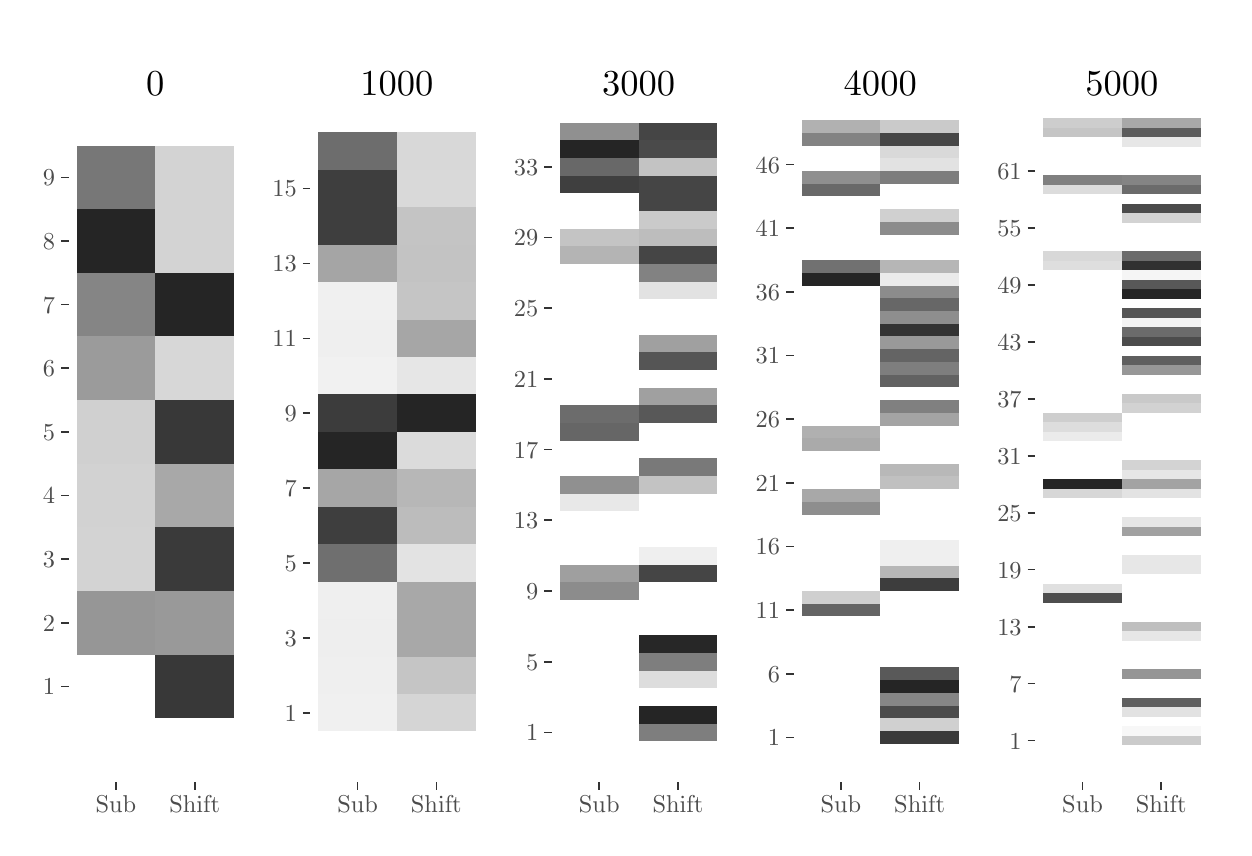
\begin{tikzpicture}[x=1pt,y=1pt]
\definecolor{fillColor}{RGB}{255,255,255}
\path[use as bounding box,fill=fillColor,fill opacity=0.00] (0,0) rectangle (432.17,289.08);
\begin{scope}
\path[clip] (  0.00,  0.00) rectangle ( 82.92,289.08);
\definecolor{drawColor}{RGB}{255,255,255}
\definecolor{fillColor}{RGB}{255,255,255}

\path[draw=drawColor,line width= 0.6pt,line join=round,line cap=round,fill=fillColor] (  0.00,  0.00) rectangle ( 82.92,289.08);
\end{scope}
\begin{scope}
\path[clip] ( 82.92,  0.00) rectangle (170.23,289.08);
\definecolor{drawColor}{RGB}{255,255,255}
\definecolor{fillColor}{RGB}{255,255,255}

\path[draw=drawColor,line width= 0.6pt,line join=round,line cap=round,fill=fillColor] ( 82.92,  0.00) rectangle (170.23,289.08);
\end{scope}
\begin{scope}
\path[clip] (170.23,  0.00) rectangle (257.55,289.08);
\definecolor{drawColor}{RGB}{255,255,255}
\definecolor{fillColor}{RGB}{255,255,255}

\path[draw=drawColor,line width= 0.6pt,line join=round,line cap=round,fill=fillColor] (170.23,  0.00) rectangle (257.55,289.08);
\end{scope}
\begin{scope}
\path[clip] (257.55,  0.00) rectangle (344.86,289.08);
\definecolor{drawColor}{RGB}{255,255,255}
\definecolor{fillColor}{RGB}{255,255,255}

\path[draw=drawColor,line width= 0.6pt,line join=round,line cap=round,fill=fillColor] (257.55,  0.00) rectangle (344.86,289.08);
\end{scope}
\begin{scope}
\path[clip] (344.86,  0.00) rectangle (432.17,289.08);
\definecolor{drawColor}{RGB}{255,255,255}
\definecolor{fillColor}{RGB}{255,255,255}

\path[draw=drawColor,line width= 0.6pt,line join=round,line cap=round,fill=fillColor] (344.86,  0.00) rectangle (432.17,289.08);
\end{scope}
\begin{scope}
\path[clip] ( 14.85, 16.51) rectangle ( 77.42,269.49);
\definecolor{drawColor}{RGB}{255,255,255}

\path[draw=drawColor,line width= 0.3pt,line join=round] ( 14.85, 28.01) --
	( 77.42, 28.01);

\path[draw=drawColor,line width= 0.3pt,line join=round] ( 14.85, 39.51) --
	( 77.42, 39.51);

\path[draw=drawColor,line width= 0.3pt,line join=round] ( 14.85, 62.51) --
	( 77.42, 62.51);

\path[draw=drawColor,line width= 0.3pt,line join=round] ( 14.85, 85.50) --
	( 77.42, 85.50);

\path[draw=drawColor,line width= 0.3pt,line join=round] ( 14.85,108.50) --
	( 77.42,108.50);

\path[draw=drawColor,line width= 0.3pt,line join=round] ( 14.85,131.50) --
	( 77.42,131.50);

\path[draw=drawColor,line width= 0.3pt,line join=round] ( 14.85,154.50) --
	( 77.42,154.50);

\path[draw=drawColor,line width= 0.3pt,line join=round] ( 14.85,177.50) --
	( 77.42,177.50);

\path[draw=drawColor,line width= 0.3pt,line join=round] ( 14.85,200.49) --
	( 77.42,200.49);

\path[draw=drawColor,line width= 0.3pt,line join=round] ( 14.85,223.49) --
	( 77.42,223.49);

\path[draw=drawColor,line width= 0.3pt,line join=round] ( 14.85,246.49) --
	( 77.42,246.49);

\path[draw=drawColor,line width= 0.3pt,line join=round] ( 14.85,257.99) --
	( 77.42,257.99);

\path[draw=drawColor,line width= 0.6pt,line join=round] ( 14.85, 51.01) --
	( 77.42, 51.01);

\path[draw=drawColor,line width= 0.6pt,line join=round] ( 14.85, 74.01) --
	( 77.42, 74.01);

\path[draw=drawColor,line width= 0.6pt,line join=round] ( 14.85, 97.00) --
	( 77.42, 97.00);

\path[draw=drawColor,line width= 0.6pt,line join=round] ( 14.85,120.00) --
	( 77.42,120.00);

\path[draw=drawColor,line width= 0.6pt,line join=round] ( 14.85,143.00) --
	( 77.42,143.00);

\path[draw=drawColor,line width= 0.6pt,line join=round] ( 14.85,166.00) --
	( 77.42,166.00);

\path[draw=drawColor,line width= 0.6pt,line join=round] ( 14.85,189.00) --
	( 77.42,189.00);

\path[draw=drawColor,line width= 0.6pt,line join=round] ( 14.85,211.99) --
	( 77.42,211.99);

\path[draw=drawColor,line width= 0.6pt,line join=round] ( 14.85,234.99) --
	( 77.42,234.99);

\path[draw=drawColor,line width= 0.6pt,line join=round] ( 31.91, 16.51) --
	( 31.91,269.49);

\path[draw=drawColor,line width= 0.6pt,line join=round] ( 60.35, 16.51) --
	( 60.35,269.49);
\definecolor{fillColor}{RGB}{255,255,255}

\path[fill=fillColor] ( 17.69, 39.51) rectangle ( 46.13, 62.51);
\definecolor{fillColor}{gray}{0.59}

\path[fill=fillColor] ( 17.69, 62.51) rectangle ( 46.13, 85.50);
\definecolor{fillColor}{RGB}{211,211,211}

\path[fill=fillColor] ( 17.69, 85.50) rectangle ( 46.13,108.50);
\definecolor{fillColor}{RGB}{210,210,210}

\path[fill=fillColor] ( 17.69,108.50) rectangle ( 46.13,131.50);
\definecolor{fillColor}{RGB}{208,208,208}

\path[fill=fillColor] ( 17.69,131.50) rectangle ( 46.13,154.50);
\definecolor{fillColor}{RGB}{155,155,155}

\path[fill=fillColor] ( 17.69,154.50) rectangle ( 46.13,177.50);
\definecolor{fillColor}{gray}{0.52}

\path[fill=fillColor] ( 17.69,177.50) rectangle ( 46.13,200.49);
\definecolor{fillColor}{RGB}{37,37,37}

\path[fill=fillColor] ( 17.69,200.49) rectangle ( 46.13,223.49);
\definecolor{fillColor}{RGB}{119,119,119}

\path[fill=fillColor] ( 17.69,223.49) rectangle ( 46.13,246.49);
\definecolor{fillColor}{gray}{0.22}

\path[fill=fillColor] ( 46.13, 39.51) rectangle ( 74.57, 62.51);
\definecolor{fillColor}{gray}{0.60}

\path[fill=fillColor] ( 46.13, 62.51) rectangle ( 74.57, 85.50);
\definecolor{fillColor}{RGB}{58,58,58}

\path[fill=fillColor] ( 46.13, 85.50) rectangle ( 74.57,108.50);
\definecolor{fillColor}{gray}{0.66}

\path[fill=fillColor] ( 46.13,108.50) rectangle ( 74.57,131.50);
\definecolor{fillColor}{gray}{0.22}

\path[fill=fillColor] ( 46.13,131.50) rectangle ( 74.57,154.50);
\definecolor{fillColor}{RGB}{215,215,215}

\path[fill=fillColor] ( 46.13,154.50) rectangle ( 74.57,177.50);
\definecolor{fillColor}{RGB}{37,37,37}

\path[fill=fillColor] ( 46.13,177.50) rectangle ( 74.57,200.49);
\definecolor{fillColor}{RGB}{211,211,211}

\path[fill=fillColor] ( 46.13,200.49) rectangle ( 74.57,223.49);

\path[fill=fillColor] ( 46.13,223.49) rectangle ( 74.57,246.49);
\end{scope}
\begin{scope}
\path[clip] (102.16, 16.51) rectangle (164.73,269.49);
\definecolor{drawColor}{RGB}{255,255,255}

\path[draw=drawColor,line width= 0.3pt,line join=round] (102.16, 28.01) --
	(164.73, 28.01);

\path[draw=drawColor,line width= 0.3pt,line join=round] (102.16, 55.07) --
	(164.73, 55.07);

\path[draw=drawColor,line width= 0.3pt,line join=round] (102.16, 82.12) --
	(164.73, 82.12);

\path[draw=drawColor,line width= 0.3pt,line join=round] (102.16,109.18) --
	(164.73,109.18);

\path[draw=drawColor,line width= 0.3pt,line join=round] (102.16,136.24) --
	(164.73,136.24);

\path[draw=drawColor,line width= 0.3pt,line join=round] (102.16,163.29) --
	(164.73,163.29);

\path[draw=drawColor,line width= 0.3pt,line join=round] (102.16,190.35) --
	(164.73,190.35);

\path[draw=drawColor,line width= 0.3pt,line join=round] (102.16,217.41) --
	(164.73,217.41);

\path[draw=drawColor,line width= 0.3pt,line join=round] (102.16,244.46) --
	(164.73,244.46);

\path[draw=drawColor,line width= 0.3pt,line join=round] (102.16,257.99) --
	(164.73,257.99);

\path[draw=drawColor,line width= 0.6pt,line join=round] (102.16, 41.54) --
	(164.73, 41.54);

\path[draw=drawColor,line width= 0.6pt,line join=round] (102.16, 68.59) --
	(164.73, 68.59);

\path[draw=drawColor,line width= 0.6pt,line join=round] (102.16, 95.65) --
	(164.73, 95.65);

\path[draw=drawColor,line width= 0.6pt,line join=round] (102.16,122.71) --
	(164.73,122.71);

\path[draw=drawColor,line width= 0.6pt,line join=round] (102.16,149.76) --
	(164.73,149.76);

\path[draw=drawColor,line width= 0.6pt,line join=round] (102.16,176.82) --
	(164.73,176.82);

\path[draw=drawColor,line width= 0.6pt,line join=round] (102.16,203.88) --
	(164.73,203.88);

\path[draw=drawColor,line width= 0.6pt,line join=round] (102.16,230.93) --
	(164.73,230.93);

\path[draw=drawColor,line width= 0.6pt,line join=round] (119.23, 16.51) --
	(119.23,269.49);

\path[draw=drawColor,line width= 0.6pt,line join=round] (147.67, 16.51) --
	(147.67,269.49);
\definecolor{fillColor}{gray}{0.94}

\path[fill=fillColor] (105.01, 34.77) rectangle (133.45, 48.30);
\definecolor{fillColor}{RGB}{239,239,239}

\path[fill=fillColor] (105.01, 48.30) rectangle (133.45, 61.83);
\definecolor{fillColor}{RGB}{238,238,238}

\path[fill=fillColor] (105.01, 61.83) rectangle (133.45, 75.36);
\definecolor{fillColor}{RGB}{239,239,239}

\path[fill=fillColor] (105.01, 75.36) rectangle (133.45, 88.89);
\definecolor{fillColor}{RGB}{111,111,111}

\path[fill=fillColor] (105.01, 88.89) rectangle (133.45,102.42);
\definecolor{fillColor}{RGB}{62,62,62}

\path[fill=fillColor] (105.01,102.42) rectangle (133.45,115.94);
\definecolor{fillColor}{gray}{0.65}

\path[fill=fillColor] (105.01,115.94) rectangle (133.45,129.47);
\definecolor{fillColor}{RGB}{37,37,37}

\path[fill=fillColor] (105.01,129.47) rectangle (133.45,143.00);
\definecolor{fillColor}{RGB}{60,60,60}

\path[fill=fillColor] (105.01,143.00) rectangle (133.45,156.53);
\definecolor{fillColor}{RGB}{241,241,241}

\path[fill=fillColor] (105.01,156.53) rectangle (133.45,170.06);
\definecolor{fillColor}{RGB}{239,239,239}

\path[fill=fillColor] (105.01,170.06) rectangle (133.45,183.58);
\definecolor{fillColor}{gray}{0.94}

\path[fill=fillColor] (105.01,183.58) rectangle (133.45,197.11);
\definecolor{fillColor}{RGB}{165,165,165}

\path[fill=fillColor] (105.01,197.11) rectangle (133.45,210.64);
\definecolor{fillColor}{RGB}{62,62,62}

\path[fill=fillColor] (105.01,210.64) rectangle (133.45,224.17);

\path[fill=fillColor] (105.01,224.17) rectangle (133.45,237.70);
\definecolor{fillColor}{RGB}{109,109,109}

\path[fill=fillColor] (105.01,237.70) rectangle (133.45,251.23);
\definecolor{fillColor}{RGB}{213,213,213}

\path[fill=fillColor] (133.45, 34.77) rectangle (161.89, 48.30);
\definecolor{fillColor}{RGB}{197,197,197}

\path[fill=fillColor] (133.45, 48.30) rectangle (161.89, 61.83);
\definecolor{fillColor}{gray}{0.66}

\path[fill=fillColor] (133.45, 61.83) rectangle (161.89, 75.36);

\path[fill=fillColor] (133.45, 75.36) rectangle (161.89, 88.89);
\definecolor{fillColor}{gray}{0.89}

\path[fill=fillColor] (133.45, 88.89) rectangle (161.89,102.42);
\definecolor{fillColor}{RGB}{188,188,188}

\path[fill=fillColor] (133.45,102.42) rectangle (161.89,115.94);
\definecolor{fillColor}{RGB}{183,183,183}

\path[fill=fillColor] (133.45,115.94) rectangle (161.89,129.47);
\definecolor{fillColor}{gray}{0.86}

\path[fill=fillColor] (133.45,129.47) rectangle (161.89,143.00);
\definecolor{fillColor}{RGB}{37,37,37}

\path[fill=fillColor] (133.45,143.00) rectangle (161.89,156.53);
\definecolor{fillColor}{RGB}{230,230,230}

\path[fill=fillColor] (133.45,156.53) rectangle (161.89,170.06);
\definecolor{fillColor}{gray}{0.65}

\path[fill=fillColor] (133.45,170.06) rectangle (161.89,183.58);
\definecolor{fillColor}{RGB}{197,197,197}

\path[fill=fillColor] (133.45,183.58) rectangle (161.89,197.11);
\definecolor{fillColor}{RGB}{195,195,195}

\path[fill=fillColor] (133.45,197.11) rectangle (161.89,210.64);
\definecolor{fillColor}{gray}{0.77}

\path[fill=fillColor] (133.45,210.64) rectangle (161.89,224.17);
\definecolor{fillColor}{gray}{0.85}

\path[fill=fillColor] (133.45,224.17) rectangle (161.89,237.70);
\definecolor{fillColor}{RGB}{216,216,216}

\path[fill=fillColor] (133.45,237.70) rectangle (161.89,251.23);
\end{scope}
\begin{scope}
\path[clip] (189.48, 16.51) rectangle (252.05,269.49);
\definecolor{drawColor}{RGB}{255,255,255}

\path[draw=drawColor,line width= 0.3pt,line join=round] (189.48, 21.62) --
	(252.05, 21.62);

\path[draw=drawColor,line width= 0.3pt,line join=round] (189.48, 47.17) --
	(252.05, 47.17);

\path[draw=drawColor,line width= 0.3pt,line join=round] (189.48, 72.73) --
	(252.05, 72.73);

\path[draw=drawColor,line width= 0.3pt,line join=round] (189.48, 98.28) --
	(252.05, 98.28);

\path[draw=drawColor,line width= 0.3pt,line join=round] (189.48,123.83) --
	(252.05,123.83);

\path[draw=drawColor,line width= 0.3pt,line join=round] (189.48,149.39) --
	(252.05,149.39);

\path[draw=drawColor,line width= 0.3pt,line join=round] (189.48,174.94) --
	(252.05,174.94);

\path[draw=drawColor,line width= 0.3pt,line join=round] (189.48,200.49) --
	(252.05,200.49);

\path[draw=drawColor,line width= 0.3pt,line join=round] (189.48,226.05) --
	(252.05,226.05);

\path[draw=drawColor,line width= 0.3pt,line join=round] (189.48,251.60) --
	(252.05,251.60);

\path[draw=drawColor,line width= 0.3pt,line join=round] (189.48,264.38) --
	(252.05,264.38);

\path[draw=drawColor,line width= 0.6pt,line join=round] (189.48, 34.40) --
	(252.05, 34.40);

\path[draw=drawColor,line width= 0.6pt,line join=round] (189.48, 59.95) --
	(252.05, 59.95);

\path[draw=drawColor,line width= 0.6pt,line join=round] (189.48, 85.50) --
	(252.05, 85.50);

\path[draw=drawColor,line width= 0.6pt,line join=round] (189.48,111.06) --
	(252.05,111.06);

\path[draw=drawColor,line width= 0.6pt,line join=round] (189.48,136.61) --
	(252.05,136.61);

\path[draw=drawColor,line width= 0.6pt,line join=round] (189.48,162.16) --
	(252.05,162.16);

\path[draw=drawColor,line width= 0.6pt,line join=round] (189.48,187.72) --
	(252.05,187.72);

\path[draw=drawColor,line width= 0.6pt,line join=round] (189.48,213.27) --
	(252.05,213.27);

\path[draw=drawColor,line width= 0.6pt,line join=round] (189.48,238.82) --
	(252.05,238.82);

\path[draw=drawColor,line width= 0.6pt,line join=round] (206.54, 16.51) --
	(206.54,269.49);

\path[draw=drawColor,line width= 0.6pt,line join=round] (234.98, 16.51) --
	(234.98,269.49);
\definecolor{fillColor}{RGB}{255,255,255}

\path[fill=fillColor] (192.32, 31.20) rectangle (220.76, 37.59);

\path[fill=fillColor] (192.32, 37.59) rectangle (220.76, 43.98);

\path[fill=fillColor] (192.32, 43.98) rectangle (220.76, 50.37);

\path[fill=fillColor] (192.32, 50.37) rectangle (220.76, 56.76);

\path[fill=fillColor] (192.32, 56.76) rectangle (220.76, 63.15);

\path[fill=fillColor] (192.32, 63.15) rectangle (220.76, 69.53);

\path[fill=fillColor] (192.32, 69.53) rectangle (220.76, 75.92);

\path[fill=fillColor] (192.32, 75.92) rectangle (220.76, 82.31);
\definecolor{fillColor}{gray}{0.55}

\path[fill=fillColor] (192.32, 82.31) rectangle (220.76, 88.70);
\definecolor{fillColor}{RGB}{159,159,159}

\path[fill=fillColor] (192.32, 88.70) rectangle (220.76, 95.09);
\definecolor{fillColor}{RGB}{255,255,255}

\path[fill=fillColor] (192.32, 95.09) rectangle (220.76,101.48);

\path[fill=fillColor] (192.32,101.48) rectangle (220.76,107.86);

\path[fill=fillColor] (192.32,107.86) rectangle (220.76,114.25);
\definecolor{fillColor}{gray}{0.91}

\path[fill=fillColor] (192.32,114.25) rectangle (220.76,120.64);
\definecolor{fillColor}{RGB}{144,144,144}

\path[fill=fillColor] (192.32,120.64) rectangle (220.76,127.03);
\definecolor{fillColor}{RGB}{255,255,255}

\path[fill=fillColor] (192.32,127.03) rectangle (220.76,133.42);

\path[fill=fillColor] (192.32,133.42) rectangle (220.76,139.81);
\definecolor{fillColor}{gray}{0.40}

\path[fill=fillColor] (192.32,139.81) rectangle (220.76,146.19);
\definecolor{fillColor}{RGB}{108,108,108}

\path[fill=fillColor] (192.32,146.19) rectangle (220.76,152.58);
\definecolor{fillColor}{RGB}{255,255,255}

\path[fill=fillColor] (192.32,152.58) rectangle (220.76,158.97);

\path[fill=fillColor] (192.32,158.97) rectangle (220.76,165.36);

\path[fill=fillColor] (192.32,165.36) rectangle (220.76,171.75);

\path[fill=fillColor] (192.32,171.75) rectangle (220.76,178.14);

\path[fill=fillColor] (192.32,178.14) rectangle (220.76,184.52);

\path[fill=fillColor] (192.32,184.52) rectangle (220.76,190.91);

\path[fill=fillColor] (192.32,190.91) rectangle (220.76,197.30);

\path[fill=fillColor] (192.32,197.30) rectangle (220.76,203.69);
\definecolor{fillColor}{RGB}{180,180,180}

\path[fill=fillColor] (192.32,203.69) rectangle (220.76,210.08);
\definecolor{fillColor}{gray}{0.77}

\path[fill=fillColor] (192.32,210.08) rectangle (220.76,216.47);
\definecolor{fillColor}{RGB}{255,255,255}

\path[fill=fillColor] (192.32,216.47) rectangle (220.76,222.85);

\path[fill=fillColor] (192.32,222.85) rectangle (220.76,229.24);
\definecolor{fillColor}{RGB}{63,63,63}

\path[fill=fillColor] (192.32,229.24) rectangle (220.76,235.63);
\definecolor{fillColor}{RGB}{104,104,104}

\path[fill=fillColor] (192.32,235.63) rectangle (220.76,242.02);
\definecolor{fillColor}{RGB}{37,37,37}

\path[fill=fillColor] (192.32,242.02) rectangle (220.76,248.41);
\definecolor{fillColor}{RGB}{144,144,144}

\path[fill=fillColor] (192.32,248.41) rectangle (220.76,254.80);
\definecolor{fillColor}{RGB}{126,126,126}

\path[fill=fillColor] (220.76, 31.20) rectangle (249.20, 37.59);
\definecolor{fillColor}{RGB}{37,37,37}

\path[fill=fillColor] (220.76, 37.59) rectangle (249.20, 43.98);
\definecolor{fillColor}{RGB}{255,255,255}

\path[fill=fillColor] (220.76, 43.98) rectangle (249.20, 50.37);
\definecolor{fillColor}{RGB}{221,221,221}

\path[fill=fillColor] (220.76, 50.37) rectangle (249.20, 56.76);
\definecolor{fillColor}{RGB}{126,126,126}

\path[fill=fillColor] (220.76, 56.76) rectangle (249.20, 63.15);
\definecolor{fillColor}{RGB}{39,39,39}

\path[fill=fillColor] (220.76, 63.15) rectangle (249.20, 69.53);
\definecolor{fillColor}{RGB}{255,255,255}

\path[fill=fillColor] (220.76, 69.53) rectangle (249.20, 75.92);

\path[fill=fillColor] (220.76, 75.92) rectangle (249.20, 82.31);

\path[fill=fillColor] (220.76, 82.31) rectangle (249.20, 88.70);
\definecolor{fillColor}{gray}{0.27}

\path[fill=fillColor] (220.76, 88.70) rectangle (249.20, 95.09);
\definecolor{fillColor}{RGB}{239,239,239}

\path[fill=fillColor] (220.76, 95.09) rectangle (249.20,101.48);
\definecolor{fillColor}{RGB}{255,255,255}

\path[fill=fillColor] (220.76,101.48) rectangle (249.20,107.86);

\path[fill=fillColor] (220.76,107.86) rectangle (249.20,114.25);

\path[fill=fillColor] (220.76,114.25) rectangle (249.20,120.64);
\definecolor{fillColor}{RGB}{195,195,195}

\path[fill=fillColor] (220.76,120.64) rectangle (249.20,127.03);
\definecolor{fillColor}{RGB}{121,121,121}

\path[fill=fillColor] (220.76,127.03) rectangle (249.20,133.42);
\definecolor{fillColor}{RGB}{255,255,255}

\path[fill=fillColor] (220.76,133.42) rectangle (249.20,139.81);

\path[fill=fillColor] (220.76,139.81) rectangle (249.20,146.19);
\definecolor{fillColor}{RGB}{88,88,88}

\path[fill=fillColor] (220.76,146.19) rectangle (249.20,152.58);
\definecolor{fillColor}{RGB}{160,160,160}

\path[fill=fillColor] (220.76,152.58) rectangle (249.20,158.97);
\definecolor{fillColor}{RGB}{255,255,255}

\path[fill=fillColor] (220.76,158.97) rectangle (249.20,165.36);
\definecolor{fillColor}{RGB}{85,85,85}

\path[fill=fillColor] (220.76,165.36) rectangle (249.20,171.75);
\definecolor{fillColor}{RGB}{160,160,160}

\path[fill=fillColor] (220.76,171.75) rectangle (249.20,178.14);
\definecolor{fillColor}{RGB}{255,255,255}

\path[fill=fillColor] (220.76,178.14) rectangle (249.20,184.52);

\path[fill=fillColor] (220.76,184.52) rectangle (249.20,190.91);
\definecolor{fillColor}{RGB}{226,226,226}

\path[fill=fillColor] (220.76,190.91) rectangle (249.20,197.30);
\definecolor{fillColor}{gray}{0.51}

\path[fill=fillColor] (220.76,197.30) rectangle (249.20,203.69);
\definecolor{fillColor}{gray}{0.27}

\path[fill=fillColor] (220.76,203.69) rectangle (249.20,210.08);
\definecolor{fillColor}{gray}{0.74}

\path[fill=fillColor] (220.76,210.08) rectangle (249.20,216.47);
\definecolor{fillColor}{RGB}{202,202,202}

\path[fill=fillColor] (220.76,216.47) rectangle (249.20,222.85);
\definecolor{fillColor}{gray}{0.27}

\path[fill=fillColor] (220.76,222.85) rectangle (249.20,229.24);

\path[fill=fillColor] (220.76,229.24) rectangle (249.20,235.63);
\definecolor{fillColor}{RGB}{195,195,195}

\path[fill=fillColor] (220.76,235.63) rectangle (249.20,242.02);
\definecolor{fillColor}{gray}{0.29}

\path[fill=fillColor] (220.76,242.02) rectangle (249.20,248.41);
\definecolor{fillColor}{gray}{0.27}

\path[fill=fillColor] (220.76,248.41) rectangle (249.20,254.80);
\end{scope}
\begin{scope}
\path[clip] (276.79, 16.51) rectangle (339.36,269.49);
\definecolor{drawColor}{RGB}{255,255,255}

\path[draw=drawColor,line width= 0.3pt,line join=round] (276.79, 21.11) --
	(339.36, 21.11);

\path[draw=drawColor,line width= 0.3pt,line join=round] (276.79, 44.11) --
	(339.36, 44.11);

\path[draw=drawColor,line width= 0.3pt,line join=round] (276.79, 67.11) --
	(339.36, 67.11);

\path[draw=drawColor,line width= 0.3pt,line join=round] (276.79, 90.10) --
	(339.36, 90.10);

\path[draw=drawColor,line width= 0.3pt,line join=round] (276.79,113.10) --
	(339.36,113.10);

\path[draw=drawColor,line width= 0.3pt,line join=round] (276.79,136.10) --
	(339.36,136.10);

\path[draw=drawColor,line width= 0.3pt,line join=round] (276.79,159.10) --
	(339.36,159.10);

\path[draw=drawColor,line width= 0.3pt,line join=round] (276.79,182.10) --
	(339.36,182.10);

\path[draw=drawColor,line width= 0.3pt,line join=round] (276.79,205.09) --
	(339.36,205.09);

\path[draw=drawColor,line width= 0.3pt,line join=round] (276.79,228.09) --
	(339.36,228.09);

\path[draw=drawColor,line width= 0.3pt,line join=round] (276.79,251.09) --
	(339.36,251.09);

\path[draw=drawColor,line width= 0.3pt,line join=round] (276.79,262.59) --
	(339.36,262.59);

\path[draw=drawColor,line width= 0.6pt,line join=round] (276.79, 32.61) --
	(339.36, 32.61);

\path[draw=drawColor,line width= 0.6pt,line join=round] (276.79, 55.61) --
	(339.36, 55.61);

\path[draw=drawColor,line width= 0.6pt,line join=round] (276.79, 78.61) --
	(339.36, 78.61);

\path[draw=drawColor,line width= 0.6pt,line join=round] (276.79,101.60) --
	(339.36,101.60);

\path[draw=drawColor,line width= 0.6pt,line join=round] (276.79,124.60) --
	(339.36,124.60);

\path[draw=drawColor,line width= 0.6pt,line join=round] (276.79,147.60) --
	(339.36,147.60);

\path[draw=drawColor,line width= 0.6pt,line join=round] (276.79,170.60) --
	(339.36,170.60);

\path[draw=drawColor,line width= 0.6pt,line join=round] (276.79,193.60) --
	(339.36,193.60);

\path[draw=drawColor,line width= 0.6pt,line join=round] (276.79,216.59) --
	(339.36,216.59);

\path[draw=drawColor,line width= 0.6pt,line join=round] (276.79,239.59) --
	(339.36,239.59);

\path[draw=drawColor,line width= 0.6pt,line join=round] (293.86, 16.51) --
	(293.86,269.49);

\path[draw=drawColor,line width= 0.6pt,line join=round] (322.30, 16.51) --
	(322.30,269.49);
\definecolor{fillColor}{RGB}{255,255,255}

\path[fill=fillColor] (279.64, 30.31) rectangle (308.08, 34.91);

\path[fill=fillColor] (279.64, 34.91) rectangle (308.08, 39.51);

\path[fill=fillColor] (279.64, 39.51) rectangle (308.08, 44.11);

\path[fill=fillColor] (279.64, 44.11) rectangle (308.08, 48.71);

\path[fill=fillColor] (279.64, 48.71) rectangle (308.08, 53.31);

\path[fill=fillColor] (279.64, 53.31) rectangle (308.08, 57.91);

\path[fill=fillColor] (279.64, 57.91) rectangle (308.08, 62.51);

\path[fill=fillColor] (279.64, 62.51) rectangle (308.08, 67.11);

\path[fill=fillColor] (279.64, 67.11) rectangle (308.08, 71.71);

\path[fill=fillColor] (279.64, 71.71) rectangle (308.08, 76.31);
\definecolor{fillColor}{RGB}{100,100,100}

\path[fill=fillColor] (279.64, 76.31) rectangle (308.08, 80.91);
\definecolor{fillColor}{gray}{0.81}

\path[fill=fillColor] (279.64, 80.91) rectangle (308.08, 85.50);
\definecolor{fillColor}{RGB}{255,255,255}

\path[fill=fillColor] (279.64, 85.50) rectangle (308.08, 90.10);

\path[fill=fillColor] (279.64, 90.10) rectangle (308.08, 94.70);

\path[fill=fillColor] (279.64, 94.70) rectangle (308.08, 99.30);

\path[fill=fillColor] (279.64, 99.30) rectangle (308.08,103.90);

\path[fill=fillColor] (279.64,103.90) rectangle (308.08,108.50);

\path[fill=fillColor] (279.64,108.50) rectangle (308.08,113.10);
\definecolor{fillColor}{RGB}{142,142,142}

\path[fill=fillColor] (279.64,113.10) rectangle (308.08,117.70);
\definecolor{fillColor}{gray}{0.66}

\path[fill=fillColor] (279.64,117.70) rectangle (308.08,122.30);
\definecolor{fillColor}{RGB}{255,255,255}

\path[fill=fillColor] (279.64,122.30) rectangle (308.08,126.90);

\path[fill=fillColor] (279.64,126.90) rectangle (308.08,131.50);

\path[fill=fillColor] (279.64,131.50) rectangle (308.08,136.10);
\definecolor{fillColor}{RGB}{170,170,170}

\path[fill=fillColor] (279.64,136.10) rectangle (308.08,140.70);
\definecolor{fillColor}{gray}{0.69}

\path[fill=fillColor] (279.64,140.70) rectangle (308.08,145.30);
\definecolor{fillColor}{RGB}{255,255,255}

\path[fill=fillColor] (279.64,145.30) rectangle (308.08,149.90);

\path[fill=fillColor] (279.64,149.90) rectangle (308.08,154.50);

\path[fill=fillColor] (279.64,154.50) rectangle (308.08,159.10);

\path[fill=fillColor] (279.64,159.10) rectangle (308.08,163.70);

\path[fill=fillColor] (279.64,163.70) rectangle (308.08,168.30);

\path[fill=fillColor] (279.64,168.30) rectangle (308.08,172.90);

\path[fill=fillColor] (279.64,172.90) rectangle (308.08,177.50);

\path[fill=fillColor] (279.64,177.50) rectangle (308.08,182.10);

\path[fill=fillColor] (279.64,182.10) rectangle (308.08,186.70);

\path[fill=fillColor] (279.64,186.70) rectangle (308.08,191.30);

\path[fill=fillColor] (279.64,191.30) rectangle (308.08,195.90);
\definecolor{fillColor}{RGB}{37,37,37}

\path[fill=fillColor] (279.64,195.90) rectangle (308.08,200.49);
\definecolor{fillColor}{RGB}{113,113,113}

\path[fill=fillColor] (279.64,200.49) rectangle (308.08,205.09);
\definecolor{fillColor}{RGB}{255,255,255}

\path[fill=fillColor] (279.64,205.09) rectangle (308.08,209.69);

\path[fill=fillColor] (279.64,209.69) rectangle (308.08,214.29);

\path[fill=fillColor] (279.64,214.29) rectangle (308.08,218.89);

\path[fill=fillColor] (279.64,218.89) rectangle (308.08,223.49);

\path[fill=fillColor] (279.64,223.49) rectangle (308.08,228.09);
\definecolor{fillColor}{RGB}{105,105,105}

\path[fill=fillColor] (279.64,228.09) rectangle (308.08,232.69);
\definecolor{fillColor}{gray}{0.56}

\path[fill=fillColor] (279.64,232.69) rectangle (308.08,237.29);
\definecolor{fillColor}{RGB}{255,255,255}

\path[fill=fillColor] (279.64,237.29) rectangle (308.08,241.89);

\path[fill=fillColor] (279.64,241.89) rectangle (308.08,246.49);
\definecolor{fillColor}{RGB}{131,131,131}

\path[fill=fillColor] (279.64,246.49) rectangle (308.08,251.09);
\definecolor{fillColor}{RGB}{177,177,177}

\path[fill=fillColor] (279.64,251.09) rectangle (308.08,255.69);
\definecolor{fillColor}{RGB}{58,58,58}

\path[fill=fillColor] (308.08, 30.31) rectangle (336.52, 34.91);
\definecolor{fillColor}{RGB}{208,208,208}

\path[fill=fillColor] (308.08, 34.91) rectangle (336.52, 39.51);
\definecolor{fillColor}{RGB}{75,75,75}

\path[fill=fillColor] (308.08, 39.51) rectangle (336.52, 44.11);
\definecolor{fillColor}{RGB}{134,134,134}

\path[fill=fillColor] (308.08, 44.11) rectangle (336.52, 48.71);
\definecolor{fillColor}{RGB}{37,37,37}

\path[fill=fillColor] (308.08, 48.71) rectangle (336.52, 53.31);
\definecolor{fillColor}{gray}{0.35}

\path[fill=fillColor] (308.08, 53.31) rectangle (336.52, 57.91);
\definecolor{fillColor}{RGB}{255,255,255}

\path[fill=fillColor] (308.08, 57.91) rectangle (336.52, 62.51);

\path[fill=fillColor] (308.08, 62.51) rectangle (336.52, 67.11);

\path[fill=fillColor] (308.08, 67.11) rectangle (336.52, 71.71);

\path[fill=fillColor] (308.08, 71.71) rectangle (336.52, 76.31);

\path[fill=fillColor] (308.08, 76.31) rectangle (336.52, 80.91);

\path[fill=fillColor] (308.08, 80.91) rectangle (336.52, 85.50);
\definecolor{fillColor}{gray}{0.24}

\path[fill=fillColor] (308.08, 85.50) rectangle (336.52, 90.10);
\definecolor{fillColor}{RGB}{183,183,183}

\path[fill=fillColor] (308.08, 90.10) rectangle (336.52, 94.70);
\definecolor{fillColor}{RGB}{239,239,239}

\path[fill=fillColor] (308.08, 94.70) rectangle (336.52, 99.30);

\path[fill=fillColor] (308.08, 99.30) rectangle (336.52,103.90);
\definecolor{fillColor}{RGB}{255,255,255}

\path[fill=fillColor] (308.08,103.90) rectangle (336.52,108.50);

\path[fill=fillColor] (308.08,108.50) rectangle (336.52,113.10);

\path[fill=fillColor] (308.08,113.10) rectangle (336.52,117.70);

\path[fill=fillColor] (308.08,117.70) rectangle (336.52,122.30);
\definecolor{fillColor}{RGB}{192,192,192}

\path[fill=fillColor] (308.08,122.30) rectangle (336.52,126.90);
\definecolor{fillColor}{gray}{0.72}

\path[fill=fillColor] (308.08,126.90) rectangle (336.52,131.50);
\definecolor{fillColor}{RGB}{255,255,255}

\path[fill=fillColor] (308.08,131.50) rectangle (336.52,136.10);

\path[fill=fillColor] (308.08,136.10) rectangle (336.52,140.70);

\path[fill=fillColor] (308.08,140.70) rectangle (336.52,145.30);
\definecolor{fillColor}{RGB}{164,164,164}

\path[fill=fillColor] (308.08,145.30) rectangle (336.52,149.90);
\definecolor{fillColor}{gray}{0.50}

\path[fill=fillColor] (308.08,149.90) rectangle (336.52,154.50);
\definecolor{fillColor}{RGB}{255,255,255}

\path[fill=fillColor] (308.08,154.50) rectangle (336.52,159.10);
\definecolor{fillColor}{RGB}{98,98,98}

\path[fill=fillColor] (308.08,159.10) rectangle (336.52,163.70);
\definecolor{fillColor}{RGB}{126,126,126}

\path[fill=fillColor] (308.08,163.70) rectangle (336.52,168.30);
\definecolor{fillColor}{RGB}{100,100,100}

\path[fill=fillColor] (308.08,168.30) rectangle (336.52,172.90);
\definecolor{fillColor}{gray}{0.60}

\path[fill=fillColor] (308.08,172.90) rectangle (336.52,177.50);
\definecolor{fillColor}{gray}{0.20}

\path[fill=fillColor] (308.08,177.50) rectangle (336.52,182.10);
\definecolor{fillColor}{RGB}{142,142,142}

\path[fill=fillColor] (308.08,182.10) rectangle (336.52,186.70);
\definecolor{fillColor}{RGB}{103,103,103}

\path[fill=fillColor] (308.08,186.70) rectangle (336.52,191.30);
\definecolor{fillColor}{gray}{0.55}

\path[fill=fillColor] (308.08,191.30) rectangle (336.52,195.90);
\definecolor{fillColor}{gray}{0.92}

\path[fill=fillColor] (308.08,195.90) rectangle (336.52,200.49);
\definecolor{fillColor}{RGB}{182,182,182}

\path[fill=fillColor] (308.08,200.49) rectangle (336.52,205.09);
\definecolor{fillColor}{RGB}{255,255,255}

\path[fill=fillColor] (308.08,205.09) rectangle (336.52,209.69);

\path[fill=fillColor] (308.08,209.69) rectangle (336.52,214.29);
\definecolor{fillColor}{gray}{0.55}

\path[fill=fillColor] (308.08,214.29) rectangle (336.52,218.89);
\definecolor{fillColor}{RGB}{208,208,208}

\path[fill=fillColor] (308.08,218.89) rectangle (336.52,223.49);
\definecolor{fillColor}{RGB}{255,255,255}

\path[fill=fillColor] (308.08,223.49) rectangle (336.52,228.09);

\path[fill=fillColor] (308.08,228.09) rectangle (336.52,232.69);
\definecolor{fillColor}{gray}{0.49}

\path[fill=fillColor] (308.08,232.69) rectangle (336.52,237.29);
\definecolor{fillColor}{RGB}{226,226,226}

\path[fill=fillColor] (308.08,237.29) rectangle (336.52,241.89);
\definecolor{fillColor}{gray}{0.85}

\path[fill=fillColor] (308.08,241.89) rectangle (336.52,246.49);
\definecolor{fillColor}{RGB}{70,70,70}

\path[fill=fillColor] (308.08,246.49) rectangle (336.52,251.09);
\definecolor{fillColor}{RGB}{202,202,202}

\path[fill=fillColor] (308.08,251.09) rectangle (336.52,255.69);
\end{scope}
\begin{scope}
\path[clip] (364.11, 16.51) rectangle (426.67,269.49);
\definecolor{drawColor}{RGB}{255,255,255}

\path[draw=drawColor,line width= 0.3pt,line join=round] (364.11, 21.14) --
	(426.67, 21.14);

\path[draw=drawColor,line width= 0.3pt,line join=round] (364.11, 41.74) --
	(426.67, 41.74);

\path[draw=drawColor,line width= 0.3pt,line join=round] (364.11, 62.34) --
	(426.67, 62.34);

\path[draw=drawColor,line width= 0.3pt,line join=round] (364.11, 82.93) --
	(426.67, 82.93);

\path[draw=drawColor,line width= 0.3pt,line join=round] (364.11,103.53) --
	(426.67,103.53);

\path[draw=drawColor,line width= 0.3pt,line join=round] (364.11,124.12) --
	(426.67,124.12);

\path[draw=drawColor,line width= 0.3pt,line join=round] (364.11,144.72) --
	(426.67,144.72);

\path[draw=drawColor,line width= 0.3pt,line join=round] (364.11,165.31) --
	(426.67,165.31);

\path[draw=drawColor,line width= 0.3pt,line join=round] (364.11,185.91) --
	(426.67,185.91);

\path[draw=drawColor,line width= 0.3pt,line join=round] (364.11,206.50) --
	(426.67,206.50);

\path[draw=drawColor,line width= 0.3pt,line join=round] (364.11,227.10) --
	(426.67,227.10);

\path[draw=drawColor,line width= 0.3pt,line join=round] (364.11,247.69) --
	(426.67,247.69);

\path[draw=drawColor,line width= 0.3pt,line join=round] (364.11,257.99) --
	(426.67,257.99);

\path[draw=drawColor,line width= 0.6pt,line join=round] (364.11, 31.44) --
	(426.67, 31.44);

\path[draw=drawColor,line width= 0.6pt,line join=round] (364.11, 52.04) --
	(426.67, 52.04);

\path[draw=drawColor,line width= 0.6pt,line join=round] (364.11, 72.63) --
	(426.67, 72.63);

\path[draw=drawColor,line width= 0.6pt,line join=round] (364.11, 93.23) --
	(426.67, 93.23);

\path[draw=drawColor,line width= 0.6pt,line join=round] (364.11,113.82) --
	(426.67,113.82);

\path[draw=drawColor,line width= 0.6pt,line join=round] (364.11,134.42) --
	(426.67,134.42);

\path[draw=drawColor,line width= 0.6pt,line join=round] (364.11,155.01) --
	(426.67,155.01);

\path[draw=drawColor,line width= 0.6pt,line join=round] (364.11,175.61) --
	(426.67,175.61);

\path[draw=drawColor,line width= 0.6pt,line join=round] (364.11,196.20) --
	(426.67,196.20);

\path[draw=drawColor,line width= 0.6pt,line join=round] (364.11,216.80) --
	(426.67,216.80);

\path[draw=drawColor,line width= 0.6pt,line join=round] (364.11,237.39) --
	(426.67,237.39);

\path[draw=drawColor,line width= 0.6pt,line join=round] (381.17, 16.51) --
	(381.17,269.49);

\path[draw=drawColor,line width= 0.6pt,line join=round] (409.61, 16.51) --
	(409.61,269.49);
\definecolor{fillColor}{RGB}{255,255,255}

\path[fill=fillColor] (366.95, 29.73) rectangle (395.39, 33.16);

\path[fill=fillColor] (366.95, 33.16) rectangle (395.39, 36.59);

\path[fill=fillColor] (366.95, 36.59) rectangle (395.39, 40.02);

\path[fill=fillColor] (366.95, 40.02) rectangle (395.39, 43.46);

\path[fill=fillColor] (366.95, 43.46) rectangle (395.39, 46.89);

\path[fill=fillColor] (366.95, 46.89) rectangle (395.39, 50.32);

\path[fill=fillColor] (366.95, 50.32) rectangle (395.39, 53.75);

\path[fill=fillColor] (366.95, 53.75) rectangle (395.39, 57.19);

\path[fill=fillColor] (366.95, 57.19) rectangle (395.39, 60.62);

\path[fill=fillColor] (366.95, 60.62) rectangle (395.39, 64.05);

\path[fill=fillColor] (366.95, 64.05) rectangle (395.39, 67.48);

\path[fill=fillColor] (366.95, 67.48) rectangle (395.39, 70.92);

\path[fill=fillColor] (366.95, 70.92) rectangle (395.39, 74.35);

\path[fill=fillColor] (366.95, 74.35) rectangle (395.39, 77.78);

\path[fill=fillColor] (366.95, 77.78) rectangle (395.39, 81.21);
\definecolor{fillColor}{RGB}{78,78,78}

\path[fill=fillColor] (366.95, 81.21) rectangle (395.39, 84.65);
\definecolor{fillColor}{gray}{0.88}

\path[fill=fillColor] (366.95, 84.65) rectangle (395.39, 88.08);
\definecolor{fillColor}{RGB}{255,255,255}

\path[fill=fillColor] (366.95, 88.08) rectangle (395.39, 91.51);

\path[fill=fillColor] (366.95, 91.51) rectangle (395.39, 94.94);

\path[fill=fillColor] (366.95, 94.94) rectangle (395.39, 98.38);

\path[fill=fillColor] (366.95, 98.38) rectangle (395.39,101.81);

\path[fill=fillColor] (366.95,101.81) rectangle (395.39,105.24);

\path[fill=fillColor] (366.95,105.24) rectangle (395.39,108.67);

\path[fill=fillColor] (366.95,108.67) rectangle (395.39,112.11);

\path[fill=fillColor] (366.95,112.11) rectangle (395.39,115.54);

\path[fill=fillColor] (366.95,115.54) rectangle (395.39,118.97);
\definecolor{fillColor}{RGB}{215,215,215}

\path[fill=fillColor] (366.95,118.97) rectangle (395.39,122.40);
\definecolor{fillColor}{RGB}{37,37,37}

\path[fill=fillColor] (366.95,122.40) rectangle (395.39,125.84);
\definecolor{fillColor}{RGB}{255,255,255}

\path[fill=fillColor] (366.95,125.84) rectangle (395.39,129.27);

\path[fill=fillColor] (366.95,129.27) rectangle (395.39,132.70);

\path[fill=fillColor] (366.95,132.70) rectangle (395.39,136.13);

\path[fill=fillColor] (366.95,136.13) rectangle (395.39,139.57);
\definecolor{fillColor}{gray}{0.92}

\path[fill=fillColor] (366.95,139.57) rectangle (395.39,143.00);
\definecolor{fillColor}{RGB}{221,221,221}

\path[fill=fillColor] (366.95,143.00) rectangle (395.39,146.43);
\definecolor{fillColor}{RGB}{206,206,206}

\path[fill=fillColor] (366.95,146.43) rectangle (395.39,149.86);
\definecolor{fillColor}{RGB}{255,255,255}

\path[fill=fillColor] (366.95,149.86) rectangle (395.39,153.30);

\path[fill=fillColor] (366.95,153.30) rectangle (395.39,156.73);

\path[fill=fillColor] (366.95,156.73) rectangle (395.39,160.16);

\path[fill=fillColor] (366.95,160.16) rectangle (395.39,163.60);

\path[fill=fillColor] (366.95,163.60) rectangle (395.39,167.03);

\path[fill=fillColor] (366.95,167.03) rectangle (395.39,170.46);

\path[fill=fillColor] (366.95,170.46) rectangle (395.39,173.89);

\path[fill=fillColor] (366.95,173.89) rectangle (395.39,177.33);

\path[fill=fillColor] (366.95,177.33) rectangle (395.39,180.76);

\path[fill=fillColor] (366.95,180.76) rectangle (395.39,184.19);

\path[fill=fillColor] (366.95,184.19) rectangle (395.39,187.62);

\path[fill=fillColor] (366.95,187.62) rectangle (395.39,191.06);

\path[fill=fillColor] (366.95,191.06) rectangle (395.39,194.49);

\path[fill=fillColor] (366.95,194.49) rectangle (395.39,197.92);

\path[fill=fillColor] (366.95,197.92) rectangle (395.39,201.35);
\definecolor{fillColor}{gray}{0.87}

\path[fill=fillColor] (366.95,201.35) rectangle (395.39,204.79);
\definecolor{fillColor}{RGB}{216,216,216}

\path[fill=fillColor] (366.95,204.79) rectangle (395.39,208.22);
\definecolor{fillColor}{RGB}{255,255,255}

\path[fill=fillColor] (366.95,208.22) rectangle (395.39,211.65);

\path[fill=fillColor] (366.95,211.65) rectangle (395.39,215.08);

\path[fill=fillColor] (366.95,215.08) rectangle (395.39,218.52);

\path[fill=fillColor] (366.95,218.52) rectangle (395.39,221.95);

\path[fill=fillColor] (366.95,221.95) rectangle (395.39,225.38);

\path[fill=fillColor] (366.95,225.38) rectangle (395.39,228.81);
\definecolor{fillColor}{RGB}{220,220,220}

\path[fill=fillColor] (366.95,228.81) rectangle (395.39,232.25);
\definecolor{fillColor}{RGB}{128,128,128}

\path[fill=fillColor] (366.95,232.25) rectangle (395.39,235.68);
\definecolor{fillColor}{RGB}{255,255,255}

\path[fill=fillColor] (366.95,235.68) rectangle (395.39,239.11);

\path[fill=fillColor] (366.95,239.11) rectangle (395.39,242.54);

\path[fill=fillColor] (366.95,242.54) rectangle (395.39,245.98);

\path[fill=fillColor] (366.95,245.98) rectangle (395.39,249.41);
\definecolor{fillColor}{RGB}{197,197,197}

\path[fill=fillColor] (366.95,249.41) rectangle (395.39,252.84);
\definecolor{fillColor}{RGB}{205,205,205}

\path[fill=fillColor] (366.95,252.84) rectangle (395.39,256.27);
\definecolor{fillColor}{RGB}{203,203,203}

\path[fill=fillColor] (395.39, 29.73) rectangle (423.83, 33.16);
\definecolor{fillColor}{gray}{0.97}

\path[fill=fillColor] (395.39, 33.16) rectangle (423.83, 36.59);
\definecolor{fillColor}{RGB}{255,255,255}

\path[fill=fillColor] (395.39, 36.59) rectangle (423.83, 40.02);
\definecolor{fillColor}{RGB}{226,226,226}

\path[fill=fillColor] (395.39, 40.02) rectangle (423.83, 43.46);
\definecolor{fillColor}{RGB}{95,95,95}

\path[fill=fillColor] (395.39, 43.46) rectangle (423.83, 46.89);
\definecolor{fillColor}{RGB}{255,255,255}

\path[fill=fillColor] (395.39, 46.89) rectangle (423.83, 50.32);

\path[fill=fillColor] (395.39, 50.32) rectangle (423.83, 53.75);
\definecolor{fillColor}{RGB}{149,149,149}

\path[fill=fillColor] (395.39, 53.75) rectangle (423.83, 57.19);
\definecolor{fillColor}{RGB}{255,255,255}

\path[fill=fillColor] (395.39, 57.19) rectangle (423.83, 60.62);

\path[fill=fillColor] (395.39, 60.62) rectangle (423.83, 64.05);

\path[fill=fillColor] (395.39, 64.05) rectangle (423.83, 67.48);
\definecolor{fillColor}{RGB}{231,231,231}

\path[fill=fillColor] (395.39, 67.48) rectangle (423.83, 70.92);
\definecolor{fillColor}{gray}{0.75}

\path[fill=fillColor] (395.39, 70.92) rectangle (423.83, 74.35);
\definecolor{fillColor}{RGB}{255,255,255}

\path[fill=fillColor] (395.39, 74.35) rectangle (423.83, 77.78);

\path[fill=fillColor] (395.39, 77.78) rectangle (423.83, 81.21);

\path[fill=fillColor] (395.39, 81.21) rectangle (423.83, 84.65);

\path[fill=fillColor] (395.39, 84.65) rectangle (423.83, 88.08);

\path[fill=fillColor] (395.39, 88.08) rectangle (423.83, 91.51);
\definecolor{fillColor}{RGB}{231,231,231}

\path[fill=fillColor] (395.39, 91.51) rectangle (423.83, 94.94);

\path[fill=fillColor] (395.39, 94.94) rectangle (423.83, 98.38);
\definecolor{fillColor}{RGB}{255,255,255}

\path[fill=fillColor] (395.39, 98.38) rectangle (423.83,101.81);

\path[fill=fillColor] (395.39,101.81) rectangle (423.83,105.24);
\definecolor{fillColor}{gray}{0.63}

\path[fill=fillColor] (395.39,105.24) rectangle (423.83,108.67);
\definecolor{fillColor}{RGB}{230,230,230}

\path[fill=fillColor] (395.39,108.67) rectangle (423.83,112.11);
\definecolor{fillColor}{RGB}{255,255,255}

\path[fill=fillColor] (395.39,112.11) rectangle (423.83,115.54);

\path[fill=fillColor] (395.39,115.54) rectangle (423.83,118.97);
\definecolor{fillColor}{gray}{0.89}

\path[fill=fillColor] (395.39,118.97) rectangle (423.83,122.40);
\definecolor{fillColor}{gray}{0.64}

\path[fill=fillColor] (395.39,122.40) rectangle (423.83,125.84);
\definecolor{fillColor}{RGB}{230,230,230}

\path[fill=fillColor] (395.39,125.84) rectangle (423.83,129.27);
\definecolor{fillColor}{RGB}{211,211,211}

\path[fill=fillColor] (395.39,129.27) rectangle (423.83,132.70);
\definecolor{fillColor}{RGB}{255,255,255}

\path[fill=fillColor] (395.39,132.70) rectangle (423.83,136.13);

\path[fill=fillColor] (395.39,136.13) rectangle (423.83,139.57);

\path[fill=fillColor] (395.39,139.57) rectangle (423.83,143.00);

\path[fill=fillColor] (395.39,143.00) rectangle (423.83,146.43);

\path[fill=fillColor] (395.39,146.43) rectangle (423.83,149.86);
\definecolor{fillColor}{RGB}{210,210,210}

\path[fill=fillColor] (395.39,149.86) rectangle (423.83,153.30);
\definecolor{fillColor}{gray}{0.79}

\path[fill=fillColor] (395.39,153.30) rectangle (423.83,156.73);
\definecolor{fillColor}{RGB}{255,255,255}

\path[fill=fillColor] (395.39,156.73) rectangle (423.83,160.16);

\path[fill=fillColor] (395.39,160.16) rectangle (423.83,163.60);
\definecolor{fillColor}{RGB}{151,151,151}

\path[fill=fillColor] (395.39,163.60) rectangle (423.83,167.03);
\definecolor{fillColor}{RGB}{95,95,95}

\path[fill=fillColor] (395.39,167.03) rectangle (423.83,170.46);
\definecolor{fillColor}{RGB}{255,255,255}

\path[fill=fillColor] (395.39,170.46) rectangle (423.83,173.89);
\definecolor{fillColor}{gray}{0.30}

\path[fill=fillColor] (395.39,173.89) rectangle (423.83,177.33);
\definecolor{fillColor}{gray}{0.42}

\path[fill=fillColor] (395.39,177.33) rectangle (423.83,180.76);
\definecolor{fillColor}{RGB}{243,243,243}

\path[fill=fillColor] (395.39,180.76) rectangle (423.83,184.19);
\definecolor{fillColor}{RGB}{85,85,85}

\path[fill=fillColor] (395.39,184.19) rectangle (423.83,187.62);
\definecolor{fillColor}{RGB}{255,255,255}

\path[fill=fillColor] (395.39,187.62) rectangle (423.83,191.06);
\definecolor{fillColor}{RGB}{37,37,37}

\path[fill=fillColor] (395.39,191.06) rectangle (423.83,194.49);
\definecolor{fillColor}{RGB}{88,88,88}

\path[fill=fillColor] (395.39,194.49) rectangle (423.83,197.92);
\definecolor{fillColor}{gray}{0.96}

\path[fill=fillColor] (395.39,197.92) rectangle (423.83,201.35);
\definecolor{fillColor}{RGB}{49,49,49}

\path[fill=fillColor] (395.39,201.35) rectangle (423.83,204.79);
\definecolor{fillColor}{gray}{0.42}

\path[fill=fillColor] (395.39,204.79) rectangle (423.83,208.22);
\definecolor{fillColor}{RGB}{255,255,255}

\path[fill=fillColor] (395.39,208.22) rectangle (423.83,211.65);

\path[fill=fillColor] (395.39,211.65) rectangle (423.83,215.08);

\path[fill=fillColor] (395.39,215.08) rectangle (423.83,218.52);
\definecolor{fillColor}{RGB}{211,211,211}

\path[fill=fillColor] (395.39,218.52) rectangle (423.83,221.95);
\definecolor{fillColor}{RGB}{75,75,75}

\path[fill=fillColor] (395.39,221.95) rectangle (423.83,225.38);
\definecolor{fillColor}{RGB}{255,255,255}

\path[fill=fillColor] (395.39,225.38) rectangle (423.83,228.81);
\definecolor{fillColor}{gray}{0.42}

\path[fill=fillColor] (395.39,228.81) rectangle (423.83,232.25);
\definecolor{fillColor}{RGB}{132,132,132}

\path[fill=fillColor] (395.39,232.25) rectangle (423.83,235.68);
\definecolor{fillColor}{RGB}{255,255,255}

\path[fill=fillColor] (395.39,235.68) rectangle (423.83,239.11);

\path[fill=fillColor] (395.39,239.11) rectangle (423.83,242.54);

\path[fill=fillColor] (395.39,242.54) rectangle (423.83,245.98);
\definecolor{fillColor}{RGB}{231,231,231}

\path[fill=fillColor] (395.39,245.98) rectangle (423.83,249.41);
\definecolor{fillColor}{gray}{0.36}

\path[fill=fillColor] (395.39,249.41) rectangle (423.83,252.84);
\definecolor{fillColor}{gray}{0.66}

\path[fill=fillColor] (395.39,252.84) rectangle (423.83,256.27);
\end{scope}
\begin{scope}
\path[clip] (  0.00,  0.00) rectangle (432.17,289.08);
\definecolor{drawColor}{gray}{0.30}

\node[text=drawColor,anchor=base east,inner sep=0pt, outer sep=0pt, scale=  0.88] at (  9.90, 47.98) {1};

\node[text=drawColor,anchor=base east,inner sep=0pt, outer sep=0pt, scale=  0.88] at (  9.90, 70.98) {2};

\node[text=drawColor,anchor=base east,inner sep=0pt, outer sep=0pt, scale=  0.88] at (  9.90, 93.97) {3};

\node[text=drawColor,anchor=base east,inner sep=0pt, outer sep=0pt, scale=  0.88] at (  9.90,116.97) {4};

\node[text=drawColor,anchor=base east,inner sep=0pt, outer sep=0pt, scale=  0.88] at (  9.90,139.97) {5};

\node[text=drawColor,anchor=base east,inner sep=0pt, outer sep=0pt, scale=  0.88] at (  9.90,162.97) {6};

\node[text=drawColor,anchor=base east,inner sep=0pt, outer sep=0pt, scale=  0.88] at (  9.90,185.97) {7};

\node[text=drawColor,anchor=base east,inner sep=0pt, outer sep=0pt, scale=  0.88] at (  9.90,208.96) {8};

\node[text=drawColor,anchor=base east,inner sep=0pt, outer sep=0pt, scale=  0.88] at (  9.90,231.96) {9};
\end{scope}
\begin{scope}
\path[clip] (  0.00,  0.00) rectangle (432.17,289.08);
\definecolor{drawColor}{gray}{0.20}

\path[draw=drawColor,line width= 0.6pt,line join=round] ( 12.10, 51.01) --
	( 14.85, 51.01);

\path[draw=drawColor,line width= 0.6pt,line join=round] ( 12.10, 74.01) --
	( 14.85, 74.01);

\path[draw=drawColor,line width= 0.6pt,line join=round] ( 12.10, 97.00) --
	( 14.85, 97.00);

\path[draw=drawColor,line width= 0.6pt,line join=round] ( 12.10,120.00) --
	( 14.85,120.00);

\path[draw=drawColor,line width= 0.6pt,line join=round] ( 12.10,143.00) --
	( 14.85,143.00);

\path[draw=drawColor,line width= 0.6pt,line join=round] ( 12.10,166.00) --
	( 14.85,166.00);

\path[draw=drawColor,line width= 0.6pt,line join=round] ( 12.10,189.00) --
	( 14.85,189.00);

\path[draw=drawColor,line width= 0.6pt,line join=round] ( 12.10,211.99) --
	( 14.85,211.99);

\path[draw=drawColor,line width= 0.6pt,line join=round] ( 12.10,234.99) --
	( 14.85,234.99);
\end{scope}
\begin{scope}
\path[clip] (  0.00,  0.00) rectangle (432.17,289.08);
\definecolor{drawColor}{gray}{0.30}

\node[text=drawColor,anchor=base east,inner sep=0pt, outer sep=0pt, scale=  0.88] at ( 97.21, 38.51) {1};

\node[text=drawColor,anchor=base east,inner sep=0pt, outer sep=0pt, scale=  0.88] at ( 97.21, 65.56) {3};

\node[text=drawColor,anchor=base east,inner sep=0pt, outer sep=0pt, scale=  0.88] at ( 97.21, 92.62) {5};

\node[text=drawColor,anchor=base east,inner sep=0pt, outer sep=0pt, scale=  0.88] at ( 97.21,119.68) {7};

\node[text=drawColor,anchor=base east,inner sep=0pt, outer sep=0pt, scale=  0.88] at ( 97.21,146.73) {9};

\node[text=drawColor,anchor=base east,inner sep=0pt, outer sep=0pt, scale=  0.88] at ( 97.21,173.79) {11};

\node[text=drawColor,anchor=base east,inner sep=0pt, outer sep=0pt, scale=  0.88] at ( 97.21,200.85) {13};

\node[text=drawColor,anchor=base east,inner sep=0pt, outer sep=0pt, scale=  0.88] at ( 97.21,227.90) {15};
\end{scope}
\begin{scope}
\path[clip] (  0.00,  0.00) rectangle (432.17,289.08);
\definecolor{drawColor}{gray}{0.20}

\path[draw=drawColor,line width= 0.6pt,line join=round] ( 99.41, 41.54) --
	(102.16, 41.54);

\path[draw=drawColor,line width= 0.6pt,line join=round] ( 99.41, 68.59) --
	(102.16, 68.59);

\path[draw=drawColor,line width= 0.6pt,line join=round] ( 99.41, 95.65) --
	(102.16, 95.65);

\path[draw=drawColor,line width= 0.6pt,line join=round] ( 99.41,122.71) --
	(102.16,122.71);

\path[draw=drawColor,line width= 0.6pt,line join=round] ( 99.41,149.76) --
	(102.16,149.76);

\path[draw=drawColor,line width= 0.6pt,line join=round] ( 99.41,176.82) --
	(102.16,176.82);

\path[draw=drawColor,line width= 0.6pt,line join=round] ( 99.41,203.88) --
	(102.16,203.88);

\path[draw=drawColor,line width= 0.6pt,line join=round] ( 99.41,230.93) --
	(102.16,230.93);
\end{scope}
\begin{scope}
\path[clip] (  0.00,  0.00) rectangle (432.17,289.08);
\definecolor{drawColor}{gray}{0.30}

\node[text=drawColor,anchor=base east,inner sep=0pt, outer sep=0pt, scale=  0.88] at (184.53, 31.37) {1};

\node[text=drawColor,anchor=base east,inner sep=0pt, outer sep=0pt, scale=  0.88] at (184.53, 56.92) {5};

\node[text=drawColor,anchor=base east,inner sep=0pt, outer sep=0pt, scale=  0.88] at (184.53, 82.47) {9};

\node[text=drawColor,anchor=base east,inner sep=0pt, outer sep=0pt, scale=  0.88] at (184.53,108.03) {13};

\node[text=drawColor,anchor=base east,inner sep=0pt, outer sep=0pt, scale=  0.88] at (184.53,133.58) {17};

\node[text=drawColor,anchor=base east,inner sep=0pt, outer sep=0pt, scale=  0.88] at (184.53,159.13) {21};

\node[text=drawColor,anchor=base east,inner sep=0pt, outer sep=0pt, scale=  0.88] at (184.53,184.69) {25};

\node[text=drawColor,anchor=base east,inner sep=0pt, outer sep=0pt, scale=  0.88] at (184.53,210.24) {29};

\node[text=drawColor,anchor=base east,inner sep=0pt, outer sep=0pt, scale=  0.88] at (184.53,235.79) {33};
\end{scope}
\begin{scope}
\path[clip] (  0.00,  0.00) rectangle (432.17,289.08);
\definecolor{drawColor}{gray}{0.20}

\path[draw=drawColor,line width= 0.6pt,line join=round] (186.73, 34.40) --
	(189.48, 34.40);

\path[draw=drawColor,line width= 0.6pt,line join=round] (186.73, 59.95) --
	(189.48, 59.95);

\path[draw=drawColor,line width= 0.6pt,line join=round] (186.73, 85.50) --
	(189.48, 85.50);

\path[draw=drawColor,line width= 0.6pt,line join=round] (186.73,111.06) --
	(189.48,111.06);

\path[draw=drawColor,line width= 0.6pt,line join=round] (186.73,136.61) --
	(189.48,136.61);

\path[draw=drawColor,line width= 0.6pt,line join=round] (186.73,162.16) --
	(189.48,162.16);

\path[draw=drawColor,line width= 0.6pt,line join=round] (186.73,187.72) --
	(189.48,187.72);

\path[draw=drawColor,line width= 0.6pt,line join=round] (186.73,213.27) --
	(189.48,213.27);

\path[draw=drawColor,line width= 0.6pt,line join=round] (186.73,238.82) --
	(189.48,238.82);
\end{scope}
\begin{scope}
\path[clip] (  0.00,  0.00) rectangle (432.17,289.08);
\definecolor{drawColor}{gray}{0.30}

\node[text=drawColor,anchor=base east,inner sep=0pt, outer sep=0pt, scale=  0.88] at (271.84, 29.58) {1};

\node[text=drawColor,anchor=base east,inner sep=0pt, outer sep=0pt, scale=  0.88] at (271.84, 52.58) {6};

\node[text=drawColor,anchor=base east,inner sep=0pt, outer sep=0pt, scale=  0.88] at (271.84, 75.58) {11};

\node[text=drawColor,anchor=base east,inner sep=0pt, outer sep=0pt, scale=  0.88] at (271.84, 98.57) {16};

\node[text=drawColor,anchor=base east,inner sep=0pt, outer sep=0pt, scale=  0.88] at (271.84,121.57) {21};

\node[text=drawColor,anchor=base east,inner sep=0pt, outer sep=0pt, scale=  0.88] at (271.84,144.57) {26};

\node[text=drawColor,anchor=base east,inner sep=0pt, outer sep=0pt, scale=  0.88] at (271.84,167.57) {31};

\node[text=drawColor,anchor=base east,inner sep=0pt, outer sep=0pt, scale=  0.88] at (271.84,190.57) {36};

\node[text=drawColor,anchor=base east,inner sep=0pt, outer sep=0pt, scale=  0.88] at (271.84,213.56) {41};

\node[text=drawColor,anchor=base east,inner sep=0pt, outer sep=0pt, scale=  0.88] at (271.84,236.56) {46};
\end{scope}
\begin{scope}
\path[clip] (  0.00,  0.00) rectangle (432.17,289.08);
\definecolor{drawColor}{gray}{0.20}

\path[draw=drawColor,line width= 0.6pt,line join=round] (274.04, 32.61) --
	(276.79, 32.61);

\path[draw=drawColor,line width= 0.6pt,line join=round] (274.04, 55.61) --
	(276.79, 55.61);

\path[draw=drawColor,line width= 0.6pt,line join=round] (274.04, 78.61) --
	(276.79, 78.61);

\path[draw=drawColor,line width= 0.6pt,line join=round] (274.04,101.60) --
	(276.79,101.60);

\path[draw=drawColor,line width= 0.6pt,line join=round] (274.04,124.60) --
	(276.79,124.60);

\path[draw=drawColor,line width= 0.6pt,line join=round] (274.04,147.60) --
	(276.79,147.60);

\path[draw=drawColor,line width= 0.6pt,line join=round] (274.04,170.60) --
	(276.79,170.60);

\path[draw=drawColor,line width= 0.6pt,line join=round] (274.04,193.60) --
	(276.79,193.60);

\path[draw=drawColor,line width= 0.6pt,line join=round] (274.04,216.59) --
	(276.79,216.59);

\path[draw=drawColor,line width= 0.6pt,line join=round] (274.04,239.59) --
	(276.79,239.59);
\end{scope}
\begin{scope}
\path[clip] (  0.00,  0.00) rectangle (432.17,289.08);
\definecolor{drawColor}{gray}{0.30}

\node[text=drawColor,anchor=base east,inner sep=0pt, outer sep=0pt, scale=  0.88] at (359.16, 28.41) {1};

\node[text=drawColor,anchor=base east,inner sep=0pt, outer sep=0pt, scale=  0.88] at (359.16, 49.01) {7};

\node[text=drawColor,anchor=base east,inner sep=0pt, outer sep=0pt, scale=  0.88] at (359.16, 69.60) {13};

\node[text=drawColor,anchor=base east,inner sep=0pt, outer sep=0pt, scale=  0.88] at (359.16, 90.20) {19};

\node[text=drawColor,anchor=base east,inner sep=0pt, outer sep=0pt, scale=  0.88] at (359.16,110.79) {25};

\node[text=drawColor,anchor=base east,inner sep=0pt, outer sep=0pt, scale=  0.88] at (359.16,131.39) {31};

\node[text=drawColor,anchor=base east,inner sep=0pt, outer sep=0pt, scale=  0.88] at (359.16,151.98) {37};

\node[text=drawColor,anchor=base east,inner sep=0pt, outer sep=0pt, scale=  0.88] at (359.16,172.58) {43};

\node[text=drawColor,anchor=base east,inner sep=0pt, outer sep=0pt, scale=  0.88] at (359.16,193.17) {49};

\node[text=drawColor,anchor=base east,inner sep=0pt, outer sep=0pt, scale=  0.88] at (359.16,213.77) {55};

\node[text=drawColor,anchor=base east,inner sep=0pt, outer sep=0pt, scale=  0.88] at (359.16,234.36) {61};
\end{scope}
\begin{scope}
\path[clip] (  0.00,  0.00) rectangle (432.17,289.08);
\definecolor{drawColor}{gray}{0.20}

\path[draw=drawColor,line width= 0.6pt,line join=round] (361.36, 31.44) --
	(364.11, 31.44);

\path[draw=drawColor,line width= 0.6pt,line join=round] (361.36, 52.04) --
	(364.11, 52.04);

\path[draw=drawColor,line width= 0.6pt,line join=round] (361.36, 72.63) --
	(364.11, 72.63);

\path[draw=drawColor,line width= 0.6pt,line join=round] (361.36, 93.23) --
	(364.11, 93.23);

\path[draw=drawColor,line width= 0.6pt,line join=round] (361.36,113.82) --
	(364.11,113.82);

\path[draw=drawColor,line width= 0.6pt,line join=round] (361.36,134.42) --
	(364.11,134.42);

\path[draw=drawColor,line width= 0.6pt,line join=round] (361.36,155.01) --
	(364.11,155.01);

\path[draw=drawColor,line width= 0.6pt,line join=round] (361.36,175.61) --
	(364.11,175.61);

\path[draw=drawColor,line width= 0.6pt,line join=round] (361.36,196.20) --
	(364.11,196.20);

\path[draw=drawColor,line width= 0.6pt,line join=round] (361.36,216.80) --
	(364.11,216.80);

\path[draw=drawColor,line width= 0.6pt,line join=round] (361.36,237.39) --
	(364.11,237.39);
\end{scope}
\begin{scope}
\path[clip] (  0.00,  0.00) rectangle (432.17,289.08);
\definecolor{drawColor}{gray}{0.20}

\path[draw=drawColor,line width= 0.6pt,line join=round] ( 31.91, 13.76) --
	( 31.91, 16.51);

\path[draw=drawColor,line width= 0.6pt,line join=round] ( 60.35, 13.76) --
	( 60.35, 16.51);
\end{scope}
\begin{scope}
\path[clip] (  0.00,  0.00) rectangle (432.17,289.08);
\definecolor{drawColor}{gray}{0.30}

\node[text=drawColor,anchor=base,inner sep=0pt, outer sep=0pt, scale=  0.88] at ( 31.91,  5.50) {Sub};

\node[text=drawColor,anchor=base,inner sep=0pt, outer sep=0pt, scale=  0.88] at ( 60.35,  5.50) {Shift};
\end{scope}
\begin{scope}
\path[clip] (  0.00,  0.00) rectangle (432.17,289.08);
\definecolor{drawColor}{gray}{0.20}

\path[draw=drawColor,line width= 0.6pt,line join=round] (119.23, 13.76) --
	(119.23, 16.51);

\path[draw=drawColor,line width= 0.6pt,line join=round] (147.67, 13.76) --
	(147.67, 16.51);
\end{scope}
\begin{scope}
\path[clip] (  0.00,  0.00) rectangle (432.17,289.08);
\definecolor{drawColor}{gray}{0.30}

\node[text=drawColor,anchor=base,inner sep=0pt, outer sep=0pt, scale=  0.88] at (119.23,  5.50) {Sub};

\node[text=drawColor,anchor=base,inner sep=0pt, outer sep=0pt, scale=  0.88] at (147.67,  5.50) {Shift};
\end{scope}
\begin{scope}
\path[clip] (  0.00,  0.00) rectangle (432.17,289.08);
\definecolor{drawColor}{gray}{0.20}

\path[draw=drawColor,line width= 0.6pt,line join=round] (206.54, 13.76) --
	(206.54, 16.51);

\path[draw=drawColor,line width= 0.6pt,line join=round] (234.98, 13.76) --
	(234.98, 16.51);
\end{scope}
\begin{scope}
\path[clip] (  0.00,  0.00) rectangle (432.17,289.08);
\definecolor{drawColor}{gray}{0.30}

\node[text=drawColor,anchor=base,inner sep=0pt, outer sep=0pt, scale=  0.88] at (206.54,  5.50) {Sub};

\node[text=drawColor,anchor=base,inner sep=0pt, outer sep=0pt, scale=  0.88] at (234.98,  5.50) {Shift};
\end{scope}
\begin{scope}
\path[clip] (  0.00,  0.00) rectangle (432.17,289.08);
\definecolor{drawColor}{gray}{0.20}

\path[draw=drawColor,line width= 0.6pt,line join=round] (293.86, 13.76) --
	(293.86, 16.51);

\path[draw=drawColor,line width= 0.6pt,line join=round] (322.30, 13.76) --
	(322.30, 16.51);
\end{scope}
\begin{scope}
\path[clip] (  0.00,  0.00) rectangle (432.17,289.08);
\definecolor{drawColor}{gray}{0.30}

\node[text=drawColor,anchor=base,inner sep=0pt, outer sep=0pt, scale=  0.88] at (293.86,  5.50) {Sub};

\node[text=drawColor,anchor=base,inner sep=0pt, outer sep=0pt, scale=  0.88] at (322.30,  5.50) {Shift};
\end{scope}
\begin{scope}
\path[clip] (  0.00,  0.00) rectangle (432.17,289.08);
\definecolor{drawColor}{gray}{0.20}

\path[draw=drawColor,line width= 0.6pt,line join=round] (381.17, 13.76) --
	(381.17, 16.51);

\path[draw=drawColor,line width= 0.6pt,line join=round] (409.61, 13.76) --
	(409.61, 16.51);
\end{scope}
\begin{scope}
\path[clip] (  0.00,  0.00) rectangle (432.17,289.08);
\definecolor{drawColor}{gray}{0.30}

\node[text=drawColor,anchor=base,inner sep=0pt, outer sep=0pt, scale=  0.88] at (381.17,  5.50) {Sub};

\node[text=drawColor,anchor=base,inner sep=0pt, outer sep=0pt, scale=  0.88] at (409.61,  5.50) {Shift};
\end{scope}
\begin{scope}
\path[clip] (  0.00,  0.00) rectangle (432.17,289.08);
\definecolor{drawColor}{RGB}{0,0,0}

\node[text=drawColor,anchor=base,inner sep=0pt, outer sep=0pt, scale=  1.32] at ( 46.13,264.49) {0};
\end{scope}
\begin{scope}
\path[clip] (  0.00,  0.00) rectangle (432.17,289.08);
\definecolor{drawColor}{RGB}{0,0,0}

\node[text=drawColor,anchor=base,inner sep=0pt, outer sep=0pt, scale=  1.32] at (133.45,264.49) {1000};
\end{scope}
\begin{scope}
\path[clip] (  0.00,  0.00) rectangle (432.17,289.08);
\definecolor{drawColor}{RGB}{0,0,0}

\node[text=drawColor,anchor=base,inner sep=0pt, outer sep=0pt, scale=  1.32] at (220.76,264.49) {3000};
\end{scope}
\begin{scope}
\path[clip] (  0.00,  0.00) rectangle (432.17,289.08);
\definecolor{drawColor}{RGB}{0,0,0}

\node[text=drawColor,anchor=base,inner sep=0pt, outer sep=0pt, scale=  1.32] at (308.08,264.49) {4000};
\end{scope}
\begin{scope}
\path[clip] (  0.00,  0.00) rectangle (432.17,289.08);
\definecolor{drawColor}{RGB}{0,0,0}

\node[text=drawColor,anchor=base,inner sep=0pt, outer sep=0pt, scale=  1.32] at (395.39,264.49) {5000};
\end{scope}
\end{tikzpicture}

\end{scaletikzpicturetowidth}
\caption{Zu sehen ist die Überwachung der Shift-Folge $Z_1=4,Z_2=2,Z_3=1,Z_4=5,Z_6=2,Z_7=1$ mit $Z_i$ als Anzahl der Rechts-Shift-Operationen in Iteration $i$ (siehe auch Abschnitt \ref{TheoLeakageAna}). Die Zahlen in der Kopfzeile geben die Pausen in Taktzyklen an, welche nach den Shift- und Subtraktions-Operationen durchgeführt wurden. Für den Messvorgang wurde ein Thread verwendet. Für die Messungen für die Prime-and-Probe-Methode „Wasm Split“ genutzt, bei der zwei Pointer-Ketten mit jeweils 8 Einträgen anstatt einer mit 16 verwendet werden (siehe Abschnitt \ref{SplitProbeType}).}
\end{figure}

Die Ergenisse zeigen, dass eine mittlere Shift-Operationsdauer von etwa 3000 bis 4000 Taktzyklen notwendig, um einzelne Shift-Operationen voneinander trennen zu können und so eine Rekonstruktion der Primzahlen zu ermöglichen.
Durch die Verwendung eines weiteren Threads für die Messung kann die benötige Zeit etwa halbiert werden, jedoch steht dann auf dem Testsystem kein physischer Kern mehr zum Bremsen zur Verfügung.

\section{Speicherallokation}

Wenn der Speicher, etwa nach dem Booten, wenig fragmentiert ist und große zusammenhängende physische Speicherbereiche frei sind, scheint Ubuntu 16.04.5 LTS das $evictionBuffer$-Array bevorzugt in diese Bereiche zu mappen.
Angenommen der komplette evictionBuffer wird in einen zusammenhängeden physischen Speicherbereich gemappt. Dann ist zu erwarten, dass nach jeweils $2^8$ Speicherblöcken eine neue colliding-address gefunden wird, da $2^8$ Speicherblöcke genau $2^{20}$ Bytes belegen und bei einer colliding-address die letzten 20 Bits identisch sind.

Die ersten Versuche hierzu fanden statt, nachdem der Testrechner bereits über 30 Minuten in Betrieb war und viele Tests und Programme ausgeführt worden waren.
Wenn man unter diesen Bedingungen den Abstand der ersten 10 Speicherblöcke, welche eine colliding-address zum Speicherblock 0 bilden, zueinander anschaut, zeigen sich Abstandsfolgen wie 
\begin{align*} 
654, 938, 1438, 224, 372, 543, 464, 84, 38, 134\\
170, 236, 573, 66, 452, 124, 206, 228, 1026, 62
\end{align*}
Diese schwanken auch nach näherer Betrachtung rein willkürlich um den Erwartungswert 256.

Interessant werden die Folgen, wenn der Testrechner neu gestartet wird und der physische Adressbereich somit wenig fragmentiert ist.
Dann können Abstandsfolgen wie 
\begin{align*} 
256, 256, 256, 353, 256, 256, 258, 254, 256, 188\\
256, 256, 256, 256, 256, 256, 271, 256, 256, 256
\end{align*}
beobachtet werden.
Bei den gegebenen Beispielen sind vereinzelt Abstände ungleich 256 zu beobachten, die scheinbar nicht aus einem Fehler bei der colliding-address Erkennung resultieren.

Denn angenommen, die Abweichungen stammen aus vereinzelten Fehlern bei der Erkennung, dann sollten Abstandsfolgen wie 256, 353, 159, 256 entstehen mit $353+159=2*256$.
Die beobachteten Folgen jedoch weisen nach der vereinzelten Abweichung häufig wieder den Abstand 256 auf, sodass die Abweichung kein Fehler in der Erkennung zu sein scheint.

Ein weiteres Indiz dafür liefert die erfolgreiche Verifikation, dass der Speicherblock mit dem abweichenden Abstand später Teil eines Eviction-Sets wird.

Die längste ununterbrochene Folge mit dem optimalen Abstand 256 war bei allen Tests immer auf den Wert 10 beschränkt, wobei etwa 60-80\% aller Abstände den optimalen Wert 256 aufweisen.
Somit scheint die Größe zusammenhängender physischer Speicherbereiche aus dem Autor nicht bekannten Gründen begrenzt zu sein.

Wenn der Speicher wenig fragmentiert ist, kann diese Eigenschaft ausgenutzt werden um die Suche nach colliding-addresses zu beschleunigen.
Dies würde den neuen Eviction-Set-Suchalgorithmus weiter verbessern, da bei optimaler Parameterwahl der Anteil der colliding-address-Suche 75\% der gesamten Berechnungszeit beträgt (siehe letzte Zeile der Tabelle \ref{tbl:performanceStoreForESSearch}).
So würde die Suche nach einer colliding-address zuerst für Blöcke im Abstand von 256 ausprobiert werden und im Fehlerfall alle dazwischen liegenden Blöcke untersucht.

%Mit dieser Beobachtung lässt sich (???)

%Bermerkungen Mem-Alloc von Firefox/Chrome: %https://www.cs.vu.nl/~giuffrida/papers/anc-ndss-2017.pdf
%\cite{ASLROnTheLine}

\section{Warum Google präzise Timer im Browser reaktiviert}
\label{GooglePageIsolation}

Wie erwähnt hat Google bereits Anfang August 2018 mit der Chrome Version 68 \cite{ChromeSharedArrayBufferAgain} die SharedArrayBuffer standardmäßig wieder aktiviert.
Mozilla hingegen hat auch in der aktuellen Firefox Developer Edition 63.0b8 (Stand Ende September 2018) die SharedArrayBuffer in der Standardeinstellung deaktiviert.

Google begründet seinen Schritt mit der Einführung der Site Isolation \cite{ChromeSiteIsolation}, welche jeden Renderprozess auf Dokumente einer Webseite beschränkt. Somit ist der Inhalt jeder Webseite in einem eigenen Prozess gekapselt, und Chrome kann auf die Sicherheitsmaßnahmen des Betriebssystem zurückgreifen.
Chrome besaß bereits vor der Version 68 eine Multiprozessarchitektur, in der Tabs auf unterschiedliche Prozesse aufgeteilt wurden.
Jedoch war es vorher möglich, dass eine vertrauenswürdige Webseite und ein darin enthaltender Iframe mit Inhalten einer bösartigen Webseite im selben Renderprozess landeten.
In diesem Fall wäre ein Spectre-Angriff möglich, in welchem Daten wie Cookies oder Passwörter von der vertrauenswürdigen Seite abgeschöpft werden könnten.
Der Unterschied lässt sich in der Praxis leicht anhand einer typischen mit Drittanbieterwerbung versehenen Webseite wie Spiegel online nachvollziehen.
Chromium 67.0.3396.0 startet einen zusätzlichen Prozess, Chromium 68.0.3440.0 hingegen 6 weitere Prozesse, um Spiegel Online mit all seiner Werbung in einem neuen Tab darzustellen.

%https://omahaproxy.appspot.com/
%https://commondatastorage.googleapis.com/chromium-browser-snapshots/index.html?prefix=Win_x64/550416/
%vs
%https://commondatastorage.googleapis.com/chromium-browser-snapshots/index.html?prefix=Win_x64/594476/

Mozilla arbeitet ebenfalls an Site-Isolation, wird aber vermutlich noch Monate brauchen, um dieses Feature in die Release-Version von Firefox zu integrieren \cite{FirefoxSiteIsolation}.
Die aktuelle Firefox Developer Edition 63.0b8 teilt in der Standardeinstellung alle Webseiteninhalte auf vier Content-Prozesse auf. 
Somit kann - wie oben beschrieben - mittels eines Spectre-Angriffs auf alle Webseitendaten des Content-Prozesses zugegriffen werden, in dem die Webseite mit dem Angriffscode liegt.
Eigene Tests haben ergeben, dass Firefox die Tabs nach dem Round-Robin-Verfahren auf die Content-Prozesse aufteilt, womit eine erfolgreiche Angreiferin die Webseitendaten von einem Viertel der offenen Tabs abgreifen könnte.

Aus diesem Grund wird Mozilla in Firefox vermutlich erst nach der Einführung der Site Isolation Änderungen bezüglich der Verfügbarkeit hochpräsizer Timer vornehmen.

%\section{Wie wohl fühlen sich Meltdown und Spectre im Browser?}
%\label{MeltdownSpectreBrowser}

%https://alephsecurity.com/2018/06/26/spectre-browser-query-cache/
%\cite{OvercomingSpectreBrowserMitigations}

%Sofern Meltdown über Prozessgrenzen hinweg Speicher auslesen soll, muss der geschützte Speicher in den (???) Adressbereich des Angriffsprozess gemappt werden.
%Dies ist im Browser nicht ohne weiteres möglich, da Webassembly eine eigene Speicheradressierung mitbringt.
Auch Spectre

%\section{Triviale Divsionen: Ist das sinnvoll oder kann das Weg?}

%-Benchmarks von Mozilla NSS und OpenPGPjs ohne Divisionstests

\section{Prime-and-Probe Optimierungen}

In diesem Abschnitt sollen mögliche Optimierungen der Prime-and-Probe-Operation vorgestellt und evaluiert werden.

\subsection{Javacript vs. Webassembly}
\label{JavascriptVSWasm}

Wie in Kapitel \ref{chapter:preparation} beschrieben, ist der Prime-and-Probe-Angriff in Webassembly geschrieben.
Der Ablauf einer solchen Prime-and-Probe-Operation wird in Pseudocode \ref{alg:WasmPrimeAndProbe} beschrieben.

\begin{algorithm}[h]
\DontPrintSemicolon
\caption{Pseudocode für die Prime-and-Probe-Operation in Webassembly}
\label{alg:WasmPrimeAndProbe}

\Fn{$Prime\_And\_Probe(ptr_eviction_set)$}{
    start <- get_counter_value_via_javascript()\;
    first_entry <- ptr_eviction_set\;
    \Repeat{ptr_eviction_set $\neq$ first_entry}{
        ptr_eviction_set <- *ptr_eviction_set\;
    }
    \Return get_counter_value_via_javascript() - start
}
\end{algorithm}

Zurzeit ist Webassembly nicht Multithreadingfähig \cite{WebassemblyThreads}, das heißt aus dem Webassembly-Kontext kann nicht direkt auf die Zählvariable des SharedArrayBuffers zugegriffen werden.
Stattdessen muss der Wert der Zählvariable über Javascript abgerufen werden.
Um Javascript aus Webassembly aufzurufen, existieren mehrere Möglichkeiten \cite{CallJavaScriptFromWasm}, wobei sich die Implementierung einer C API in JavaScript am performantesten herausgestellt hat.

Alternativ kann auch die gesamte Prime-and-Probe-Operation in Javascript implementiert werden, wobei der Wert der Zählvariable ohne Umwege abgefragt werden kann.
Um die Performance der beiden Implementationen zu vergleichen, wird die mittlere Dauer einer Prime-and-Probe-Operation durch die Ausführung von 10 Millionen Operationen approximiert, wobei dies einem Messvorgang von ein wenigen Sekunden entspricht.
So dauert eine Prime-and-Probe-Operation in Webassembly bei keiner Aktivität auf dem Cache-Set etwa 190 ns, wobei diese Zeit auf 440 ns ansteigt, wenn die Cache-Line $V2_5 3_1$ (siehe Tabelle \ref{tbl:PerformanceDegShift}) während der Ausführung der $mp\_gcd$-Funktion überwacht wird.

In der Javascript-Implementation und verringert sich die Zeit bei keiner Aktivität auf dem Cache-Set um etwa 20 ns auf etwa 170 ns, wobei die benötigte Zeit bei einem aktiven Cache-Set um etwa 90 ns auf 400 ns gegenüber der Webassembly-Implementierung sinkt (siehe auch Abbildung \ref{fig:ObserveShiftDifferentProbeTypes}).

\label{fig:ObserveShiftDifferentProbeTypes}
\begin{figure}[h]
\centering
\begin{scaletikzpicturetowidth}{\textwidth}
% Created by tikzDevice version 0.12 on 2018-10-06 02:05:56
% !TEX encoding = UTF-8 Unicode
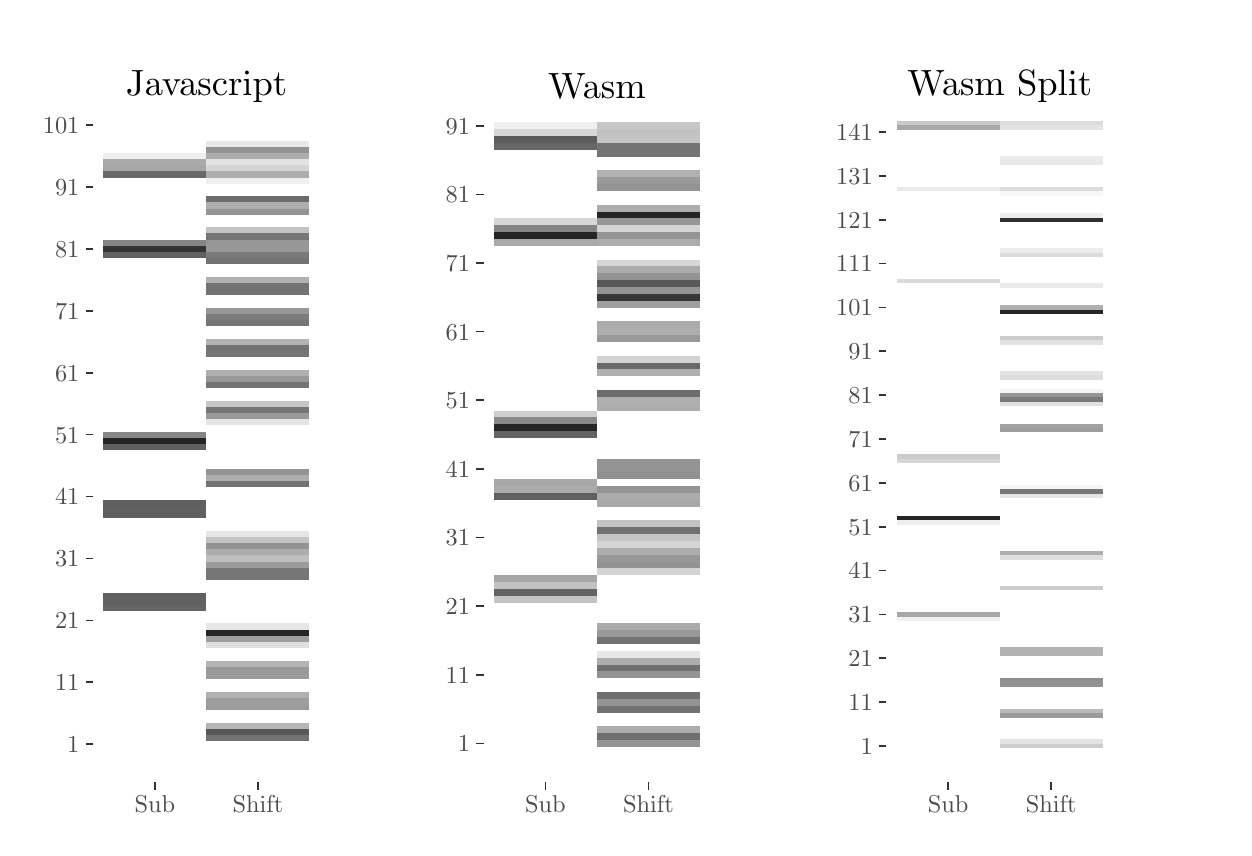
\begin{tikzpicture}[x=1pt,y=1pt]
\definecolor{fillColor}{RGB}{255,255,255}
\path[use as bounding box,fill=fillColor,fill opacity=0.00] (0,0) rectangle (432.17,289.08);
\begin{scope}
\path[clip] (  0.00,  0.00) rectangle (145.52,289.08);
\definecolor{drawColor}{RGB}{255,255,255}
\definecolor{fillColor}{RGB}{255,255,255}

\path[draw=drawColor,line width= 0.6pt,line join=round,line cap=round,fill=fillColor] (  0.00,  0.00) rectangle (145.52,289.08);
\end{scope}
\begin{scope}
\path[clip] (145.52,  0.00) rectangle (286.65,289.08);
\definecolor{drawColor}{RGB}{255,255,255}
\definecolor{fillColor}{RGB}{255,255,255}

\path[draw=drawColor,line width= 0.6pt,line join=round,line cap=round,fill=fillColor] (145.52,  0.00) rectangle (286.65,289.08);
\end{scope}
\begin{scope}
\path[clip] (286.65,  0.00) rectangle (432.17,289.08);
\definecolor{drawColor}{RGB}{255,255,255}
\definecolor{fillColor}{RGB}{255,255,255}

\path[draw=drawColor,line width= 0.6pt,line join=round,line cap=round,fill=fillColor] (286.65,  0.00) rectangle (432.17,289.08);
\end{scope}
\begin{scope}
\path[clip] ( 23.65, 16.51) rectangle (105.52,267.54);
\definecolor{drawColor}{RGB}{255,255,255}

\path[draw=drawColor,line width= 0.3pt,line join=round] ( 23.65, 18.97) --
	(105.52, 18.97);

\path[draw=drawColor,line width= 0.3pt,line join=round] ( 23.65, 41.35) --
	(105.52, 41.35);

\path[draw=drawColor,line width= 0.3pt,line join=round] ( 23.65, 63.72) --
	(105.52, 63.72);

\path[draw=drawColor,line width= 0.3pt,line join=round] ( 23.65, 86.09) --
	(105.52, 86.09);

\path[draw=drawColor,line width= 0.3pt,line join=round] ( 23.65,108.47) --
	(105.52,108.47);

\path[draw=drawColor,line width= 0.3pt,line join=round] ( 23.65,130.84) --
	(105.52,130.84);

\path[draw=drawColor,line width= 0.3pt,line join=round] ( 23.65,153.21) --
	(105.52,153.21);

\path[draw=drawColor,line width= 0.3pt,line join=round] ( 23.65,175.59) --
	(105.52,175.59);

\path[draw=drawColor,line width= 0.3pt,line join=round] ( 23.65,197.96) --
	(105.52,197.96);

\path[draw=drawColor,line width= 0.3pt,line join=round] ( 23.65,220.34) --
	(105.52,220.34);

\path[draw=drawColor,line width= 0.3pt,line join=round] ( 23.65,242.71) --
	(105.52,242.71);

\path[draw=drawColor,line width= 0.3pt,line join=round] ( 23.65,265.08) --
	(105.52,265.08);

\path[draw=drawColor,line width= 0.6pt,line join=round] ( 23.65, 30.16) --
	(105.52, 30.16);

\path[draw=drawColor,line width= 0.6pt,line join=round] ( 23.65, 52.53) --
	(105.52, 52.53);

\path[draw=drawColor,line width= 0.6pt,line join=round] ( 23.65, 74.91) --
	(105.52, 74.91);

\path[draw=drawColor,line width= 0.6pt,line join=round] ( 23.65, 97.28) --
	(105.52, 97.28);

\path[draw=drawColor,line width= 0.6pt,line join=round] ( 23.65,119.65) --
	(105.52,119.65);

\path[draw=drawColor,line width= 0.6pt,line join=round] ( 23.65,142.03) --
	(105.52,142.03);

\path[draw=drawColor,line width= 0.6pt,line join=round] ( 23.65,164.40) --
	(105.52,164.40);

\path[draw=drawColor,line width= 0.6pt,line join=round] ( 23.65,186.78) --
	(105.52,186.78);

\path[draw=drawColor,line width= 0.6pt,line join=round] ( 23.65,209.15) --
	(105.52,209.15);

\path[draw=drawColor,line width= 0.6pt,line join=round] ( 23.65,231.52) --
	(105.52,231.52);

\path[draw=drawColor,line width= 0.6pt,line join=round] ( 23.65,253.90) --
	(105.52,253.90);

\path[draw=drawColor,line width= 0.6pt,line join=round] ( 45.98, 16.51) --
	( 45.98,267.54);

\path[draw=drawColor,line width= 0.6pt,line join=round] ( 83.19, 16.51) --
	( 83.19,267.54);
\definecolor{fillColor}{RGB}{255,255,255}

\path[fill=fillColor] ( 27.37, 29.04) rectangle ( 64.59, 31.28);

\path[fill=fillColor] ( 27.37, 31.28) rectangle ( 64.59, 33.51);

\path[fill=fillColor] ( 27.37, 33.51) rectangle ( 64.59, 35.75);

\path[fill=fillColor] ( 27.37, 35.75) rectangle ( 64.59, 37.99);

\path[fill=fillColor] ( 27.37, 37.99) rectangle ( 64.59, 40.23);

\path[fill=fillColor] ( 27.37, 40.23) rectangle ( 64.59, 42.46);

\path[fill=fillColor] ( 27.37, 42.46) rectangle ( 64.59, 44.70);

\path[fill=fillColor] ( 27.37, 44.70) rectangle ( 64.59, 46.94);

\path[fill=fillColor] ( 27.37, 46.94) rectangle ( 64.59, 49.18);

\path[fill=fillColor] ( 27.37, 49.18) rectangle ( 64.59, 51.41);

\path[fill=fillColor] ( 27.37, 51.41) rectangle ( 64.59, 53.65);

\path[fill=fillColor] ( 27.37, 53.65) rectangle ( 64.59, 55.89);

\path[fill=fillColor] ( 27.37, 55.89) rectangle ( 64.59, 58.13);

\path[fill=fillColor] ( 27.37, 58.13) rectangle ( 64.59, 60.36);

\path[fill=fillColor] ( 27.37, 60.36) rectangle ( 64.59, 62.60);

\path[fill=fillColor] ( 27.37, 62.60) rectangle ( 64.59, 64.84);

\path[fill=fillColor] ( 27.37, 64.84) rectangle ( 64.59, 67.08);

\path[fill=fillColor] ( 27.37, 67.08) rectangle ( 64.59, 69.31);

\path[fill=fillColor] ( 27.37, 69.31) rectangle ( 64.59, 71.55);

\path[fill=fillColor] ( 27.37, 71.55) rectangle ( 64.59, 73.79);

\path[fill=fillColor] ( 27.37, 73.79) rectangle ( 64.59, 76.03);

\path[fill=fillColor] ( 27.37, 76.03) rectangle ( 64.59, 78.26);
\definecolor{fillColor}{RGB}{101,101,101}

\path[fill=fillColor] ( 27.37, 78.26) rectangle ( 64.59, 80.50);
\definecolor{fillColor}{gray}{0.38}

\path[fill=fillColor] ( 27.37, 80.50) rectangle ( 64.59, 82.74);

\path[fill=fillColor] ( 27.37, 82.74) rectangle ( 64.59, 84.97);
\definecolor{fillColor}{RGB}{255,255,255}

\path[fill=fillColor] ( 27.37, 84.97) rectangle ( 64.59, 87.21);

\path[fill=fillColor] ( 27.37, 87.21) rectangle ( 64.59, 89.45);

\path[fill=fillColor] ( 27.37, 89.45) rectangle ( 64.59, 91.69);

\path[fill=fillColor] ( 27.37, 91.69) rectangle ( 64.59, 93.92);

\path[fill=fillColor] ( 27.37, 93.92) rectangle ( 64.59, 96.16);

\path[fill=fillColor] ( 27.37, 96.16) rectangle ( 64.59, 98.40);

\path[fill=fillColor] ( 27.37, 98.40) rectangle ( 64.59,100.64);

\path[fill=fillColor] ( 27.37,100.64) rectangle ( 64.59,102.87);

\path[fill=fillColor] ( 27.37,102.87) rectangle ( 64.59,105.11);

\path[fill=fillColor] ( 27.37,105.11) rectangle ( 64.59,107.35);

\path[fill=fillColor] ( 27.37,107.35) rectangle ( 64.59,109.59);

\path[fill=fillColor] ( 27.37,109.59) rectangle ( 64.59,111.82);
\definecolor{fillColor}{RGB}{95,95,95}

\path[fill=fillColor] ( 27.37,111.82) rectangle ( 64.59,114.06);
\definecolor{fillColor}{gray}{0.38}

\path[fill=fillColor] ( 27.37,114.06) rectangle ( 64.59,116.30);
\definecolor{fillColor}{RGB}{95,95,95}

\path[fill=fillColor] ( 27.37,116.30) rectangle ( 64.59,118.54);
\definecolor{fillColor}{RGB}{255,255,255}

\path[fill=fillColor] ( 27.37,118.54) rectangle ( 64.59,120.77);

\path[fill=fillColor] ( 27.37,120.77) rectangle ( 64.59,123.01);

\path[fill=fillColor] ( 27.37,123.01) rectangle ( 64.59,125.25);

\path[fill=fillColor] ( 27.37,125.25) rectangle ( 64.59,127.48);

\path[fill=fillColor] ( 27.37,127.48) rectangle ( 64.59,129.72);

\path[fill=fillColor] ( 27.37,129.72) rectangle ( 64.59,131.96);

\path[fill=fillColor] ( 27.37,131.96) rectangle ( 64.59,134.20);

\path[fill=fillColor] ( 27.37,134.20) rectangle ( 64.59,136.43);
\definecolor{fillColor}{gray}{0.38}

\path[fill=fillColor] ( 27.37,136.43) rectangle ( 64.59,138.67);
\definecolor{fillColor}{RGB}{37,37,37}

\path[fill=fillColor] ( 27.37,138.67) rectangle ( 64.59,140.91);
\definecolor{fillColor}{RGB}{134,134,134}

\path[fill=fillColor] ( 27.37,140.91) rectangle ( 64.59,143.15);
\definecolor{fillColor}{RGB}{255,255,255}

\path[fill=fillColor] ( 27.37,143.15) rectangle ( 64.59,145.38);

\path[fill=fillColor] ( 27.37,145.38) rectangle ( 64.59,147.62);

\path[fill=fillColor] ( 27.37,147.62) rectangle ( 64.59,149.86);

\path[fill=fillColor] ( 27.37,149.86) rectangle ( 64.59,152.10);

\path[fill=fillColor] ( 27.37,152.10) rectangle ( 64.59,154.33);

\path[fill=fillColor] ( 27.37,154.33) rectangle ( 64.59,156.57);

\path[fill=fillColor] ( 27.37,156.57) rectangle ( 64.59,158.81);

\path[fill=fillColor] ( 27.37,158.81) rectangle ( 64.59,161.05);

\path[fill=fillColor] ( 27.37,161.05) rectangle ( 64.59,163.28);

\path[fill=fillColor] ( 27.37,163.28) rectangle ( 64.59,165.52);

\path[fill=fillColor] ( 27.37,165.52) rectangle ( 64.59,167.76);

\path[fill=fillColor] ( 27.37,167.76) rectangle ( 64.59,170.00);

\path[fill=fillColor] ( 27.37,170.00) rectangle ( 64.59,172.23);

\path[fill=fillColor] ( 27.37,172.23) rectangle ( 64.59,174.47);

\path[fill=fillColor] ( 27.37,174.47) rectangle ( 64.59,176.71);

\path[fill=fillColor] ( 27.37,176.71) rectangle ( 64.59,178.94);

\path[fill=fillColor] ( 27.37,178.94) rectangle ( 64.59,181.18);

\path[fill=fillColor] ( 27.37,181.18) rectangle ( 64.59,183.42);

\path[fill=fillColor] ( 27.37,183.42) rectangle ( 64.59,185.66);

\path[fill=fillColor] ( 27.37,185.66) rectangle ( 64.59,187.89);

\path[fill=fillColor] ( 27.37,187.89) rectangle ( 64.59,190.13);

\path[fill=fillColor] ( 27.37,190.13) rectangle ( 64.59,192.37);

\path[fill=fillColor] ( 27.37,192.37) rectangle ( 64.59,194.61);

\path[fill=fillColor] ( 27.37,194.61) rectangle ( 64.59,196.84);

\path[fill=fillColor] ( 27.37,196.84) rectangle ( 64.59,199.08);

\path[fill=fillColor] ( 27.37,199.08) rectangle ( 64.59,201.32);

\path[fill=fillColor] ( 27.37,201.32) rectangle ( 64.59,203.56);

\path[fill=fillColor] ( 27.37,203.56) rectangle ( 64.59,205.79);
\definecolor{fillColor}{gray}{0.38}

\path[fill=fillColor] ( 27.37,205.79) rectangle ( 64.59,208.03);
\definecolor{fillColor}{gray}{0.20}

\path[fill=fillColor] ( 27.37,208.03) rectangle ( 64.59,210.27);
\definecolor{fillColor}{gray}{0.52}

\path[fill=fillColor] ( 27.37,210.27) rectangle ( 64.59,212.51);
\definecolor{fillColor}{RGB}{255,255,255}

\path[fill=fillColor] ( 27.37,212.51) rectangle ( 64.59,214.74);

\path[fill=fillColor] ( 27.37,214.74) rectangle ( 64.59,216.98);

\path[fill=fillColor] ( 27.37,216.98) rectangle ( 64.59,219.22);

\path[fill=fillColor] ( 27.37,219.22) rectangle ( 64.59,221.45);

\path[fill=fillColor] ( 27.37,221.45) rectangle ( 64.59,223.69);

\path[fill=fillColor] ( 27.37,223.69) rectangle ( 64.59,225.93);

\path[fill=fillColor] ( 27.37,225.93) rectangle ( 64.59,228.17);

\path[fill=fillColor] ( 27.37,228.17) rectangle ( 64.59,230.40);

\path[fill=fillColor] ( 27.37,230.40) rectangle ( 64.59,232.64);

\path[fill=fillColor] ( 27.37,232.64) rectangle ( 64.59,234.88);
\definecolor{fillColor}{RGB}{105,105,105}

\path[fill=fillColor] ( 27.37,234.88) rectangle ( 64.59,237.12);
\definecolor{fillColor}{gray}{0.65}

\path[fill=fillColor] ( 27.37,237.12) rectangle ( 64.59,239.35);
\definecolor{fillColor}{RGB}{169,169,169}

\path[fill=fillColor] ( 27.37,239.35) rectangle ( 64.59,241.59);
\definecolor{fillColor}{RGB}{238,238,238}

\path[fill=fillColor] ( 27.37,241.59) rectangle ( 64.59,243.83);
\definecolor{fillColor}{RGB}{255,255,255}

\path[fill=fillColor] ( 27.37,243.83) rectangle ( 64.59,246.07);

\path[fill=fillColor] ( 27.37,246.07) rectangle ( 64.59,248.30);

\path[fill=fillColor] ( 27.37,248.30) rectangle ( 64.59,250.54);

\path[fill=fillColor] ( 27.37,250.54) rectangle ( 64.59,252.78);

\path[fill=fillColor] ( 27.37,252.78) rectangle ( 64.59,255.02);

\path[fill=fillColor] ( 64.59, 29.04) rectangle (101.80, 31.28);
\definecolor{fillColor}{RGB}{114,114,114}

\path[fill=fillColor] ( 64.59, 31.28) rectangle (101.80, 33.51);
\definecolor{fillColor}{RGB}{88,88,88}

\path[fill=fillColor] ( 64.59, 33.51) rectangle (101.80, 35.75);
\definecolor{fillColor}{gray}{0.71}

\path[fill=fillColor] ( 64.59, 35.75) rectangle (101.80, 37.99);
\definecolor{fillColor}{RGB}{255,255,255}

\path[fill=fillColor] ( 64.59, 37.99) rectangle (101.80, 40.23);

\path[fill=fillColor] ( 64.59, 40.23) rectangle (101.80, 42.46);
\definecolor{fillColor}{RGB}{155,155,155}

\path[fill=fillColor] ( 64.59, 42.46) rectangle (101.80, 44.70);
\definecolor{fillColor}{gray}{0.62}

\path[fill=fillColor] ( 64.59, 44.70) rectangle (101.80, 46.94);
\definecolor{fillColor}{RGB}{177,177,177}

\path[fill=fillColor] ( 64.59, 46.94) rectangle (101.80, 49.18);
\definecolor{fillColor}{RGB}{255,255,255}

\path[fill=fillColor] ( 64.59, 49.18) rectangle (101.80, 51.41);

\path[fill=fillColor] ( 64.59, 51.41) rectangle (101.80, 53.65);
\definecolor{fillColor}{RGB}{155,155,155}

\path[fill=fillColor] ( 64.59, 53.65) rectangle (101.80, 55.89);
\definecolor{fillColor}{gray}{0.60}

\path[fill=fillColor] ( 64.59, 55.89) rectangle (101.80, 58.13);
\definecolor{fillColor}{RGB}{180,180,180}

\path[fill=fillColor] ( 64.59, 58.13) rectangle (101.80, 60.36);
\definecolor{fillColor}{RGB}{255,255,255}

\path[fill=fillColor] ( 64.59, 60.36) rectangle (101.80, 62.60);

\path[fill=fillColor] ( 64.59, 62.60) rectangle (101.80, 64.84);
\definecolor{fillColor}{RGB}{223,223,223}

\path[fill=fillColor] ( 64.59, 64.84) rectangle (101.80, 67.08);
\definecolor{fillColor}{gray}{0.62}

\path[fill=fillColor] ( 64.59, 67.08) rectangle (101.80, 69.31);
\definecolor{fillColor}{RGB}{37,37,37}

\path[fill=fillColor] ( 64.59, 69.31) rectangle (101.80, 71.55);
\definecolor{fillColor}{RGB}{230,230,230}

\path[fill=fillColor] ( 64.59, 71.55) rectangle (101.80, 73.79);
\definecolor{fillColor}{RGB}{255,255,255}

\path[fill=fillColor] ( 64.59, 73.79) rectangle (101.80, 76.03);

\path[fill=fillColor] ( 64.59, 76.03) rectangle (101.80, 78.26);

\path[fill=fillColor] ( 64.59, 78.26) rectangle (101.80, 80.50);

\path[fill=fillColor] ( 64.59, 80.50) rectangle (101.80, 82.74);

\path[fill=fillColor] ( 64.59, 82.74) rectangle (101.80, 84.97);

\path[fill=fillColor] ( 64.59, 84.97) rectangle (101.80, 87.21);

\path[fill=fillColor] ( 64.59, 87.21) rectangle (101.80, 89.45);
\definecolor{fillColor}{RGB}{118,118,118}

\path[fill=fillColor] ( 64.59, 89.45) rectangle (101.80, 91.69);

\path[fill=fillColor] ( 64.59, 91.69) rectangle (101.80, 93.92);
\definecolor{fillColor}{RGB}{155,155,155}

\path[fill=fillColor] ( 64.59, 93.92) rectangle (101.80, 96.16);
\definecolor{fillColor}{gray}{0.75}

\path[fill=fillColor] ( 64.59, 96.16) rectangle (101.80, 98.40);
\definecolor{fillColor}{gray}{0.68}

\path[fill=fillColor] ( 64.59, 98.40) rectangle (101.80,100.64);
\definecolor{fillColor}{RGB}{147,147,147}

\path[fill=fillColor] ( 64.59,100.64) rectangle (101.80,102.87);
\definecolor{fillColor}{gray}{0.77}

\path[fill=fillColor] ( 64.59,102.87) rectangle (101.80,105.11);
\definecolor{fillColor}{RGB}{230,230,230}

\path[fill=fillColor] ( 64.59,105.11) rectangle (101.80,107.35);
\definecolor{fillColor}{RGB}{255,255,255}

\path[fill=fillColor] ( 64.59,107.35) rectangle (101.80,109.59);

\path[fill=fillColor] ( 64.59,109.59) rectangle (101.80,111.82);

\path[fill=fillColor] ( 64.59,111.82) rectangle (101.80,114.06);

\path[fill=fillColor] ( 64.59,114.06) rectangle (101.80,116.30);

\path[fill=fillColor] ( 64.59,116.30) rectangle (101.80,118.54);

\path[fill=fillColor] ( 64.59,118.54) rectangle (101.80,120.77);

\path[fill=fillColor] ( 64.59,120.77) rectangle (101.80,123.01);
\definecolor{fillColor}{gray}{0.45}

\path[fill=fillColor] ( 64.59,123.01) rectangle (101.80,125.25);
\definecolor{fillColor}{RGB}{174,174,174}

\path[fill=fillColor] ( 64.59,125.25) rectangle (101.80,127.48);
\definecolor{fillColor}{gray}{0.58}

\path[fill=fillColor] ( 64.59,127.48) rectangle (101.80,129.72);
\definecolor{fillColor}{RGB}{255,255,255}

\path[fill=fillColor] ( 64.59,129.72) rectangle (101.80,131.96);

\path[fill=fillColor] ( 64.59,131.96) rectangle (101.80,134.20);

\path[fill=fillColor] ( 64.59,134.20) rectangle (101.80,136.43);

\path[fill=fillColor] ( 64.59,136.43) rectangle (101.80,138.67);

\path[fill=fillColor] ( 64.59,138.67) rectangle (101.80,140.91);

\path[fill=fillColor] ( 64.59,140.91) rectangle (101.80,143.15);

\path[fill=fillColor] ( 64.59,143.15) rectangle (101.80,145.38);
\definecolor{fillColor}{RGB}{228,228,228}

\path[fill=fillColor] ( 64.59,145.38) rectangle (101.80,147.62);
\definecolor{fillColor}{RGB}{154,154,154}

\path[fill=fillColor] ( 64.59,147.62) rectangle (101.80,149.86);
\definecolor{fillColor}{RGB}{118,118,118}

\path[fill=fillColor] ( 64.59,149.86) rectangle (101.80,152.10);
\definecolor{fillColor}{gray}{0.78}

\path[fill=fillColor] ( 64.59,152.10) rectangle (101.80,154.33);
\definecolor{fillColor}{RGB}{255,255,255}

\path[fill=fillColor] ( 64.59,154.33) rectangle (101.80,156.57);

\path[fill=fillColor] ( 64.59,156.57) rectangle (101.80,158.81);
\definecolor{fillColor}{RGB}{116,116,116}

\path[fill=fillColor] ( 64.59,158.81) rectangle (101.80,161.05);
\definecolor{fillColor}{gray}{0.60}

\path[fill=fillColor] ( 64.59,161.05) rectangle (101.80,163.28);
\definecolor{fillColor}{RGB}{175,175,175}

\path[fill=fillColor] ( 64.59,163.28) rectangle (101.80,165.52);
\definecolor{fillColor}{RGB}{255,255,255}

\path[fill=fillColor] ( 64.59,165.52) rectangle (101.80,167.76);

\path[fill=fillColor] ( 64.59,167.76) rectangle (101.80,170.00);
\definecolor{fillColor}{RGB}{118,118,118}

\path[fill=fillColor] ( 64.59,170.00) rectangle (101.80,172.23);
\definecolor{fillColor}{gray}{0.45}

\path[fill=fillColor] ( 64.59,172.23) rectangle (101.80,174.47);
\definecolor{fillColor}{RGB}{178,178,178}

\path[fill=fillColor] ( 64.59,174.47) rectangle (101.80,176.71);
\definecolor{fillColor}{RGB}{255,255,255}

\path[fill=fillColor] ( 64.59,176.71) rectangle (101.80,178.94);

\path[fill=fillColor] ( 64.59,178.94) rectangle (101.80,181.18);
\definecolor{fillColor}{gray}{0.46}

\path[fill=fillColor] ( 64.59,181.18) rectangle (101.80,183.42);
\definecolor{fillColor}{RGB}{123,123,123}

\path[fill=fillColor] ( 64.59,183.42) rectangle (101.80,185.66);
\definecolor{fillColor}{RGB}{151,151,151}

\path[fill=fillColor] ( 64.59,185.66) rectangle (101.80,187.89);
\definecolor{fillColor}{RGB}{255,255,255}

\path[fill=fillColor] ( 64.59,187.89) rectangle (101.80,190.13);

\path[fill=fillColor] ( 64.59,190.13) rectangle (101.80,192.37);
\definecolor{fillColor}{gray}{0.45}

\path[fill=fillColor] ( 64.59,192.37) rectangle (101.80,194.61);

\path[fill=fillColor] ( 64.59,194.61) rectangle (101.80,196.84);
\definecolor{fillColor}{RGB}{177,177,177}

\path[fill=fillColor] ( 64.59,196.84) rectangle (101.80,199.08);
\definecolor{fillColor}{RGB}{255,255,255}

\path[fill=fillColor] ( 64.59,199.08) rectangle (101.80,201.32);

\path[fill=fillColor] ( 64.59,201.32) rectangle (101.80,203.56);
\definecolor{fillColor}{gray}{0.45}

\path[fill=fillColor] ( 64.59,203.56) rectangle (101.80,205.79);
\definecolor{fillColor}{gray}{0.48}

\path[fill=fillColor] ( 64.59,205.79) rectangle (101.80,208.03);
\definecolor{fillColor}{RGB}{152,152,152}

\path[fill=fillColor] ( 64.59,208.03) rectangle (101.80,210.27);
\definecolor{fillColor}{RGB}{151,151,151}

\path[fill=fillColor] ( 64.59,210.27) rectangle (101.80,212.51);
\definecolor{fillColor}{RGB}{118,118,118}

\path[fill=fillColor] ( 64.59,212.51) rectangle (101.80,214.74);
\definecolor{fillColor}{gray}{0.77}

\path[fill=fillColor] ( 64.59,214.74) rectangle (101.80,216.98);
\definecolor{fillColor}{RGB}{255,255,255}

\path[fill=fillColor] ( 64.59,216.98) rectangle (101.80,219.22);

\path[fill=fillColor] ( 64.59,219.22) rectangle (101.80,221.45);
\definecolor{fillColor}{gray}{0.58}

\path[fill=fillColor] ( 64.59,221.45) rectangle (101.80,223.69);
\definecolor{fillColor}{RGB}{174,174,174}

\path[fill=fillColor] ( 64.59,223.69) rectangle (101.80,225.93);
\definecolor{fillColor}{RGB}{109,109,109}

\path[fill=fillColor] ( 64.59,225.93) rectangle (101.80,228.17);
\definecolor{fillColor}{RGB}{255,255,255}

\path[fill=fillColor] ( 64.59,228.17) rectangle (101.80,230.40);

\path[fill=fillColor] ( 64.59,230.40) rectangle (101.80,232.64);
\definecolor{fillColor}{RGB}{239,239,239}

\path[fill=fillColor] ( 64.59,232.64) rectangle (101.80,234.88);
\definecolor{fillColor}{RGB}{174,174,174}

\path[fill=fillColor] ( 64.59,234.88) rectangle (101.80,237.12);
\definecolor{fillColor}{RGB}{213,213,213}

\path[fill=fillColor] ( 64.59,237.12) rectangle (101.80,239.35);
\definecolor{fillColor}{gray}{0.89}

\path[fill=fillColor] ( 64.59,239.35) rectangle (101.80,241.59);
\definecolor{fillColor}{RGB}{172,172,172}

\path[fill=fillColor] ( 64.59,241.59) rectangle (101.80,243.83);
\definecolor{fillColor}{RGB}{147,147,147}

\path[fill=fillColor] ( 64.59,243.83) rectangle (101.80,246.07);
\definecolor{fillColor}{gray}{0.91}

\path[fill=fillColor] ( 64.59,246.07) rectangle (101.80,248.30);
\definecolor{fillColor}{RGB}{255,255,255}

\path[fill=fillColor] ( 64.59,248.30) rectangle (101.80,250.54);

\path[fill=fillColor] ( 64.59,250.54) rectangle (101.80,252.78);

\path[fill=fillColor] ( 64.59,252.78) rectangle (101.80,255.02);
\end{scope}
\begin{scope}
\path[clip] (164.77, 16.51) rectangle (246.65,267.54);
\definecolor{drawColor}{RGB}{255,255,255}

\path[draw=drawColor,line width= 0.3pt,line join=round] (164.77, 18.00) --
	(246.65, 18.00);

\path[draw=drawColor,line width= 0.3pt,line join=round] (164.77, 42.80) --
	(246.65, 42.80);

\path[draw=drawColor,line width= 0.3pt,line join=round] (164.77, 67.61) --
	(246.65, 67.61);

\path[draw=drawColor,line width= 0.3pt,line join=round] (164.77, 92.42) --
	(246.65, 92.42);

\path[draw=drawColor,line width= 0.3pt,line join=round] (164.77,117.22) --
	(246.65,117.22);

\path[draw=drawColor,line width= 0.3pt,line join=round] (164.77,142.03) --
	(246.65,142.03);

\path[draw=drawColor,line width= 0.3pt,line join=round] (164.77,166.83) --
	(246.65,166.83);

\path[draw=drawColor,line width= 0.3pt,line join=round] (164.77,191.64) --
	(246.65,191.64);

\path[draw=drawColor,line width= 0.3pt,line join=round] (164.77,216.45) --
	(246.65,216.45);

\path[draw=drawColor,line width= 0.3pt,line join=round] (164.77,241.25) --
	(246.65,241.25);

\path[draw=drawColor,line width= 0.3pt,line join=round] (164.77,266.06) --
	(246.65,266.06);

\path[draw=drawColor,line width= 0.6pt,line join=round] (164.77, 30.40) --
	(246.65, 30.40);

\path[draw=drawColor,line width= 0.6pt,line join=round] (164.77, 55.21) --
	(246.65, 55.21);

\path[draw=drawColor,line width= 0.6pt,line join=round] (164.77, 80.01) --
	(246.65, 80.01);

\path[draw=drawColor,line width= 0.6pt,line join=round] (164.77,104.82) --
	(246.65,104.82);

\path[draw=drawColor,line width= 0.6pt,line join=round] (164.77,129.62) --
	(246.65,129.62);

\path[draw=drawColor,line width= 0.6pt,line join=round] (164.77,154.43) --
	(246.65,154.43);

\path[draw=drawColor,line width= 0.6pt,line join=round] (164.77,179.24) --
	(246.65,179.24);

\path[draw=drawColor,line width= 0.6pt,line join=round] (164.77,204.04) --
	(246.65,204.04);

\path[draw=drawColor,line width= 0.6pt,line join=round] (164.77,228.85) --
	(246.65,228.85);

\path[draw=drawColor,line width= 0.6pt,line join=round] (164.77,253.65) --
	(246.65,253.65);

\path[draw=drawColor,line width= 0.6pt,line join=round] (187.10, 16.51) --
	(187.10,267.54);

\path[draw=drawColor,line width= 0.6pt,line join=round] (224.32, 16.51) --
	(224.32,267.54);
\definecolor{fillColor}{RGB}{255,255,255}

\path[fill=fillColor] (168.49, 29.16) rectangle (205.71, 31.64);

\path[fill=fillColor] (168.49, 31.64) rectangle (205.71, 34.12);

\path[fill=fillColor] (168.49, 34.12) rectangle (205.71, 36.60);

\path[fill=fillColor] (168.49, 36.60) rectangle (205.71, 39.08);

\path[fill=fillColor] (168.49, 39.08) rectangle (205.71, 41.56);

\path[fill=fillColor] (168.49, 41.56) rectangle (205.71, 44.05);

\path[fill=fillColor] (168.49, 44.05) rectangle (205.71, 46.53);

\path[fill=fillColor] (168.49, 46.53) rectangle (205.71, 49.01);

\path[fill=fillColor] (168.49, 49.01) rectangle (205.71, 51.49);

\path[fill=fillColor] (168.49, 51.49) rectangle (205.71, 53.97);

\path[fill=fillColor] (168.49, 53.97) rectangle (205.71, 56.45);

\path[fill=fillColor] (168.49, 56.45) rectangle (205.71, 58.93);

\path[fill=fillColor] (168.49, 58.93) rectangle (205.71, 61.41);

\path[fill=fillColor] (168.49, 61.41) rectangle (205.71, 63.89);

\path[fill=fillColor] (168.49, 63.89) rectangle (205.71, 66.37);

\path[fill=fillColor] (168.49, 66.37) rectangle (205.71, 68.85);

\path[fill=fillColor] (168.49, 68.85) rectangle (205.71, 71.33);

\path[fill=fillColor] (168.49, 71.33) rectangle (205.71, 73.81);

\path[fill=fillColor] (168.49, 73.81) rectangle (205.71, 76.29);

\path[fill=fillColor] (168.49, 76.29) rectangle (205.71, 78.77);

\path[fill=fillColor] (168.49, 78.77) rectangle (205.71, 81.25);
\definecolor{fillColor}{gray}{0.77}

\path[fill=fillColor] (168.49, 81.25) rectangle (205.71, 83.73);
\definecolor{fillColor}{gray}{0.39}

\path[fill=fillColor] (168.49, 83.73) rectangle (205.71, 86.21);
\definecolor{fillColor}{gray}{0.76}

\path[fill=fillColor] (168.49, 86.21) rectangle (205.71, 88.70);
\definecolor{fillColor}{gray}{0.65}

\path[fill=fillColor] (168.49, 88.70) rectangle (205.71, 91.18);
\definecolor{fillColor}{RGB}{255,255,255}

\path[fill=fillColor] (168.49, 91.18) rectangle (205.71, 93.66);

\path[fill=fillColor] (168.49, 93.66) rectangle (205.71, 96.14);

\path[fill=fillColor] (168.49, 96.14) rectangle (205.71, 98.62);

\path[fill=fillColor] (168.49, 98.62) rectangle (205.71,101.10);

\path[fill=fillColor] (168.49,101.10) rectangle (205.71,103.58);

\path[fill=fillColor] (168.49,103.58) rectangle (205.71,106.06);

\path[fill=fillColor] (168.49,106.06) rectangle (205.71,108.54);

\path[fill=fillColor] (168.49,108.54) rectangle (205.71,111.02);

\path[fill=fillColor] (168.49,111.02) rectangle (205.71,113.50);

\path[fill=fillColor] (168.49,113.50) rectangle (205.71,115.98);

\path[fill=fillColor] (168.49,115.98) rectangle (205.71,118.46);
\definecolor{fillColor}{RGB}{96,96,96}

\path[fill=fillColor] (168.49,118.46) rectangle (205.71,120.94);
\definecolor{fillColor}{gray}{0.67}

\path[fill=fillColor] (168.49,120.94) rectangle (205.71,123.42);
\definecolor{fillColor}{gray}{0.66}

\path[fill=fillColor] (168.49,123.42) rectangle (205.71,125.90);
\definecolor{fillColor}{RGB}{255,255,255}

\path[fill=fillColor] (168.49,125.90) rectangle (205.71,128.38);

\path[fill=fillColor] (168.49,128.38) rectangle (205.71,130.87);

\path[fill=fillColor] (168.49,130.87) rectangle (205.71,133.35);

\path[fill=fillColor] (168.49,133.35) rectangle (205.71,135.83);

\path[fill=fillColor] (168.49,135.83) rectangle (205.71,138.31);

\path[fill=fillColor] (168.49,138.31) rectangle (205.71,140.79);
\definecolor{fillColor}{gray}{0.39}

\path[fill=fillColor] (168.49,140.79) rectangle (205.71,143.27);
\definecolor{fillColor}{RGB}{37,37,37}

\path[fill=fillColor] (168.49,143.27) rectangle (205.71,145.75);
\definecolor{fillColor}{RGB}{137,137,137}

\path[fill=fillColor] (168.49,145.75) rectangle (205.71,148.23);
\definecolor{fillColor}{RGB}{206,206,206}

\path[fill=fillColor] (168.49,148.23) rectangle (205.71,150.71);
\definecolor{fillColor}{RGB}{255,255,255}

\path[fill=fillColor] (168.49,150.71) rectangle (205.71,153.19);

\path[fill=fillColor] (168.49,153.19) rectangle (205.71,155.67);

\path[fill=fillColor] (168.49,155.67) rectangle (205.71,158.15);

\path[fill=fillColor] (168.49,158.15) rectangle (205.71,160.63);

\path[fill=fillColor] (168.49,160.63) rectangle (205.71,163.11);

\path[fill=fillColor] (168.49,163.11) rectangle (205.71,165.59);

\path[fill=fillColor] (168.49,165.59) rectangle (205.71,168.07);

\path[fill=fillColor] (168.49,168.07) rectangle (205.71,170.55);

\path[fill=fillColor] (168.49,170.55) rectangle (205.71,173.04);

\path[fill=fillColor] (168.49,173.04) rectangle (205.71,175.52);

\path[fill=fillColor] (168.49,175.52) rectangle (205.71,178.00);

\path[fill=fillColor] (168.49,178.00) rectangle (205.71,180.48);

\path[fill=fillColor] (168.49,180.48) rectangle (205.71,182.96);

\path[fill=fillColor] (168.49,182.96) rectangle (205.71,185.44);

\path[fill=fillColor] (168.49,185.44) rectangle (205.71,187.92);

\path[fill=fillColor] (168.49,187.92) rectangle (205.71,190.40);

\path[fill=fillColor] (168.49,190.40) rectangle (205.71,192.88);

\path[fill=fillColor] (168.49,192.88) rectangle (205.71,195.36);

\path[fill=fillColor] (168.49,195.36) rectangle (205.71,197.84);

\path[fill=fillColor] (168.49,197.84) rectangle (205.71,200.32);

\path[fill=fillColor] (168.49,200.32) rectangle (205.71,202.80);

\path[fill=fillColor] (168.49,202.80) rectangle (205.71,205.28);

\path[fill=fillColor] (168.49,205.28) rectangle (205.71,207.76);

\path[fill=fillColor] (168.49,207.76) rectangle (205.71,210.24);
\definecolor{fillColor}{RGB}{169,169,169}

\path[fill=fillColor] (168.49,210.24) rectangle (205.71,212.72);
\definecolor{fillColor}{RGB}{37,37,37}

\path[fill=fillColor] (168.49,212.72) rectangle (205.71,215.20);
\definecolor{fillColor}{gray}{0.52}

\path[fill=fillColor] (168.49,215.20) rectangle (205.71,217.69);
\definecolor{fillColor}{gray}{0.84}

\path[fill=fillColor] (168.49,217.69) rectangle (205.71,220.17);
\definecolor{fillColor}{RGB}{255,255,255}

\path[fill=fillColor] (168.49,220.17) rectangle (205.71,222.65);

\path[fill=fillColor] (168.49,222.65) rectangle (205.71,225.13);

\path[fill=fillColor] (168.49,225.13) rectangle (205.71,227.61);

\path[fill=fillColor] (168.49,227.61) rectangle (205.71,230.09);

\path[fill=fillColor] (168.49,230.09) rectangle (205.71,232.57);

\path[fill=fillColor] (168.49,232.57) rectangle (205.71,235.05);

\path[fill=fillColor] (168.49,235.05) rectangle (205.71,237.53);

\path[fill=fillColor] (168.49,237.53) rectangle (205.71,240.01);

\path[fill=fillColor] (168.49,240.01) rectangle (205.71,242.49);

\path[fill=fillColor] (168.49,242.49) rectangle (205.71,244.97);
\definecolor{fillColor}{RGB}{103,103,103}

\path[fill=fillColor] (168.49,244.97) rectangle (205.71,247.45);
\definecolor{fillColor}{gray}{0.36}

\path[fill=fillColor] (168.49,247.45) rectangle (205.71,249.93);
\definecolor{fillColor}{RGB}{215,215,215}

\path[fill=fillColor] (168.49,249.93) rectangle (205.71,252.41);
\definecolor{fillColor}{RGB}{239,239,239}

\path[fill=fillColor] (168.49,252.41) rectangle (205.71,254.89);
\definecolor{fillColor}{gray}{0.58}

\path[fill=fillColor] (205.71, 29.16) rectangle (242.93, 31.64);
\definecolor{fillColor}{RGB}{111,111,111}

\path[fill=fillColor] (205.71, 31.64) rectangle (242.93, 34.12);
\definecolor{fillColor}{gray}{0.68}

\path[fill=fillColor] (205.71, 34.12) rectangle (242.93, 36.60);
\definecolor{fillColor}{RGB}{255,255,255}

\path[fill=fillColor] (205.71, 36.60) rectangle (242.93, 39.08);

\path[fill=fillColor] (205.71, 39.08) rectangle (242.93, 41.56);
\definecolor{fillColor}{RGB}{114,114,114}

\path[fill=fillColor] (205.71, 41.56) rectangle (242.93, 44.05);
\definecolor{fillColor}{gray}{0.58}

\path[fill=fillColor] (205.71, 44.05) rectangle (242.93, 46.53);
\definecolor{fillColor}{gray}{0.44}

\path[fill=fillColor] (205.71, 46.53) rectangle (242.93, 49.01);
\definecolor{fillColor}{RGB}{255,255,255}

\path[fill=fillColor] (205.71, 49.01) rectangle (242.93, 51.49);

\path[fill=fillColor] (205.71, 51.49) rectangle (242.93, 53.97);
\definecolor{fillColor}{RGB}{147,147,147}

\path[fill=fillColor] (205.71, 53.97) rectangle (242.93, 56.45);
\definecolor{fillColor}{gray}{0.44}

\path[fill=fillColor] (205.71, 56.45) rectangle (242.93, 58.93);
\definecolor{fillColor}{gray}{0.68}

\path[fill=fillColor] (205.71, 58.93) rectangle (242.93, 61.41);
\definecolor{fillColor}{gray}{0.91}

\path[fill=fillColor] (205.71, 61.41) rectangle (242.93, 63.89);
\definecolor{fillColor}{RGB}{255,255,255}

\path[fill=fillColor] (205.71, 63.89) rectangle (242.93, 66.37);
\definecolor{fillColor}{RGB}{114,114,114}

\path[fill=fillColor] (205.71, 66.37) rectangle (242.93, 68.85);
\definecolor{fillColor}{RGB}{152,152,152}

\path[fill=fillColor] (205.71, 68.85) rectangle (242.93, 71.33);
\definecolor{fillColor}{RGB}{170,170,170}

\path[fill=fillColor] (205.71, 71.33) rectangle (242.93, 73.81);
\definecolor{fillColor}{RGB}{255,255,255}

\path[fill=fillColor] (205.71, 73.81) rectangle (242.93, 76.29);

\path[fill=fillColor] (205.71, 76.29) rectangle (242.93, 78.77);

\path[fill=fillColor] (205.71, 78.77) rectangle (242.93, 81.25);

\path[fill=fillColor] (205.71, 81.25) rectangle (242.93, 83.73);

\path[fill=fillColor] (205.71, 83.73) rectangle (242.93, 86.21);

\path[fill=fillColor] (205.71, 86.21) rectangle (242.93, 88.70);

\path[fill=fillColor] (205.71, 88.70) rectangle (242.93, 91.18);
\definecolor{fillColor}{RGB}{211,211,211}

\path[fill=fillColor] (205.71, 91.18) rectangle (242.93, 93.66);
\definecolor{fillColor}{RGB}{147,147,147}

\path[fill=fillColor] (205.71, 93.66) rectangle (242.93, 96.14);
\definecolor{fillColor}{RGB}{152,152,152}

\path[fill=fillColor] (205.71, 96.14) rectangle (242.93, 98.62);
\definecolor{fillColor}{gray}{0.68}

\path[fill=fillColor] (205.71, 98.62) rectangle (242.93,101.10);
\definecolor{fillColor}{RGB}{213,213,213}

\path[fill=fillColor] (205.71,101.10) rectangle (242.93,103.58);
\definecolor{fillColor}{gray}{0.77}

\path[fill=fillColor] (205.71,103.58) rectangle (242.93,106.06);
\definecolor{fillColor}{RGB}{113,113,113}

\path[fill=fillColor] (205.71,106.06) rectangle (242.93,108.54);
\definecolor{fillColor}{RGB}{195,195,195}

\path[fill=fillColor] (205.71,108.54) rectangle (242.93,111.02);
\definecolor{fillColor}{RGB}{255,255,255}

\path[fill=fillColor] (205.71,111.02) rectangle (242.93,113.50);

\path[fill=fillColor] (205.71,113.50) rectangle (242.93,115.98);
\definecolor{fillColor}{RGB}{169,169,169}

\path[fill=fillColor] (205.71,115.98) rectangle (242.93,118.46);
\definecolor{fillColor}{RGB}{172,172,172}

\path[fill=fillColor] (205.71,118.46) rectangle (242.93,120.94);
\definecolor{fillColor}{gray}{0.58}

\path[fill=fillColor] (205.71,120.94) rectangle (242.93,123.42);
\definecolor{fillColor}{RGB}{255,255,255}

\path[fill=fillColor] (205.71,123.42) rectangle (242.93,125.90);
\definecolor{fillColor}{gray}{0.57}

\path[fill=fillColor] (205.71,125.90) rectangle (242.93,128.38);
\definecolor{fillColor}{gray}{0.58}

\path[fill=fillColor] (205.71,128.38) rectangle (242.93,130.87);

\path[fill=fillColor] (205.71,130.87) rectangle (242.93,133.35);
\definecolor{fillColor}{RGB}{255,255,255}

\path[fill=fillColor] (205.71,133.35) rectangle (242.93,135.83);

\path[fill=fillColor] (205.71,135.83) rectangle (242.93,138.31);

\path[fill=fillColor] (205.71,138.31) rectangle (242.93,140.79);

\path[fill=fillColor] (205.71,140.79) rectangle (242.93,143.27);

\path[fill=fillColor] (205.71,143.27) rectangle (242.93,145.75);

\path[fill=fillColor] (205.71,145.75) rectangle (242.93,148.23);

\path[fill=fillColor] (205.71,148.23) rectangle (242.93,150.71);
\definecolor{fillColor}{gray}{0.68}

\path[fill=fillColor] (205.71,150.71) rectangle (242.93,153.19);
\definecolor{fillColor}{RGB}{175,175,175}

\path[fill=fillColor] (205.71,153.19) rectangle (242.93,155.67);
\definecolor{fillColor}{RGB}{108,108,108}

\path[fill=fillColor] (205.71,155.67) rectangle (242.93,158.15);
\definecolor{fillColor}{RGB}{255,255,255}

\path[fill=fillColor] (205.71,158.15) rectangle (242.93,160.63);

\path[fill=fillColor] (205.71,160.63) rectangle (242.93,163.11);
\definecolor{fillColor}{gray}{0.69}

\path[fill=fillColor] (205.71,163.11) rectangle (242.93,165.59);
\definecolor{fillColor}{RGB}{106,106,106}

\path[fill=fillColor] (205.71,165.59) rectangle (242.93,168.07);
\definecolor{fillColor}{RGB}{211,211,211}

\path[fill=fillColor] (205.71,168.07) rectangle (242.93,170.55);
\definecolor{fillColor}{RGB}{255,255,255}

\path[fill=fillColor] (205.71,170.55) rectangle (242.93,173.04);

\path[fill=fillColor] (205.71,173.04) rectangle (242.93,175.52);
\definecolor{fillColor}{gray}{0.60}

\path[fill=fillColor] (205.71,175.52) rectangle (242.93,178.00);
\definecolor{fillColor}{RGB}{174,174,174}

\path[fill=fillColor] (205.71,178.00) rectangle (242.93,180.48);
\definecolor{fillColor}{RGB}{172,172,172}

\path[fill=fillColor] (205.71,180.48) rectangle (242.93,182.96);
\definecolor{fillColor}{RGB}{255,255,255}

\path[fill=fillColor] (205.71,182.96) rectangle (242.93,185.44);

\path[fill=fillColor] (205.71,185.44) rectangle (242.93,187.92);
\definecolor{fillColor}{RGB}{159,159,159}

\path[fill=fillColor] (205.71,187.92) rectangle (242.93,190.40);
\definecolor{fillColor}{RGB}{55,55,55}

\path[fill=fillColor] (205.71,190.40) rectangle (242.93,192.88);
\definecolor{fillColor}{gray}{0.58}

\path[fill=fillColor] (205.71,192.88) rectangle (242.93,195.36);
\definecolor{fillColor}{RGB}{88,88,88}

\path[fill=fillColor] (205.71,195.36) rectangle (242.93,197.84);
\definecolor{fillColor}{RGB}{147,147,147}

\path[fill=fillColor] (205.71,197.84) rectangle (242.93,200.32);
\definecolor{fillColor}{RGB}{172,172,172}

\path[fill=fillColor] (205.71,200.32) rectangle (242.93,202.80);
\definecolor{fillColor}{gray}{0.84}

\path[fill=fillColor] (205.71,202.80) rectangle (242.93,205.28);
\definecolor{fillColor}{RGB}{255,255,255}

\path[fill=fillColor] (205.71,205.28) rectangle (242.93,207.76);

\path[fill=fillColor] (205.71,207.76) rectangle (242.93,210.24);
\definecolor{fillColor}{gray}{0.68}

\path[fill=fillColor] (205.71,210.24) rectangle (242.93,212.72);
\definecolor{fillColor}{RGB}{149,149,149}

\path[fill=fillColor] (205.71,212.72) rectangle (242.93,215.20);
\definecolor{fillColor}{gray}{0.83}

\path[fill=fillColor] (205.71,215.20) rectangle (242.93,217.69);
\definecolor{fillColor}{gray}{0.59}

\path[fill=fillColor] (205.71,217.69) rectangle (242.93,220.17);
\definecolor{fillColor}{RGB}{37,37,37}

\path[fill=fillColor] (205.71,220.17) rectangle (242.93,222.65);
\definecolor{fillColor}{gray}{0.68}

\path[fill=fillColor] (205.71,222.65) rectangle (242.93,225.13);
\definecolor{fillColor}{RGB}{255,255,255}

\path[fill=fillColor] (205.71,225.13) rectangle (242.93,227.61);

\path[fill=fillColor] (205.71,227.61) rectangle (242.93,230.09);
\definecolor{fillColor}{RGB}{147,147,147}

\path[fill=fillColor] (205.71,230.09) rectangle (242.93,232.57);
\definecolor{fillColor}{RGB}{154,154,154}

\path[fill=fillColor] (205.71,232.57) rectangle (242.93,235.05);
\definecolor{fillColor}{RGB}{177,177,177}

\path[fill=fillColor] (205.71,235.05) rectangle (242.93,237.53);
\definecolor{fillColor}{RGB}{255,255,255}

\path[fill=fillColor] (205.71,237.53) rectangle (242.93,240.01);

\path[fill=fillColor] (205.71,240.01) rectangle (242.93,242.49);
\definecolor{fillColor}{gray}{0.46}

\path[fill=fillColor] (205.71,242.49) rectangle (242.93,244.97);
\definecolor{fillColor}{RGB}{116,116,116}

\path[fill=fillColor] (205.71,244.97) rectangle (242.93,247.45);
\definecolor{fillColor}{RGB}{197,197,197}

\path[fill=fillColor] (205.71,247.45) rectangle (242.93,249.93);
\definecolor{fillColor}{gray}{0.76}

\path[fill=fillColor] (205.71,249.93) rectangle (242.93,252.41);
\definecolor{fillColor}{gray}{0.78}

\path[fill=fillColor] (205.71,252.41) rectangle (242.93,254.89);
\end{scope}
\begin{scope}
\path[clip] (310.30, 16.51) rectangle (392.17,267.54);
\definecolor{drawColor}{RGB}{255,255,255}

\path[draw=drawColor,line width= 0.3pt,line join=round] (310.30, 21.58) --
	(392.17, 21.58);

\path[draw=drawColor,line width= 0.3pt,line join=round] (310.30, 37.43) --
	(392.17, 37.43);

\path[draw=drawColor,line width= 0.3pt,line join=round] (310.30, 53.28) --
	(392.17, 53.28);

\path[draw=drawColor,line width= 0.3pt,line join=round] (310.30, 69.13) --
	(392.17, 69.13);

\path[draw=drawColor,line width= 0.3pt,line join=round] (310.30, 84.97) --
	(392.17, 84.97);

\path[draw=drawColor,line width= 0.3pt,line join=round] (310.30,100.82) --
	(392.17,100.82);

\path[draw=drawColor,line width= 0.3pt,line join=round] (310.30,116.67) --
	(392.17,116.67);

\path[draw=drawColor,line width= 0.3pt,line join=round] (310.30,132.52) --
	(392.17,132.52);

\path[draw=drawColor,line width= 0.3pt,line join=round] (310.30,148.37) --
	(392.17,148.37);

\path[draw=drawColor,line width= 0.3pt,line join=round] (310.30,164.22) --
	(392.17,164.22);

\path[draw=drawColor,line width= 0.3pt,line join=round] (310.30,180.06) --
	(392.17,180.06);

\path[draw=drawColor,line width= 0.3pt,line join=round] (310.30,195.91) --
	(392.17,195.91);

\path[draw=drawColor,line width= 0.3pt,line join=round] (310.30,211.76) --
	(392.17,211.76);

\path[draw=drawColor,line width= 0.3pt,line join=round] (310.30,227.61) --
	(392.17,227.61);

\path[draw=drawColor,line width= 0.3pt,line join=round] (310.30,243.46) --
	(392.17,243.46);

\path[draw=drawColor,line width= 0.3pt,line join=round] (310.30,259.30) --
	(392.17,259.30);

\path[draw=drawColor,line width= 0.3pt,line join=round] (310.30,267.23) --
	(392.17,267.23);

\path[draw=drawColor,line width= 0.6pt,line join=round] (310.30, 29.51) --
	(392.17, 29.51);

\path[draw=drawColor,line width= 0.6pt,line join=round] (310.30, 45.35) --
	(392.17, 45.35);

\path[draw=drawColor,line width= 0.6pt,line join=round] (310.30, 61.20) --
	(392.17, 61.20);

\path[draw=drawColor,line width= 0.6pt,line join=round] (310.30, 77.05) --
	(392.17, 77.05);

\path[draw=drawColor,line width= 0.6pt,line join=round] (310.30, 92.90) --
	(392.17, 92.90);

\path[draw=drawColor,line width= 0.6pt,line join=round] (310.30,108.75) --
	(392.17,108.75);

\path[draw=drawColor,line width= 0.6pt,line join=round] (310.30,124.59) --
	(392.17,124.59);

\path[draw=drawColor,line width= 0.6pt,line join=round] (310.30,140.44) --
	(392.17,140.44);

\path[draw=drawColor,line width= 0.6pt,line join=round] (310.30,156.29) --
	(392.17,156.29);

\path[draw=drawColor,line width= 0.6pt,line join=round] (310.30,172.14) --
	(392.17,172.14);

\path[draw=drawColor,line width= 0.6pt,line join=round] (310.30,187.99) --
	(392.17,187.99);

\path[draw=drawColor,line width= 0.6pt,line join=round] (310.30,203.84) --
	(392.17,203.84);

\path[draw=drawColor,line width= 0.6pt,line join=round] (310.30,219.68) --
	(392.17,219.68);

\path[draw=drawColor,line width= 0.6pt,line join=round] (310.30,235.53) --
	(392.17,235.53);

\path[draw=drawColor,line width= 0.6pt,line join=round] (310.30,251.38) --
	(392.17,251.38);

\path[draw=drawColor,line width= 0.6pt,line join=round] (332.63, 16.51) --
	(332.63,267.54);

\path[draw=drawColor,line width= 0.6pt,line join=round] (369.84, 16.51) --
	(369.84,267.54);
\definecolor{fillColor}{RGB}{255,255,255}

\path[fill=fillColor] (314.02, 28.71) rectangle (351.24, 30.30);

\path[fill=fillColor] (314.02, 30.30) rectangle (351.24, 31.88);

\path[fill=fillColor] (314.02, 31.88) rectangle (351.24, 33.47);

\path[fill=fillColor] (314.02, 33.47) rectangle (351.24, 35.05);

\path[fill=fillColor] (314.02, 35.05) rectangle (351.24, 36.64);

\path[fill=fillColor] (314.02, 36.64) rectangle (351.24, 38.22);

\path[fill=fillColor] (314.02, 38.22) rectangle (351.24, 39.81);

\path[fill=fillColor] (314.02, 39.81) rectangle (351.24, 41.39);

\path[fill=fillColor] (314.02, 41.39) rectangle (351.24, 42.98);

\path[fill=fillColor] (314.02, 42.98) rectangle (351.24, 44.56);

\path[fill=fillColor] (314.02, 44.56) rectangle (351.24, 46.15);

\path[fill=fillColor] (314.02, 46.15) rectangle (351.24, 47.73);

\path[fill=fillColor] (314.02, 47.73) rectangle (351.24, 49.32);

\path[fill=fillColor] (314.02, 49.32) rectangle (351.24, 50.90);

\path[fill=fillColor] (314.02, 50.90) rectangle (351.24, 52.49);

\path[fill=fillColor] (314.02, 52.49) rectangle (351.24, 54.07);

\path[fill=fillColor] (314.02, 54.07) rectangle (351.24, 55.66);

\path[fill=fillColor] (314.02, 55.66) rectangle (351.24, 57.24);

\path[fill=fillColor] (314.02, 57.24) rectangle (351.24, 58.83);

\path[fill=fillColor] (314.02, 58.83) rectangle (351.24, 60.41);

\path[fill=fillColor] (314.02, 60.41) rectangle (351.24, 61.99);

\path[fill=fillColor] (314.02, 61.99) rectangle (351.24, 63.58);

\path[fill=fillColor] (314.02, 63.58) rectangle (351.24, 65.16);

\path[fill=fillColor] (314.02, 65.16) rectangle (351.24, 66.75);

\path[fill=fillColor] (314.02, 66.75) rectangle (351.24, 68.33);

\path[fill=fillColor] (314.02, 68.33) rectangle (351.24, 69.92);

\path[fill=fillColor] (314.02, 69.92) rectangle (351.24, 71.50);

\path[fill=fillColor] (314.02, 71.50) rectangle (351.24, 73.09);

\path[fill=fillColor] (314.02, 73.09) rectangle (351.24, 74.67);
\definecolor{fillColor}{gray}{0.94}

\path[fill=fillColor] (314.02, 74.67) rectangle (351.24, 76.26);
\definecolor{fillColor}{RGB}{167,167,167}

\path[fill=fillColor] (314.02, 76.26) rectangle (351.24, 77.84);
\definecolor{fillColor}{RGB}{255,255,255}

\path[fill=fillColor] (314.02, 77.84) rectangle (351.24, 79.43);

\path[fill=fillColor] (314.02, 79.43) rectangle (351.24, 81.01);

\path[fill=fillColor] (314.02, 81.01) rectangle (351.24, 82.60);

\path[fill=fillColor] (314.02, 82.60) rectangle (351.24, 84.18);

\path[fill=fillColor] (314.02, 84.18) rectangle (351.24, 85.77);

\path[fill=fillColor] (314.02, 85.77) rectangle (351.24, 87.35);

\path[fill=fillColor] (314.02, 87.35) rectangle (351.24, 88.94);

\path[fill=fillColor] (314.02, 88.94) rectangle (351.24, 90.52);

\path[fill=fillColor] (314.02, 90.52) rectangle (351.24, 92.11);

\path[fill=fillColor] (314.02, 92.11) rectangle (351.24, 93.69);

\path[fill=fillColor] (314.02, 93.69) rectangle (351.24, 95.28);

\path[fill=fillColor] (314.02, 95.28) rectangle (351.24, 96.86);

\path[fill=fillColor] (314.02, 96.86) rectangle (351.24, 98.45);

\path[fill=fillColor] (314.02, 98.45) rectangle (351.24,100.03);

\path[fill=fillColor] (314.02,100.03) rectangle (351.24,101.62);

\path[fill=fillColor] (314.02,101.62) rectangle (351.24,103.20);

\path[fill=fillColor] (314.02,103.20) rectangle (351.24,104.78);

\path[fill=fillColor] (314.02,104.78) rectangle (351.24,106.37);

\path[fill=fillColor] (314.02,106.37) rectangle (351.24,107.95);

\path[fill=fillColor] (314.02,107.95) rectangle (351.24,109.54);
\definecolor{fillColor}{RGB}{238,238,238}

\path[fill=fillColor] (314.02,109.54) rectangle (351.24,111.12);
\definecolor{fillColor}{RGB}{37,37,37}

\path[fill=fillColor] (314.02,111.12) rectangle (351.24,112.71);
\definecolor{fillColor}{RGB}{255,255,255}

\path[fill=fillColor] (314.02,112.71) rectangle (351.24,114.29);

\path[fill=fillColor] (314.02,114.29) rectangle (351.24,115.88);

\path[fill=fillColor] (314.02,115.88) rectangle (351.24,117.46);

\path[fill=fillColor] (314.02,117.46) rectangle (351.24,119.05);

\path[fill=fillColor] (314.02,119.05) rectangle (351.24,120.63);

\path[fill=fillColor] (314.02,120.63) rectangle (351.24,122.22);

\path[fill=fillColor] (314.02,122.22) rectangle (351.24,123.80);

\path[fill=fillColor] (314.02,123.80) rectangle (351.24,125.39);

\path[fill=fillColor] (314.02,125.39) rectangle (351.24,126.97);

\path[fill=fillColor] (314.02,126.97) rectangle (351.24,128.56);

\path[fill=fillColor] (314.02,128.56) rectangle (351.24,130.14);

\path[fill=fillColor] (314.02,130.14) rectangle (351.24,131.73);
\definecolor{fillColor}{gray}{0.84}

\path[fill=fillColor] (314.02,131.73) rectangle (351.24,133.31);
\definecolor{fillColor}{gray}{0.80}

\path[fill=fillColor] (314.02,133.31) rectangle (351.24,134.90);
\definecolor{fillColor}{RGB}{255,255,255}

\path[fill=fillColor] (314.02,134.90) rectangle (351.24,136.48);

\path[fill=fillColor] (314.02,136.48) rectangle (351.24,138.07);

\path[fill=fillColor] (314.02,138.07) rectangle (351.24,139.65);

\path[fill=fillColor] (314.02,139.65) rectangle (351.24,141.24);

\path[fill=fillColor] (314.02,141.24) rectangle (351.24,142.82);

\path[fill=fillColor] (314.02,142.82) rectangle (351.24,144.41);

\path[fill=fillColor] (314.02,144.41) rectangle (351.24,145.99);

\path[fill=fillColor] (314.02,145.99) rectangle (351.24,147.57);

\path[fill=fillColor] (314.02,147.57) rectangle (351.24,149.16);

\path[fill=fillColor] (314.02,149.16) rectangle (351.24,150.74);

\path[fill=fillColor] (314.02,150.74) rectangle (351.24,152.33);

\path[fill=fillColor] (314.02,152.33) rectangle (351.24,153.91);

\path[fill=fillColor] (314.02,153.91) rectangle (351.24,155.50);

\path[fill=fillColor] (314.02,155.50) rectangle (351.24,157.08);

\path[fill=fillColor] (314.02,157.08) rectangle (351.24,158.67);

\path[fill=fillColor] (314.02,158.67) rectangle (351.24,160.25);

\path[fill=fillColor] (314.02,160.25) rectangle (351.24,161.84);

\path[fill=fillColor] (314.02,161.84) rectangle (351.24,163.42);

\path[fill=fillColor] (314.02,163.42) rectangle (351.24,165.01);

\path[fill=fillColor] (314.02,165.01) rectangle (351.24,166.59);

\path[fill=fillColor] (314.02,166.59) rectangle (351.24,168.18);

\path[fill=fillColor] (314.02,168.18) rectangle (351.24,169.76);

\path[fill=fillColor] (314.02,169.76) rectangle (351.24,171.35);

\path[fill=fillColor] (314.02,171.35) rectangle (351.24,172.93);

\path[fill=fillColor] (314.02,172.93) rectangle (351.24,174.52);

\path[fill=fillColor] (314.02,174.52) rectangle (351.24,176.10);

\path[fill=fillColor] (314.02,176.10) rectangle (351.24,177.69);

\path[fill=fillColor] (314.02,177.69) rectangle (351.24,179.27);

\path[fill=fillColor] (314.02,179.27) rectangle (351.24,180.86);

\path[fill=fillColor] (314.02,180.86) rectangle (351.24,182.44);

\path[fill=fillColor] (314.02,182.44) rectangle (351.24,184.03);

\path[fill=fillColor] (314.02,184.03) rectangle (351.24,185.61);

\path[fill=fillColor] (314.02,185.61) rectangle (351.24,187.19);

\path[fill=fillColor] (314.02,187.19) rectangle (351.24,188.78);

\path[fill=fillColor] (314.02,188.78) rectangle (351.24,190.36);

\path[fill=fillColor] (314.02,190.36) rectangle (351.24,191.95);

\path[fill=fillColor] (314.02,191.95) rectangle (351.24,193.53);

\path[fill=fillColor] (314.02,193.53) rectangle (351.24,195.12);

\path[fill=fillColor] (314.02,195.12) rectangle (351.24,196.70);
\definecolor{fillColor}{RGB}{218,218,218}

\path[fill=fillColor] (314.02,196.70) rectangle (351.24,198.29);
\definecolor{fillColor}{RGB}{255,255,255}

\path[fill=fillColor] (314.02,198.29) rectangle (351.24,199.87);

\path[fill=fillColor] (314.02,199.87) rectangle (351.24,201.46);

\path[fill=fillColor] (314.02,201.46) rectangle (351.24,203.04);

\path[fill=fillColor] (314.02,203.04) rectangle (351.24,204.63);

\path[fill=fillColor] (314.02,204.63) rectangle (351.24,206.21);

\path[fill=fillColor] (314.02,206.21) rectangle (351.24,207.80);

\path[fill=fillColor] (314.02,207.80) rectangle (351.24,209.38);

\path[fill=fillColor] (314.02,209.38) rectangle (351.24,210.97);

\path[fill=fillColor] (314.02,210.97) rectangle (351.24,212.55);

\path[fill=fillColor] (314.02,212.55) rectangle (351.24,214.14);

\path[fill=fillColor] (314.02,214.14) rectangle (351.24,215.72);

\path[fill=fillColor] (314.02,215.72) rectangle (351.24,217.31);

\path[fill=fillColor] (314.02,217.31) rectangle (351.24,218.89);

\path[fill=fillColor] (314.02,218.89) rectangle (351.24,220.48);

\path[fill=fillColor] (314.02,220.48) rectangle (351.24,222.06);

\path[fill=fillColor] (314.02,222.06) rectangle (351.24,223.65);

\path[fill=fillColor] (314.02,223.65) rectangle (351.24,225.23);

\path[fill=fillColor] (314.02,225.23) rectangle (351.24,226.82);

\path[fill=fillColor] (314.02,226.82) rectangle (351.24,228.40);

\path[fill=fillColor] (314.02,228.40) rectangle (351.24,229.98);
\definecolor{fillColor}{RGB}{234,234,234}

\path[fill=fillColor] (314.02,229.98) rectangle (351.24,231.57);
\definecolor{fillColor}{RGB}{255,255,255}

\path[fill=fillColor] (314.02,231.57) rectangle (351.24,233.15);

\path[fill=fillColor] (314.02,233.15) rectangle (351.24,234.74);

\path[fill=fillColor] (314.02,234.74) rectangle (351.24,236.32);

\path[fill=fillColor] (314.02,236.32) rectangle (351.24,237.91);

\path[fill=fillColor] (314.02,237.91) rectangle (351.24,239.49);

\path[fill=fillColor] (314.02,239.49) rectangle (351.24,241.08);

\path[fill=fillColor] (314.02,241.08) rectangle (351.24,242.66);

\path[fill=fillColor] (314.02,242.66) rectangle (351.24,244.25);

\path[fill=fillColor] (314.02,244.25) rectangle (351.24,245.83);

\path[fill=fillColor] (314.02,245.83) rectangle (351.24,247.42);

\path[fill=fillColor] (314.02,247.42) rectangle (351.24,249.00);

\path[fill=fillColor] (314.02,249.00) rectangle (351.24,250.59);

\path[fill=fillColor] (314.02,250.59) rectangle (351.24,252.17);
\definecolor{fillColor}{RGB}{169,169,169}

\path[fill=fillColor] (314.02,252.17) rectangle (351.24,253.76);
\definecolor{fillColor}{RGB}{202,202,202}

\path[fill=fillColor] (314.02,253.76) rectangle (351.24,255.34);
\definecolor{fillColor}{RGB}{205,205,205}

\path[fill=fillColor] (351.24, 28.71) rectangle (388.45, 30.30);
\definecolor{fillColor}{gray}{0.89}

\path[fill=fillColor] (351.24, 30.30) rectangle (388.45, 31.88);
\definecolor{fillColor}{RGB}{255,255,255}

\path[fill=fillColor] (351.24, 31.88) rectangle (388.45, 33.47);

\path[fill=fillColor] (351.24, 33.47) rectangle (388.45, 35.05);

\path[fill=fillColor] (351.24, 35.05) rectangle (388.45, 36.64);

\path[fill=fillColor] (351.24, 36.64) rectangle (388.45, 38.22);

\path[fill=fillColor] (351.24, 38.22) rectangle (388.45, 39.81);
\definecolor{fillColor}{RGB}{154,154,154}

\path[fill=fillColor] (351.24, 39.81) rectangle (388.45, 41.39);
\definecolor{fillColor}{gray}{0.73}

\path[fill=fillColor] (351.24, 41.39) rectangle (388.45, 42.98);
\definecolor{fillColor}{RGB}{255,255,255}

\path[fill=fillColor] (351.24, 42.98) rectangle (388.45, 44.56);

\path[fill=fillColor] (351.24, 44.56) rectangle (388.45, 46.15);

\path[fill=fillColor] (351.24, 46.15) rectangle (388.45, 47.73);

\path[fill=fillColor] (351.24, 47.73) rectangle (388.45, 49.32);

\path[fill=fillColor] (351.24, 49.32) rectangle (388.45, 50.90);
\definecolor{fillColor}{RGB}{146,146,146}

\path[fill=fillColor] (351.24, 50.90) rectangle (388.45, 52.49);
\definecolor{fillColor}{RGB}{144,144,144}

\path[fill=fillColor] (351.24, 52.49) rectangle (388.45, 54.07);
\definecolor{fillColor}{RGB}{255,255,255}

\path[fill=fillColor] (351.24, 54.07) rectangle (388.45, 55.66);

\path[fill=fillColor] (351.24, 55.66) rectangle (388.45, 57.24);

\path[fill=fillColor] (351.24, 57.24) rectangle (388.45, 58.83);

\path[fill=fillColor] (351.24, 58.83) rectangle (388.45, 60.41);

\path[fill=fillColor] (351.24, 60.41) rectangle (388.45, 61.99);
\definecolor{fillColor}{gray}{0.70}

\path[fill=fillColor] (351.24, 61.99) rectangle (388.45, 63.58);

\path[fill=fillColor] (351.24, 63.58) rectangle (388.45, 65.16);
\definecolor{fillColor}{RGB}{255,255,255}

\path[fill=fillColor] (351.24, 65.16) rectangle (388.45, 66.75);

\path[fill=fillColor] (351.24, 66.75) rectangle (388.45, 68.33);

\path[fill=fillColor] (351.24, 68.33) rectangle (388.45, 69.92);

\path[fill=fillColor] (351.24, 69.92) rectangle (388.45, 71.50);

\path[fill=fillColor] (351.24, 71.50) rectangle (388.45, 73.09);

\path[fill=fillColor] (351.24, 73.09) rectangle (388.45, 74.67);

\path[fill=fillColor] (351.24, 74.67) rectangle (388.45, 76.26);

\path[fill=fillColor] (351.24, 76.26) rectangle (388.45, 77.84);

\path[fill=fillColor] (351.24, 77.84) rectangle (388.45, 79.43);

\path[fill=fillColor] (351.24, 79.43) rectangle (388.45, 81.01);

\path[fill=fillColor] (351.24, 81.01) rectangle (388.45, 82.60);

\path[fill=fillColor] (351.24, 82.60) rectangle (388.45, 84.18);

\path[fill=fillColor] (351.24, 84.18) rectangle (388.45, 85.77);
\definecolor{fillColor}{gray}{0.80}

\path[fill=fillColor] (351.24, 85.77) rectangle (388.45, 87.35);
\definecolor{fillColor}{RGB}{255,255,255}

\path[fill=fillColor] (351.24, 87.35) rectangle (388.45, 88.94);

\path[fill=fillColor] (351.24, 88.94) rectangle (388.45, 90.52);

\path[fill=fillColor] (351.24, 90.52) rectangle (388.45, 92.11);

\path[fill=fillColor] (351.24, 92.11) rectangle (388.45, 93.69);

\path[fill=fillColor] (351.24, 93.69) rectangle (388.45, 95.28);

\path[fill=fillColor] (351.24, 95.28) rectangle (388.45, 96.86);
\definecolor{fillColor}{RGB}{223,223,223}

\path[fill=fillColor] (351.24, 96.86) rectangle (388.45, 98.45);
\definecolor{fillColor}{RGB}{174,174,174}

\path[fill=fillColor] (351.24, 98.45) rectangle (388.45,100.03);
\definecolor{fillColor}{RGB}{255,255,255}

\path[fill=fillColor] (351.24,100.03) rectangle (388.45,101.62);

\path[fill=fillColor] (351.24,101.62) rectangle (388.45,103.20);

\path[fill=fillColor] (351.24,103.20) rectangle (388.45,104.78);

\path[fill=fillColor] (351.24,104.78) rectangle (388.45,106.37);

\path[fill=fillColor] (351.24,106.37) rectangle (388.45,107.95);

\path[fill=fillColor] (351.24,107.95) rectangle (388.45,109.54);

\path[fill=fillColor] (351.24,109.54) rectangle (388.45,111.12);

\path[fill=fillColor] (351.24,111.12) rectangle (388.45,112.71);

\path[fill=fillColor] (351.24,112.71) rectangle (388.45,114.29);

\path[fill=fillColor] (351.24,114.29) rectangle (388.45,115.88);

\path[fill=fillColor] (351.24,115.88) rectangle (388.45,117.46);

\path[fill=fillColor] (351.24,117.46) rectangle (388.45,119.05);
\definecolor{fillColor}{gray}{0.90}

\path[fill=fillColor] (351.24,119.05) rectangle (388.45,120.63);
\definecolor{fillColor}{gray}{0.47}

\path[fill=fillColor] (351.24,120.63) rectangle (388.45,122.22);
\definecolor{fillColor}{gray}{0.96}

\path[fill=fillColor] (351.24,122.22) rectangle (388.45,123.80);
\definecolor{fillColor}{RGB}{255,255,255}

\path[fill=fillColor] (351.24,123.80) rectangle (388.45,125.39);

\path[fill=fillColor] (351.24,125.39) rectangle (388.45,126.97);

\path[fill=fillColor] (351.24,126.97) rectangle (388.45,128.56);

\path[fill=fillColor] (351.24,128.56) rectangle (388.45,130.14);

\path[fill=fillColor] (351.24,130.14) rectangle (388.45,131.73);

\path[fill=fillColor] (351.24,131.73) rectangle (388.45,133.31);

\path[fill=fillColor] (351.24,133.31) rectangle (388.45,134.90);

\path[fill=fillColor] (351.24,134.90) rectangle (388.45,136.48);

\path[fill=fillColor] (351.24,136.48) rectangle (388.45,138.07);

\path[fill=fillColor] (351.24,138.07) rectangle (388.45,139.65);

\path[fill=fillColor] (351.24,139.65) rectangle (388.45,141.24);

\path[fill=fillColor] (351.24,141.24) rectangle (388.45,142.82);
\definecolor{fillColor}{gray}{0.61}

\path[fill=fillColor] (351.24,142.82) rectangle (388.45,144.41);
\definecolor{fillColor}{RGB}{162,162,162}

\path[fill=fillColor] (351.24,144.41) rectangle (388.45,145.99);
\definecolor{fillColor}{RGB}{255,255,255}

\path[fill=fillColor] (351.24,145.99) rectangle (388.45,147.57);

\path[fill=fillColor] (351.24,147.57) rectangle (388.45,149.16);

\path[fill=fillColor] (351.24,149.16) rectangle (388.45,150.74);

\path[fill=fillColor] (351.24,150.74) rectangle (388.45,152.33);
\definecolor{fillColor}{RGB}{225,225,225}

\path[fill=fillColor] (351.24,152.33) rectangle (388.45,153.91);
\definecolor{fillColor}{gray}{0.48}

\path[fill=fillColor] (351.24,153.91) rectangle (388.45,155.50);
\definecolor{fillColor}{gray}{0.59}

\path[fill=fillColor] (351.24,155.50) rectangle (388.45,157.08);
\definecolor{fillColor}{RGB}{244,244,244}

\path[fill=fillColor] (351.24,157.08) rectangle (388.45,158.67);
\definecolor{fillColor}{RGB}{255,255,255}

\path[fill=fillColor] (351.24,158.67) rectangle (388.45,160.25);

\path[fill=fillColor] (351.24,160.25) rectangle (388.45,161.84);
\definecolor{fillColor}{RGB}{221,221,221}

\path[fill=fillColor] (351.24,161.84) rectangle (388.45,163.42);
\definecolor{fillColor}{gray}{0.89}

\path[fill=fillColor] (351.24,163.42) rectangle (388.45,165.01);
\definecolor{fillColor}{RGB}{255,255,255}

\path[fill=fillColor] (351.24,165.01) rectangle (388.45,166.59);

\path[fill=fillColor] (351.24,166.59) rectangle (388.45,168.18);

\path[fill=fillColor] (351.24,168.18) rectangle (388.45,169.76);

\path[fill=fillColor] (351.24,169.76) rectangle (388.45,171.35);

\path[fill=fillColor] (351.24,171.35) rectangle (388.45,172.93);

\path[fill=fillColor] (351.24,172.93) rectangle (388.45,174.52);
\definecolor{fillColor}{RGB}{226,226,226}

\path[fill=fillColor] (351.24,174.52) rectangle (388.45,176.10);
\definecolor{fillColor}{gray}{0.80}

\path[fill=fillColor] (351.24,176.10) rectangle (388.45,177.69);
\definecolor{fillColor}{RGB}{255,255,255}

\path[fill=fillColor] (351.24,177.69) rectangle (388.45,179.27);

\path[fill=fillColor] (351.24,179.27) rectangle (388.45,180.86);

\path[fill=fillColor] (351.24,180.86) rectangle (388.45,182.44);

\path[fill=fillColor] (351.24,182.44) rectangle (388.45,184.03);

\path[fill=fillColor] (351.24,184.03) rectangle (388.45,185.61);
\definecolor{fillColor}{RGB}{37,37,37}

\path[fill=fillColor] (351.24,185.61) rectangle (388.45,187.19);
\definecolor{fillColor}{RGB}{175,175,175}

\path[fill=fillColor] (351.24,187.19) rectangle (388.45,188.78);
\definecolor{fillColor}{RGB}{255,255,255}

\path[fill=fillColor] (351.24,188.78) rectangle (388.45,190.36);

\path[fill=fillColor] (351.24,190.36) rectangle (388.45,191.95);

\path[fill=fillColor] (351.24,191.95) rectangle (388.45,193.53);

\path[fill=fillColor] (351.24,193.53) rectangle (388.45,195.12);
\definecolor{fillColor}{RGB}{234,234,234}

\path[fill=fillColor] (351.24,195.12) rectangle (388.45,196.70);
\definecolor{fillColor}{RGB}{255,255,255}

\path[fill=fillColor] (351.24,196.70) rectangle (388.45,198.29);

\path[fill=fillColor] (351.24,198.29) rectangle (388.45,199.87);

\path[fill=fillColor] (351.24,199.87) rectangle (388.45,201.46);

\path[fill=fillColor] (351.24,201.46) rectangle (388.45,203.04);

\path[fill=fillColor] (351.24,203.04) rectangle (388.45,204.63);

\path[fill=fillColor] (351.24,204.63) rectangle (388.45,206.21);
\definecolor{fillColor}{gray}{0.86}

\path[fill=fillColor] (351.24,206.21) rectangle (388.45,207.80);
\definecolor{fillColor}{RGB}{236,236,236}

\path[fill=fillColor] (351.24,207.80) rectangle (388.45,209.38);
\definecolor{fillColor}{RGB}{255,255,255}

\path[fill=fillColor] (351.24,209.38) rectangle (388.45,210.97);

\path[fill=fillColor] (351.24,210.97) rectangle (388.45,212.55);

\path[fill=fillColor] (351.24,212.55) rectangle (388.45,214.14);

\path[fill=fillColor] (351.24,214.14) rectangle (388.45,215.72);

\path[fill=fillColor] (351.24,215.72) rectangle (388.45,217.31);

\path[fill=fillColor] (351.24,217.31) rectangle (388.45,218.89);
\definecolor{fillColor}{RGB}{50,50,50}

\path[fill=fillColor] (351.24,218.89) rectangle (388.45,220.48);
\definecolor{fillColor}{RGB}{238,238,238}

\path[fill=fillColor] (351.24,220.48) rectangle (388.45,222.06);
\definecolor{fillColor}{RGB}{255,255,255}

\path[fill=fillColor] (351.24,222.06) rectangle (388.45,223.65);

\path[fill=fillColor] (351.24,223.65) rectangle (388.45,225.23);

\path[fill=fillColor] (351.24,225.23) rectangle (388.45,226.82);

\path[fill=fillColor] (351.24,226.82) rectangle (388.45,228.40);
\definecolor{fillColor}{gray}{0.97}

\path[fill=fillColor] (351.24,228.40) rectangle (388.45,229.98);
\definecolor{fillColor}{RGB}{220,220,220}

\path[fill=fillColor] (351.24,229.98) rectangle (388.45,231.57);
\definecolor{fillColor}{RGB}{255,255,255}

\path[fill=fillColor] (351.24,231.57) rectangle (388.45,233.15);

\path[fill=fillColor] (351.24,233.15) rectangle (388.45,234.74);

\path[fill=fillColor] (351.24,234.74) rectangle (388.45,236.32);

\path[fill=fillColor] (351.24,236.32) rectangle (388.45,237.91);

\path[fill=fillColor] (351.24,237.91) rectangle (388.45,239.49);
\definecolor{fillColor}{RGB}{233,233,233}

\path[fill=fillColor] (351.24,239.49) rectangle (388.45,241.08);
\definecolor{fillColor}{gray}{0.92}

\path[fill=fillColor] (351.24,241.08) rectangle (388.45,242.66);
\definecolor{fillColor}{RGB}{255,255,255}

\path[fill=fillColor] (351.24,242.66) rectangle (388.45,244.25);

\path[fill=fillColor] (351.24,244.25) rectangle (388.45,245.83);

\path[fill=fillColor] (351.24,245.83) rectangle (388.45,247.42);

\path[fill=fillColor] (351.24,247.42) rectangle (388.45,249.00);

\path[fill=fillColor] (351.24,249.00) rectangle (388.45,250.59);

\path[fill=fillColor] (351.24,250.59) rectangle (388.45,252.17);
\definecolor{fillColor}{gray}{0.89}

\path[fill=fillColor] (351.24,252.17) rectangle (388.45,253.76);
\definecolor{fillColor}{RGB}{220,220,220}

\path[fill=fillColor] (351.24,253.76) rectangle (388.45,255.34);
\end{scope}
\begin{scope}
\path[clip] (  0.00,  0.00) rectangle (432.17,289.08);
\definecolor{drawColor}{gray}{0.30}

\node[text=drawColor,anchor=base east,inner sep=0pt, outer sep=0pt, scale=  0.88] at ( 18.70, 27.13) {1};

\node[text=drawColor,anchor=base east,inner sep=0pt, outer sep=0pt, scale=  0.88] at ( 18.70, 49.50) {11};

\node[text=drawColor,anchor=base east,inner sep=0pt, outer sep=0pt, scale=  0.88] at ( 18.70, 71.88) {21};

\node[text=drawColor,anchor=base east,inner sep=0pt, outer sep=0pt, scale=  0.88] at ( 18.70, 94.25) {31};

\node[text=drawColor,anchor=base east,inner sep=0pt, outer sep=0pt, scale=  0.88] at ( 18.70,116.62) {41};

\node[text=drawColor,anchor=base east,inner sep=0pt, outer sep=0pt, scale=  0.88] at ( 18.70,139.00) {51};

\node[text=drawColor,anchor=base east,inner sep=0pt, outer sep=0pt, scale=  0.88] at ( 18.70,161.37) {61};

\node[text=drawColor,anchor=base east,inner sep=0pt, outer sep=0pt, scale=  0.88] at ( 18.70,183.75) {71};

\node[text=drawColor,anchor=base east,inner sep=0pt, outer sep=0pt, scale=  0.88] at ( 18.70,206.12) {81};

\node[text=drawColor,anchor=base east,inner sep=0pt, outer sep=0pt, scale=  0.88] at ( 18.70,228.49) {91};

\node[text=drawColor,anchor=base east,inner sep=0pt, outer sep=0pt, scale=  0.88] at ( 18.70,250.87) {101};
\end{scope}
\begin{scope}
\path[clip] (  0.00,  0.00) rectangle (432.17,289.08);
\definecolor{drawColor}{gray}{0.20}

\path[draw=drawColor,line width= 0.6pt,line join=round] ( 20.90, 30.16) --
	( 23.65, 30.16);

\path[draw=drawColor,line width= 0.6pt,line join=round] ( 20.90, 52.53) --
	( 23.65, 52.53);

\path[draw=drawColor,line width= 0.6pt,line join=round] ( 20.90, 74.91) --
	( 23.65, 74.91);

\path[draw=drawColor,line width= 0.6pt,line join=round] ( 20.90, 97.28) --
	( 23.65, 97.28);

\path[draw=drawColor,line width= 0.6pt,line join=round] ( 20.90,119.65) --
	( 23.65,119.65);

\path[draw=drawColor,line width= 0.6pt,line join=round] ( 20.90,142.03) --
	( 23.65,142.03);

\path[draw=drawColor,line width= 0.6pt,line join=round] ( 20.90,164.40) --
	( 23.65,164.40);

\path[draw=drawColor,line width= 0.6pt,line join=round] ( 20.90,186.78) --
	( 23.65,186.78);

\path[draw=drawColor,line width= 0.6pt,line join=round] ( 20.90,209.15) --
	( 23.65,209.15);

\path[draw=drawColor,line width= 0.6pt,line join=round] ( 20.90,231.52) --
	( 23.65,231.52);

\path[draw=drawColor,line width= 0.6pt,line join=round] ( 20.90,253.90) --
	( 23.65,253.90);
\end{scope}
\begin{scope}
\path[clip] (  0.00,  0.00) rectangle (432.17,289.08);
\definecolor{drawColor}{gray}{0.30}

\node[text=drawColor,anchor=base east,inner sep=0pt, outer sep=0pt, scale=  0.88] at (159.82, 27.37) {1};

\node[text=drawColor,anchor=base east,inner sep=0pt, outer sep=0pt, scale=  0.88] at (159.82, 52.18) {11};

\node[text=drawColor,anchor=base east,inner sep=0pt, outer sep=0pt, scale=  0.88] at (159.82, 76.98) {21};

\node[text=drawColor,anchor=base east,inner sep=0pt, outer sep=0pt, scale=  0.88] at (159.82,101.79) {31};

\node[text=drawColor,anchor=base east,inner sep=0pt, outer sep=0pt, scale=  0.88] at (159.82,126.59) {41};

\node[text=drawColor,anchor=base east,inner sep=0pt, outer sep=0pt, scale=  0.88] at (159.82,151.40) {51};

\node[text=drawColor,anchor=base east,inner sep=0pt, outer sep=0pt, scale=  0.88] at (159.82,176.21) {61};

\node[text=drawColor,anchor=base east,inner sep=0pt, outer sep=0pt, scale=  0.88] at (159.82,201.01) {71};

\node[text=drawColor,anchor=base east,inner sep=0pt, outer sep=0pt, scale=  0.88] at (159.82,225.82) {81};

\node[text=drawColor,anchor=base east,inner sep=0pt, outer sep=0pt, scale=  0.88] at (159.82,250.62) {91};
\end{scope}
\begin{scope}
\path[clip] (  0.00,  0.00) rectangle (432.17,289.08);
\definecolor{drawColor}{gray}{0.20}

\path[draw=drawColor,line width= 0.6pt,line join=round] (162.02, 30.40) --
	(164.77, 30.40);

\path[draw=drawColor,line width= 0.6pt,line join=round] (162.02, 55.21) --
	(164.77, 55.21);

\path[draw=drawColor,line width= 0.6pt,line join=round] (162.02, 80.01) --
	(164.77, 80.01);

\path[draw=drawColor,line width= 0.6pt,line join=round] (162.02,104.82) --
	(164.77,104.82);

\path[draw=drawColor,line width= 0.6pt,line join=round] (162.02,129.62) --
	(164.77,129.62);

\path[draw=drawColor,line width= 0.6pt,line join=round] (162.02,154.43) --
	(164.77,154.43);

\path[draw=drawColor,line width= 0.6pt,line join=round] (162.02,179.24) --
	(164.77,179.24);

\path[draw=drawColor,line width= 0.6pt,line join=round] (162.02,204.04) --
	(164.77,204.04);

\path[draw=drawColor,line width= 0.6pt,line join=round] (162.02,228.85) --
	(164.77,228.85);

\path[draw=drawColor,line width= 0.6pt,line join=round] (162.02,253.65) --
	(164.77,253.65);
\end{scope}
\begin{scope}
\path[clip] (  0.00,  0.00) rectangle (432.17,289.08);
\definecolor{drawColor}{gray}{0.30}

\node[text=drawColor,anchor=base east,inner sep=0pt, outer sep=0pt, scale=  0.88] at (305.35, 26.48) {1};

\node[text=drawColor,anchor=base east,inner sep=0pt, outer sep=0pt, scale=  0.88] at (305.35, 42.32) {11};

\node[text=drawColor,anchor=base east,inner sep=0pt, outer sep=0pt, scale=  0.88] at (305.35, 58.17) {21};

\node[text=drawColor,anchor=base east,inner sep=0pt, outer sep=0pt, scale=  0.88] at (305.35, 74.02) {31};

\node[text=drawColor,anchor=base east,inner sep=0pt, outer sep=0pt, scale=  0.88] at (305.35, 89.87) {41};

\node[text=drawColor,anchor=base east,inner sep=0pt, outer sep=0pt, scale=  0.88] at (305.35,105.72) {51};

\node[text=drawColor,anchor=base east,inner sep=0pt, outer sep=0pt, scale=  0.88] at (305.35,121.56) {61};

\node[text=drawColor,anchor=base east,inner sep=0pt, outer sep=0pt, scale=  0.88] at (305.35,137.41) {71};

\node[text=drawColor,anchor=base east,inner sep=0pt, outer sep=0pt, scale=  0.88] at (305.35,153.26) {81};

\node[text=drawColor,anchor=base east,inner sep=0pt, outer sep=0pt, scale=  0.88] at (305.35,169.11) {91};

\node[text=drawColor,anchor=base east,inner sep=0pt, outer sep=0pt, scale=  0.88] at (305.35,184.96) {101};

\node[text=drawColor,anchor=base east,inner sep=0pt, outer sep=0pt, scale=  0.88] at (305.35,200.81) {111};

\node[text=drawColor,anchor=base east,inner sep=0pt, outer sep=0pt, scale=  0.88] at (305.35,216.65) {121};

\node[text=drawColor,anchor=base east,inner sep=0pt, outer sep=0pt, scale=  0.88] at (305.35,232.50) {131};

\node[text=drawColor,anchor=base east,inner sep=0pt, outer sep=0pt, scale=  0.88] at (305.35,248.35) {141};
\end{scope}
\begin{scope}
\path[clip] (  0.00,  0.00) rectangle (432.17,289.08);
\definecolor{drawColor}{gray}{0.20}

\path[draw=drawColor,line width= 0.6pt,line join=round] (307.55, 29.51) --
	(310.30, 29.51);

\path[draw=drawColor,line width= 0.6pt,line join=round] (307.55, 45.35) --
	(310.30, 45.35);

\path[draw=drawColor,line width= 0.6pt,line join=round] (307.55, 61.20) --
	(310.30, 61.20);

\path[draw=drawColor,line width= 0.6pt,line join=round] (307.55, 77.05) --
	(310.30, 77.05);

\path[draw=drawColor,line width= 0.6pt,line join=round] (307.55, 92.90) --
	(310.30, 92.90);

\path[draw=drawColor,line width= 0.6pt,line join=round] (307.55,108.75) --
	(310.30,108.75);

\path[draw=drawColor,line width= 0.6pt,line join=round] (307.55,124.59) --
	(310.30,124.59);

\path[draw=drawColor,line width= 0.6pt,line join=round] (307.55,140.44) --
	(310.30,140.44);

\path[draw=drawColor,line width= 0.6pt,line join=round] (307.55,156.29) --
	(310.30,156.29);

\path[draw=drawColor,line width= 0.6pt,line join=round] (307.55,172.14) --
	(310.30,172.14);

\path[draw=drawColor,line width= 0.6pt,line join=round] (307.55,187.99) --
	(310.30,187.99);

\path[draw=drawColor,line width= 0.6pt,line join=round] (307.55,203.84) --
	(310.30,203.84);

\path[draw=drawColor,line width= 0.6pt,line join=round] (307.55,219.68) --
	(310.30,219.68);

\path[draw=drawColor,line width= 0.6pt,line join=round] (307.55,235.53) --
	(310.30,235.53);

\path[draw=drawColor,line width= 0.6pt,line join=round] (307.55,251.38) --
	(310.30,251.38);
\end{scope}
\begin{scope}
\path[clip] (  0.00,  0.00) rectangle (432.17,289.08);
\definecolor{drawColor}{gray}{0.20}

\path[draw=drawColor,line width= 0.6pt,line join=round] ( 45.98, 13.76) --
	( 45.98, 16.51);

\path[draw=drawColor,line width= 0.6pt,line join=round] ( 83.19, 13.76) --
	( 83.19, 16.51);
\end{scope}
\begin{scope}
\path[clip] (  0.00,  0.00) rectangle (432.17,289.08);
\definecolor{drawColor}{gray}{0.30}

\node[text=drawColor,anchor=base,inner sep=0pt, outer sep=0pt, scale=  0.88] at ( 45.98,  5.50) {Sub};

\node[text=drawColor,anchor=base,inner sep=0pt, outer sep=0pt, scale=  0.88] at ( 83.19,  5.50) {Shift};
\end{scope}
\begin{scope}
\path[clip] (  0.00,  0.00) rectangle (432.17,289.08);
\definecolor{drawColor}{gray}{0.20}

\path[draw=drawColor,line width= 0.6pt,line join=round] (187.10, 13.76) --
	(187.10, 16.51);

\path[draw=drawColor,line width= 0.6pt,line join=round] (224.32, 13.76) --
	(224.32, 16.51);
\end{scope}
\begin{scope}
\path[clip] (  0.00,  0.00) rectangle (432.17,289.08);
\definecolor{drawColor}{gray}{0.30}

\node[text=drawColor,anchor=base,inner sep=0pt, outer sep=0pt, scale=  0.88] at (187.10,  5.50) {Sub};

\node[text=drawColor,anchor=base,inner sep=0pt, outer sep=0pt, scale=  0.88] at (224.32,  5.50) {Shift};
\end{scope}
\begin{scope}
\path[clip] (  0.00,  0.00) rectangle (432.17,289.08);
\definecolor{drawColor}{gray}{0.20}

\path[draw=drawColor,line width= 0.6pt,line join=round] (332.63, 13.76) --
	(332.63, 16.51);

\path[draw=drawColor,line width= 0.6pt,line join=round] (369.84, 13.76) --
	(369.84, 16.51);
\end{scope}
\begin{scope}
\path[clip] (  0.00,  0.00) rectangle (432.17,289.08);
\definecolor{drawColor}{gray}{0.30}

\node[text=drawColor,anchor=base,inner sep=0pt, outer sep=0pt, scale=  0.88] at (332.63,  5.50) {Sub};

\node[text=drawColor,anchor=base,inner sep=0pt, outer sep=0pt, scale=  0.88] at (369.84,  5.50) {Shift};
\end{scope}
\begin{scope}
\path[clip] (  0.00,  0.00) rectangle (432.17,289.08);
\definecolor{drawColor}{RGB}{0,0,0}

\node[text=drawColor,anchor=base,inner sep=0pt, outer sep=0pt, scale=  1.32] at ( 64.59,264.49) {Javascript};
\end{scope}
\begin{scope}
\path[clip] (  0.00,  0.00) rectangle (432.17,289.08);
\definecolor{drawColor}{RGB}{0,0,0}

\node[text=drawColor,anchor=base,inner sep=0pt, outer sep=0pt, scale=  1.32] at (205.71,263.52) {Wasm};
\end{scope}
\begin{scope}
\path[clip] (  0.00,  0.00) rectangle (432.17,289.08);
\definecolor{drawColor}{RGB}{0,0,0}

\node[text=drawColor,anchor=base,inner sep=0pt, outer sep=0pt, scale=  1.32] at (351.24,264.49) {Wasm Split};
\end{scope}
\end{tikzpicture}

\end{scaletikzpicturetowidth}
\caption{Zu sehen ist die Überwachung der Shift-Folge $Z_1=4,Z_2=2,Z_3=1,Z_4=5,Z_6=2,Z_7=1$ mit $Z_i$ als Anzahl der Rechts-Shift-Operationen in Iteration $i$ analog zu Abbildung \ref{fig:ObserveShiftDifferentBreaks}. Es wurde eine Pause von 10000 Taktzyklen zwischen den Shift- und Subtraktions-Operationen analog zu Abschnitt \ref{Howfast} eingefügt. „Javascript“ und „Wasm“ bilden die Performance der Javascript- beziehungsweise Webassembly-Implementierung ab (siehe Abschnitt \ref{JavascriptVSWasm}). „Wasm Split“ nutzt zwei Pointer-Ketten mit jeweils 8 Einträgen anstatt einer mit 16 (siehe Abschnitt \ref{SplitProbeType}).%Bei „Wasm Max 9“ wird das Pointer-Chasing nach 9 statt 16 Iterationen abgebrochen.
}
\end{figure}

Somit lassen sich mit der Umsetzung der Prime-and-Operation in Javascript $\sim$ 10\% mehr Prime-and-Probe-Operationen in der gleichen Zeit realisieren.
Die ersten ca. 2000 gemessenen Zugriffswerte in Javascript neigen zu starkem Rauschen, so sind auch bei keiner Aktivität auf dem Cache-Set reproduzierbar mehr als hundert Mal hintereinander Zugriffszeiten von über 400 zu beobachten.
Ein mögliche Begründung für diese Beobachtung wäre, dass der Browser in dieser Phase versucht den Javascript-Code zu optimieren \cite{GoogleTurboFan}, da er wegen der häufigen wiederholten Ausführung als wichtig erkannt wurde.
Dieses anfängliche Rauschen der Javascript-Implementierung ist in der Praxis aber zu vernachlässigen, da die Messphasen in der Regel deutlich länger als 2000 Prime-and-Probe-Operationen andauern und somit die anfänglichen verrauschten Werte verworfen werden können.

Zusammenfassend betrachtet, bringt die Implementierung in Javascript einen Performance-Vorteil von ca. 10\%.
Da die Umsetzung von Multithreading in Webassembly geplant ist \cite{WebassemblyThreads}, kann bei dieser Implementierung in Zukunft mit einem Performancegewinn gerechnet werden, da dann die Javascript-Funktionsaufrufe entfallen.

\subsection{Verschiedene Varianten von Prime-and-Probe}
\label{SplitProbeType}

Die Standardimplementierung für den Prime-and-Probe verwendet die Point-Chasing-Methode (siehe Pseudocode \ref{alg:pointerChasing}). 
In dieser wird einer Kette von 16 Einträgen gefolgt, wobei der Prozessor immer erst die Adresse des vorherigen Eintrags bestimmen muss, um die den nächsten Eintrag zu laden.
Um eine Prime-and-Probe Operation zu beschleunigen wären zwei Ketten mit jeweils 8 Einträgen beziehungsweise 4 Ketten mit jeweils 4 Einträgen denkbar.
Dadurch würde Parallelisierung auf Instruktionsebene möglich und der Prozessor könnte weiterhin keine Folgeadressen innerhalb der Ketten im Voraus laden.

Wie Abbildung \ref{fig:ObserveShiftDifferentProbeTypes} zeigt, ergibt sich durch die Aufspaltung in zwei Ketten mit jeweils 8 Einträgen ein Performancevorteil von etwa 50\%.
Mit einer Aufteilung auf 4 Ketten mit jeweils 4 Einträgen konnten hingegen keine erfolgreichen Messungen durchgeführt werden.

%Somit ist die

%Bei der Implementierung wird das Pointer-Chasing auf der Kette von 16 Einträgen abwechselnd von vorne und hinten gestartet. 



